% generated from JIRA project LVV
% using template at /usr/share/miniconda/envs/docsteady-env/lib/python3.7/site-packages/docsteady/templates/tpr.latex.jinja2.
% using docsteady version 2.1.4
% Please do not edit -- update information in Jira instead
\documentclass[PSE,lsstdraft,STR,toc]{lsstdoc}
\usepackage{geometry}
\usepackage{longtable,booktabs}
\usepackage{enumitem}
\usepackage{arydshln}
\usepackage{attachfile}
\usepackage{array}
\usepackage{dashrule}

\newcolumntype{L}[1]{>{\raggedright\let\newline\\\arraybackslash\hspace{0pt}}p{#1}}

\input meta.tex

\newcommand{\attachmentsUrl}{https://github.com/\gitorg/\lsstDocType-\lsstDocNum/blob/\gitref/attachments}
\providecommand{\tightlist}{
  \setlength{\itemsep}{0pt}\setlength{\parskip}{0pt}}

\setcounter{tocdepth}{4}

\begin{document}

\def\milestoneName{Camera Hexapod Functional Re-verification}
\def\milestoneId{}
\def\product{SIT-COM Integration}

\setDocCompact{true}

\title{LVV-P63: Camera Hexapod Functional Re-verification Test Plan and Report}
\setDocRef{\lsstDocType-\lsstDocNum}
\date{ 2021-04-20 }
\author{ Holger Drass }

% Most recent last
\setDocChangeRecord{
\addtohist{}{2019-12-06}{First Draft}{Austin Roberts}
}

\setDocCurator{Austin Roberts}
\setDocUpstreamLocation{\url{https://github.com/lsst-dm/\lsstDocType-\lsstDocNum}}
\setDocUpstreamVersion{\vcsrevision}



\setDocAbstract{
This is the test plan and report for
\textbf{ Camera Hexapod Functional Re-verification},
an LSST milestone pertaining to the Project System Engineering and Commissioning.\\
This document is based on content automatically extracted from the Jira test database on \docDate.
The most recent change to the document repository was on \vcsDate.
}


\maketitle

\section{Introduction}
\label{sect:intro}


\subsection{Objectives}
\label{sect:objectives}

 The objective of this test plan is to re-verify the functional
requirements of the Camera Hexapod's hardware and software, after
shipment from the vendors facility to the Summit, as defined in \citeds{LTS-206}
and \citeds{LTS-160}. This test campaign will only exercise the functionality
that was executed previously and meets the following criteria:

\begin{itemize}
\tightlist
\item
  Requires the vendors EUI software and hardware via local control
\item
  Requires control via SAL
\item
  Requires a laser tracker, mechanical gauges, temperature sensors,
  inductive current probes
\item
  Does \textbf{NOT} require the camera rotator to be loaded with the
  camera simulated mass or actual camera hardware
\item
  Does not require for the CCW or Camera Rotator to be operable.
\end{itemize}

The hardware and software functional requirements were previously
verified during the test campaign by the vendor at the vendors facility
and accepted by LSST during the Factory Acceptance Test review.



\subsection{System Overview}
\label{sect:systemoverview}

 The Camera Hexapod is mounted to the Camera Rotator with the primary
function of aligning the camera with the optical path of the telescope.


\subsection{Document Overview}
\label{sect:docoverview}

This document was generated from Jira, obtaining the relevant information from the
\href{https://jira.lsstcorp.org/secure/Tests.jspa\#/testPlan/LVV-P63}{LVV-P63}
~Jira Test Plan and related Test Cycles (
\href{https://jira.lsstcorp.org/secure/Tests.jspa\#/testCycle/LVV-C114}{LVV-C114}
).

Section \ref{sect:intro} provides an overview of the test campaign, the system under test (\product{}),
the applicable documentation, and explains how this document is organized.
Section \ref{sect:testplan} provides additional information about the test plan, like for example the configuration
used for this test or related documentation.
Section \ref{sect:personnel} describes the necessary roles and lists the individuals assigned to them.

Section \ref{sect:overview} provides a summary of the test results, including an overview in Table \ref{table:summary},
an overall assessment statement and suggestions for possible improvements.
Section \ref{sect:detailedtestresults} provides detailed results for each step in each test case.

The current status of test plan \href{https://jira.lsstcorp.org/secure/Tests.jspa\#/testPlan/LVV-P63}{LVV-P63} in Jira is \textbf{ Approved }.

\subsection{References}
\label{sect:references}
\renewcommand{\refname}{}
\bibliography{lsst,refs,books,refs_ads,local}


\newpage
\section{Test Plan Details}
\label{sect:testplan}


\subsection{Data Collection}

  Observing is not required for this test campaign.

\subsection{Verification Environment}
\label{sect:hwconf}
  The Camera Hexapod will be verified in a climate controlled environment
on the 3rd floor of the Summit Facility integrated with the Camera Cable
Wrap on the Camera Cart.

  \subsection{Entry Criteria}
  In order to test the Camera Hexapod functionality, the following
criteria must be met first:

\begin{itemize}
\tightlist
\item
  All the test setup for the Data Acquisition system must be completed
  and ready to record data for the laser tracker and inductive current
  probes
\item
  The Laser tracker and SMR's are installed and setup
\item
  The Inductive current probes are installed and setup
\item
  All utilities and electrical connections are hooked up and allow the
  Camera Hexapod to be powered on and controlled
\item
  The EFD must be set up to be able to store events and telemetry data
\end{itemize}

  \subsection{Exit Criteria}
  In order for this event to be considered complete, the following
criteria must be met:

\begin{itemize}
\tightlist
\item
  Raw test data, events, and telemetry have been saved for the Camera
  Hexapod.
\item
  All test data has been analyzed and post processed.
\item
  All test steps have been statused in the Jira Test Cases within this
  Test Plan and actual results populated as required.
\item
  A summary of the results of the test campaign has been captured in the
  Overall Assessment and Recommended Improvements fields of this Test
  Plan
\item
  A link to the verification artifacts used to produce the summary of
  results has been populated in the Verification Artifacts field of this
  Test Plan
\item
  Any failures have been captured in the
  \href{https://jira.lsstcorp.org/projects/FRACAS/issues/}{FRACAS}
  project
\end{itemize}


\subsection{Related Documentation}


\begin{longtable}{rp{10cm}l}
\multicolumn{3}{c}{Jira Attachments} \\ \hline
LVV-C114 & LSSTHexapods-RotatorAcceptanceTestProcedure\_re-verification\_hardware.v.2.pdf & \attachfile{attachments/LSSTHexapods-RotatorAcceptanceTestProcedure_re-verification_hardware.v.2.pdf}\\ \hline
LVV-C114 & LSSTHexapods-RotatorAcceptanceTest\_re-verif.\_(hardwarereport).v.2.pdf & \attachfile{attachments/LSSTHexapods-RotatorAcceptanceTest_re-verif._(hardwarereport).v.2.pdf}\\ \hline
LVV-C114 & Hex.xyzRxRy.3.3.1.v.2.xlsx & \attachfile{attachments/Hex.xyzRxRy.3.3.1.v.2.xlsx}\\ \hline
 To LVV-C114 results &
  Camera\_Hexapod\_test\_moves\_2021-03-23and24-Results\_only.xlsx & \attachfile{attachments/Camera_Hexapod_test_moves_2021-03-23and24-Results_only.xlsx}\\ \hline
     \end{longtable}

All documents provided as attachments in Jira are downloaded to Github and linked here for convenience.
However, since they are not properly versioned, they should be considered informal and therefore
not be part of the verification baseline.


\subsection{PMCS Activity}

Primavera milestones related to the test campaign:
See Epics in Traceability Tab


\newpage
\section{Personnel}
\label{sect:personnel}

The personnel involved in the test campaign is shown in the following table.

{\small
\begin{longtable}{p{3cm}p{3cm}p{3cm}p{6cm}}
\hline
\multicolumn{2}{r}{T. Plan \href{https://jira.lsstcorp.org/secure/Tests.jspa\#/testPlan/LVV-P63}{LVV-P63} owner:} &
\multicolumn{2}{l}{\textbf{ Holger Drass } }\\\hline
\multicolumn{2}{r}{T. Cycle \href{https://jira.lsstcorp.org/secure/Tests.jspa\#/testCycle/LVV-C114}{LVV-C114} owner:} &
\multicolumn{2}{l}{\textbf{
Holger Drass }
} \\\hline
\textbf{Test Cases} & \textbf{Assigned to} & \textbf{Executed by} & \textbf{Additional Test Personnel} \\ \hline
\href{https://jira.lsstcorp.org/secure/Tests.jspa#/testCase/LVV-T1598}{LVV-T1598}
& {\small Holger Drass } & {\small Holger Drass } &
\begin{minipage}[]{6cm}
\smallskip
{\small  }
\medskip
\end{minipage}
\\ \hline
\href{https://jira.lsstcorp.org/secure/Tests.jspa#/testCase/LVV-T1599}{LVV-T1599}
& {\small Holger Drass } & {\small Holger Drass } &
\begin{minipage}[]{6cm}
\smallskip
{\small (1) Software Engineer\\
(1) Hardware Engineer }
\medskip
\end{minipage}
\\ \hline
\href{https://jira.lsstcorp.org/secure/Tests.jspa#/testCase/LVV-T1600}{LVV-T1600}
& {\small Holger Drass } & {\small Holger Drass } &
\begin{minipage}[]{6cm}
\smallskip
{\small (1) Software Engineer\\
(1) Hardware Engineer }
\medskip
\end{minipage}
\\ \hline
\end{longtable}
}

\newpage

\section{Test Campaign Overview}
\label{sect:overview}

\subsection{Summary}
\label{sect:summarytable}

{\small
\begin{longtable}{p{2cm}cp{2.3cm}p{8.6cm}p{2.3cm}}
\toprule
\multicolumn{2}{r}{ T. Plan \href{https://jira.lsstcorp.org/secure/Tests.jspa\#/testPlan/LVV-P63}{LVV-P63}:} &
\multicolumn{2}{p{10.9cm}}{\textbf{ Camera Hexapod Functional Re-verification }} & Approved \\\hline
\multicolumn{2}{r}{ T. Cycle \href{https://jira.lsstcorp.org/secure/Tests.jspa\#/testCycle/LVV-C114}{LVV-C114}:} &
\multicolumn{2}{p{10.9cm}}{\textbf{ Camera Hexapod Re-verification }} & Done \\\hline
\textbf{Test Cases} &  \textbf{Ver.} & \textbf{Status} & \textbf{Comment} & \textbf{Issues} \\\toprule
\href{https://jira.lsstcorp.org/secure/Tests.jspa#/testCase/LVV-T1598}{LVV-T1598}
&  1
& Fail &
\begin{minipage}[]{9cm}
\smallskip

\medskip
\end{minipage}
&   \href{https://jira.lsstcorp.org/browse/FRACAS-54}{FRACAS-54}
\href{https://jira.lsstcorp.org/browse/DM-29712}{DM-29712}
\href{https://jira.lsstcorp.org/browse/LVV-19501}{LVV-19501}
\href{https://jira.lsstcorp.org/browse/LVV-19501}{LVV-19501}
\href{https://jira.lsstcorp.org/browse/FRACAS-54}{FRACAS-54}
\href{https://jira.lsstcorp.org/browse/DM-29712}{DM-29712}
\href{https://jira.lsstcorp.org/browse/LVV-19501}{LVV-19501}
\href{https://jira.lsstcorp.org/browse/LVV-19501}{LVV-19501}
\\\hline
\href{https://jira.lsstcorp.org/secure/Tests.jspa#/testCase/LVV-T1599}{LVV-T1599}
&  1
& Fail &
\begin{minipage}[]{9cm}
\smallskip

\medskip
\end{minipage}
&   \href{https://jira.lsstcorp.org/browse/DM-29738}{DM-29738}
\href{https://jira.lsstcorp.org/browse/DM-29788}{DM-29788}
\href{https://jira.lsstcorp.org/browse/DM-29791}{DM-29791}
\href{https://jira.lsstcorp.org/browse/DM-29792}{DM-29792}
\href{https://jira.lsstcorp.org/browse/DM-29793}{DM-29793}
\href{https://jira.lsstcorp.org/browse/DM-29738}{DM-29738}
\href{https://jira.lsstcorp.org/browse/DM-29788}{DM-29788}
\href{https://jira.lsstcorp.org/browse/DM-29791}{DM-29791}
\href{https://jira.lsstcorp.org/browse/DM-29792}{DM-29792}
\href{https://jira.lsstcorp.org/browse/DM-29793}{DM-29793}
\\\hline
\href{https://jira.lsstcorp.org/secure/Tests.jspa#/testCase/LVV-T1600}{LVV-T1600}
&  1
& Fail &
\begin{minipage}[]{9cm}
\smallskip

\medskip
\end{minipage}
&   \href{https://jira.lsstcorp.org/browse/DM-29550}{DM-29550}
\href{https://jira.lsstcorp.org/browse/DM-29692}{DM-29692}
\href{https://jira.lsstcorp.org/browse/DM-29689}{DM-29689}
\href{https://jira.lsstcorp.org/browse/DM-29693}{DM-29693}
\href{https://jira.lsstcorp.org/browse/DM-29705}{DM-29705}
\href{https://jira.lsstcorp.org/browse/DM-29706}{DM-29706}
\href{https://jira.lsstcorp.org/browse/DM-29689}{DM-29689}
\href{https://jira.lsstcorp.org/browse/DM-29550}{DM-29550}
\href{https://jira.lsstcorp.org/browse/DM-29692}{DM-29692}
\href{https://jira.lsstcorp.org/browse/DM-29693}{DM-29693}
\href{https://jira.lsstcorp.org/browse/DM-29705}{DM-29705}
\href{https://jira.lsstcorp.org/browse/DM-29706}{DM-29706}
\\\hline
\caption{Test Campaign Summary}
\label{table:summary}
\end{longtable}
}

\subsection{Overall Assessment}
\label{sect:overallassessment}

Overall assessment first execution: One test case INITIAL PASS, two test
cases: FAIL\\[2\baselineskip]

\subsection{Recommended Improvements}
\label{sect:recommendations}

To better test this in the future

\begin{itemize}
\tightlist
\item
  the Camera Hexapod should always be tested starting from the origin to
  avoid possible hysteresis
\item
  each test step should be repeated at least three times to ensure the
  absolute accuracy of the Camera Hexapod.~
\end{itemize}

\newpage
\section{Detailed Test Results}
\label{sect:detailedtestresults}

\subsection{Test Cycle LVV-C114 }

Open test cycle {\it \href{https://jira.lsstcorp.org/secure/Tests.jspa#/testrun/LVV-C114}{Camera Hexapod Re-verification}} in Jira.

Test Cycle name: Camera Hexapod Re-verification\\
Status: Done

Re-verify the hardware and software requirements for the Camera rotator
that were previously tested by MOOG.

\subsubsection{Software Version/Baseline}
\begin{enumerate}
\tightlist
\item
  Camera Hexapod Control Software with at least SAL v4.0
\item
  EFD with at least SAL v4.0
\end{enumerate}

\subsubsection{Configuration}
No varying configuration between test cycles.

\subsubsection{Test Cases in LVV-C114 Test Cycle}

\paragraph{ LVV-T1598 - Camera Hexapod Hardware Functional Re-verification }\mbox{}\\

Version \textbf{1}.
Open  \href{https://jira.lsstcorp.org/secure/Tests.jspa#/testCase/LVV-T1598}{\textit{ LVV-T1598 } }
test case in Jira.

The objective of this test case is to re-verify the functional
requirements of the camera hexapod's hardware, after shipment from the
vendor's facility to the Summit, as defined in \citeds{LTS-206}. This test case
will only exercise the functionality that was executed previously and
meets the following criteria:

\begin{itemize}
\tightlist
\item
  Only requires the camera hexapod to be operable
\item
  Only requires the vendors EUI software and hardware via local control
\item
  Requires a laser tracker, mechanical gauges, induction current probe,
  temperature sensors
\item
  Does \textbf{NOT} require the camera rotator to be loaded with the
  camera simulated mass or actual camera hardware
\end{itemize}

The hardware functional requirements were previously verified during the
test campaign by the vendor at the vendor's facility and accepted by
LSST during the Factory Acceptance Test review. The test procedure used
during the vendor's acceptance testing is the \emph{LSST
Hexapods-Rotator Acceptance Test Procedure} which is attached to this
test case. The test steps of this test case reference that document for
the details on how to perform the test in a similar way as was performed
previously and includes deviations to that document due to the
differences in the verification configuration and deviations to
requirements granted to the vendor by LSST.\\[2\baselineskip]See the
attached \emph{LSST Rotator Hexapod's Manual} for more information on
how to operate the hexapod.

\textbf{ Preconditions}:\\
Prior to the execution of this test case to re-verify the Camera Hexapod
hardware functional requirements, the following Summit tasks must be
completed:

\begin{itemize}
\tightlist
\item
  The Hexapod has been installed on the camera cart

  \begin{itemize}
  \tightlist
  \item
    \url{https://jira.lsstcorp.org/browse/SUMMIT-3224}
  \end{itemize}
\item
  The Hexapod Controller has been deployed on the summit

  \begin{itemize}
  \tightlist
  \item
    \url{https://jira.lsstcorp.org/browse/SUMMIT-3229}
  \end{itemize}
\item
  Boxes for the Hexapod have been transported to the 3rd level

  \begin{itemize}
  \tightlist
  \item
    \url{https://jira.lsstcorp.org/browse/SUMMIT-3230}
  \end{itemize}
\item
  All Hexapod cables and cabinets have been prepared for integration
  with camera cart

  \begin{itemize}
  \tightlist
  \item
    \url{https://jira.lsstcorp.org/browse/SUMMIT-3231}
  \end{itemize}
\item
  The offset has been installed onto the integrating structure

  \begin{itemize}
  \tightlist
  \item
    \url{https://jira.lsstcorp.org/browse/SUMMIT-3293}
  \end{itemize}
\item
  The Camera Hexapod electrical connections have been tested

  \begin{itemize}
  \tightlist
  \item
    \url{https://jira.lsstcorp.org/browse/SUMMIT-3294}
  \end{itemize}
\end{itemize}

Execution status: {\bf Fail }

Final comment:\\

Issues found during the execution of LVV-T1598 test case:

\begin{itemize}
\item \href{https://jira.lsstcorp.org/browse/FRACAS-54}{FRACAS-54}~~Camera Hexapod actuator number 6 failure

\item \href{https://jira.lsstcorp.org/browse/DM-29712}{DM-29712}~~The center of rotation and the z position in the EUI have an offset of
820.4mm

\item \href{https://jira.lsstcorp.org/browse/LVV-19501}{LVV-19501}~~Camera Hexapod absolute XYZ value accuracy not reached

\item \href{https://jira.lsstcorp.org/browse/LVV-19501}{LVV-19501}~~Camera Hexapod absolute XYZ value accuracy not reached

\end{itemize}

Detailed steps results:

\begin{tabular}{p{2cm}p{14cm}}
\toprule
Step 1 & Step Execution Status: \textbf{ Pass } \\ \hline
\end{tabular}
 Description \\
{\footnotesize
\textbf{STARTING THE EUI}\\[2\baselineskip]Double click the Hexapod GUI
Viewer desktop icon on the computer.

\begin{itemize}
\tightlist
\item
  This can be done on the Dell Management PC or another computer on the
  same network
\end{itemize}

}
\hdashrule[0.5ex]{\textwidth}{1pt}{3mm}
  Expected Result \\
{\footnotesize
A prompt to enter the password is shown.

}
\hdashrule[0.5ex]{\textwidth}{1pt}{3mm}
  Actual Result \\
{\footnotesize
Startup procedure (Step 1-8) passed. See parallel execution of LVV-T1600
\href{https://jira.lsstcorp.org/secure/Tests.jspa\#/testPlayer/testExecution/LVV-E1226}{(LVV-E1226})
for details.

}
\begin{tabular}{p{2cm}p{14cm}}
\toprule
Step 2 & Step Execution Status: \textbf{ Pass } \\ \hline
\end{tabular}
 Description \\
{\footnotesize
Enter the password ``lsst-vnc''

\begin{itemize}
\tightlist
\item
  If the EUI isn't automatically up and running when the VNC opens,
  double click on the Hexapod-eGUI icon on the VNC viewer
\end{itemize}

}
\hdashrule[0.5ex]{\textwidth}{1pt}{3mm}
  Expected Result \\
{\footnotesize
The EUI is in the Offline State/PublishOnly substate and is able to
publish through SAL but cannot receive commands.

}
\hdashrule[0.5ex]{\textwidth}{1pt}{3mm}
  Actual Result \\
{\footnotesize

}
\begin{tabular}{p{2cm}p{14cm}}
\toprule
Step 3 & Step Execution Status: \textbf{ Pass } \\ \hline
\end{tabular}
 Description \\
{\footnotesize
\textbf{OFFLINESTATE/AVAILABLESTATE}\\
On the Main tab, select the ``Offline SubState Cmd'' field in the
Commands to Send section, set the Offline SubState Triggers to ``System
Ready'' and click on the Send Command button.\\
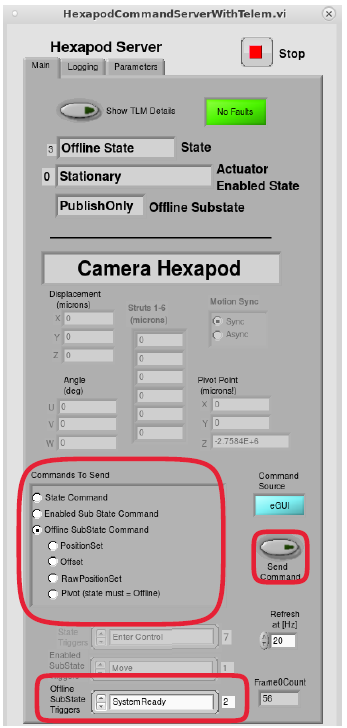
\includegraphics[width=1.79167in]{jira_imgs/1024.png}

}
\hdashrule[0.5ex]{\textwidth}{1pt}{3mm}
  Expected Result \\
{\footnotesize
The system transitions from the OfflineState/PublishOnly substate to the
OfflineState/AvailableState substate and the Command Source says
eGUI.\\[2\baselineskip]

}
\hdashrule[0.5ex]{\textwidth}{1pt}{3mm}
  Actual Result \\
{\footnotesize

}
\begin{tabular}{p{2cm}p{14cm}}
\toprule
Step 4 & Step Execution Status: \textbf{ Pass } \\ \hline
\end{tabular}
 Description \\
{\footnotesize
\textbf{OFFLINESTATE -\textgreater{} STANDBYSTATE}\\
Click on the State Command field in the Commands to Send section.\\
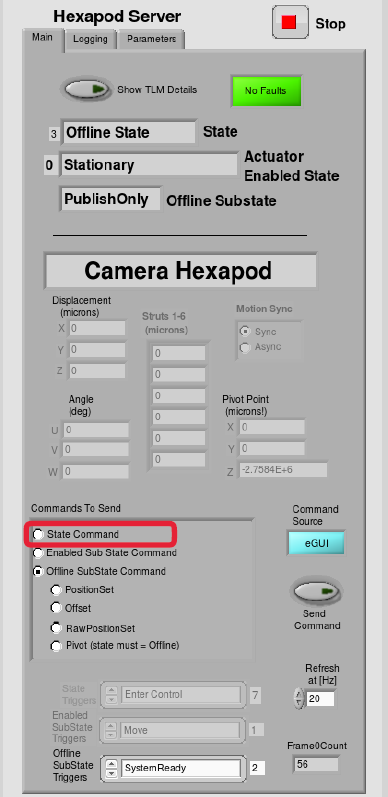
\includegraphics[width=1.79167in]{jira_imgs/1028.png}

}
\hdashrule[0.5ex]{\textwidth}{1pt}{3mm}
  Expected Result \\
{\footnotesize
The State Triggers dialogue box shown below becomes visible.\\
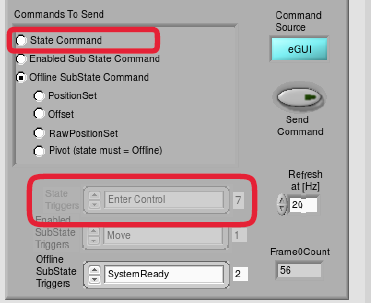
\includegraphics[width=1.79167in]{jira_imgs/1029.png}

}
\hdashrule[0.5ex]{\textwidth}{1pt}{3mm}
  Actual Result \\
{\footnotesize

}
\begin{tabular}{p{2cm}p{14cm}}
\toprule
Step 5 & Step Execution Status: \textbf{ Pass } \\ \hline
\end{tabular}
 Description \\
{\footnotesize
Scroll through the available trigger options to select ``Enter Control''
and click the Send Command button.

}
\hdashrule[0.5ex]{\textwidth}{1pt}{3mm}
  Expected Result \\
{\footnotesize
The system transitions to the Standby state and the primary state
display box at the top of the Main says Standby State.

}
\hdashrule[0.5ex]{\textwidth}{1pt}{3mm}
  Actual Result \\
{\footnotesize

}
\begin{tabular}{p{2cm}p{14cm}}
\toprule
Step 6 & Step Execution Status: \textbf{ Pass } \\ \hline
\end{tabular}
 Description \\
{\footnotesize
\textbf{STANDBYSTATE -\textgreater{} DISABLEDSTATE}\\
From the StandbyState, send a Start State command.

}
\hdashrule[0.5ex]{\textwidth}{1pt}{3mm}
  Expected Result \\
{\footnotesize
The system transitions into DisabledState and the current configuration
parameters are maintained from the default parameters or from the
previous DDS start command.~

}
\hdashrule[0.5ex]{\textwidth}{1pt}{3mm}
  Actual Result \\
{\footnotesize

}
\begin{tabular}{p{2cm}p{14cm}}
\toprule
Step 7 & Step Execution Status: \textbf{ Pass } \\ \hline
\end{tabular}
 Description \\
{\footnotesize
\textbf{DISABLEDSTATE -\textgreater{} ENABLEDSTATE}\\
From the DisabledState, send an Enable State Command.~

}
\hdashrule[0.5ex]{\textwidth}{1pt}{3mm}
  Expected Result \\
{\footnotesize
The system transitions into the EnabledState/Stationary substate, the
motor drives are enabled and and motion can be commanded.~

}
\hdashrule[0.5ex]{\textwidth}{1pt}{3mm}
  Actual Result \\
{\footnotesize

}
\begin{tabular}{p{2cm}p{14cm}}
\toprule
Step 8 & Step Execution Status: \textbf{ Pass } \\ \hline
\end{tabular}
 Description \\
{\footnotesize
\textless{}conditional state\textgreater{}\\
\textbf{FAULTSTATE}\\
If a Fault occurs in any of the other states, the system will
automatically transition to the Fault State. While in the Fault state,
send a clearError.\\
Note: If the fault that occurs goes through the interlock system, reset
the safety relay switch and send a clearError command.

}
\hdashrule[0.5ex]{\textwidth}{1pt}{3mm}
  Expected Result \\
{\footnotesize
The system transitions back to the OfflineState/PublishOnly substate.
(Go back to Step 3)

}
\hdashrule[0.5ex]{\textwidth}{1pt}{3mm}
  Actual Result \\
{\footnotesize

}
\begin{tabular}{p{2cm}p{14cm}}
\toprule
Step 9 & Step Execution Status: \textbf{ Fail } \\ \hline
\end{tabular}
 Description \\
{\footnotesize
\textbf{Follow \emph{3.3.1 Positioning} of the LSST Hexapods-Rotator
Acceptance Test Procedure, Sheet 23-24.}

}
\hdashrule[0.5ex]{\textwidth}{1pt}{3mm}
  Test Data \\
 {\footnotesize
\textbf{Deviation:~}Test this with no performance payload and at a
single elevation angle of zero degrees. Wait for 39s between movements.

}
\hdashrule[0.5ex]{\textwidth}{1pt}{3mm}
  Expected Result \\
{\footnotesize
The position of the hexapod is able to be commanded and no software
limits or limit switches are tripped.\\
The position of the hexapod is able to reach the commanded positions
within the absolute accuracy specifications of 25um in Z, 125um in XY,
205x10-5deg in RXRY, and 1500x10-5deg in RZ.

}
\hdashrule[0.5ex]{\textwidth}{1pt}{3mm}
  Actual Result \\
{\footnotesize
Failed: Camera hexapod actuator \#6 presented a dead zone at the second
move.

}
\hdashrule[0.5ex]{\textwidth}{1pt}{3mm}
  Issues found executing this step:  \\
{\footnotesize
\begin{itemize}
\item \href{https://jira.lsstcorp.org/browse/FRACAS-54}{FRACAS-54}~~Camera Hexapod actuator number 6 failure

\end{itemize}
}
\begin{tabular}{p{2cm}p{14cm}}
\toprule
Step 10 & Step Execution Status: \textbf{ Fail } \\ \hline
\end{tabular}
 Description \\
{\footnotesize
\textbf{Follow \emph{3.3.2 Centers of Rotation} of the LSST
Hexapods-Rotator Acceptance Test Procedure, Sheet 24-25.}

}
\hdashrule[0.5ex]{\textwidth}{1pt}{3mm}
  Test Data \\
 {\footnotesize
\textbf{Deviation:~}Record pivot position through the EUI. Wait for 39s
between movements.

}
\hdashrule[0.5ex]{\textwidth}{1pt}{3mm}
  Expected Result \\
{\footnotesize
The center of rotation is able to be moved.

}
\hdashrule[0.5ex]{\textwidth}{1pt}{3mm}
  Actual Result \\
{\footnotesize
The center of rotation and the z position in the EUI have an offset of
820.4mm

}
\hdashrule[0.5ex]{\textwidth}{1pt}{3mm}
  Issues found executing this step:  \\
{\footnotesize
\begin{itemize}
\item \href{https://jira.lsstcorp.org/browse/DM-29712}{DM-29712}~~The center of rotation and the z position in the EUI have an offset of
820.4mm

\end{itemize}
}
\begin{tabular}{p{2cm}p{14cm}}
\toprule
Step 11 & Step Execution Status: \textbf{ Pass } \\ \hline
\end{tabular}
 Description \\
{\footnotesize
\textbf{Follow \emph{3.3.3 Cross-Talk Motion~}of the LSST
Hexapods-Rotator Acceptance Test Procedure, Sheet 25.}

}
\hdashrule[0.5ex]{\textwidth}{1pt}{3mm}
  Expected Result \\
{\footnotesize
There is no cross-talk observed (actuator positioning errors and
erroneous geometry are minimal).

}
\hdashrule[0.5ex]{\textwidth}{1pt}{3mm}
  Actual Result \\
{\footnotesize
Observed positioning errors are within the acceptable error
range.\\[2\baselineskip]

}
\begin{tabular}{p{2cm}p{14cm}}
\toprule
Step 12 & Step Execution Status: \textbf{ Fail } \\ \hline
\end{tabular}
 Description \\
{\footnotesize
\textbf{Follow \emph{3.3.4 Radial (X and Y) Translational Range~}of the
LSST Hexapods-Rotator Acceptance Test Procedure, Sheet 25.}

}
\hdashrule[0.5ex]{\textwidth}{1pt}{3mm}
  Test Data \\
 {\footnotesize
\textbf{Deviation:~}Only test at a zero degree elevation angle. Wait for
39s between movements.

}
\hdashrule[0.5ex]{\textwidth}{1pt}{3mm}
  Expected Result \\
{\footnotesize
The hexapod is capable of moving to the positions in the XY plane listed
in the Acceptance Test Procedure.

}
\hdashrule[0.5ex]{\textwidth}{1pt}{3mm}
  Actual Result \\
{\footnotesize
Test failed, see detailed results from the laser tracking measurement
done by Roberto Tighe and Mario Rivera.\\
The error needs to be interpreted as: sqrt( (errX\^{}2) + (errY\^{}2) )
= 125um\\
Error is:\\
For test 3.3.5. (line 28) command position in XYZ is (7,6,0,0) and the
result is(7,52, -0.12, -0,02). That makes a difference of (80 um,
-120um, -20um).\\
The calculated result is: sqrt(120um\^{}2+ 80um\^{}2)= 148um?

}
\hdashrule[0.5ex]{\textwidth}{1pt}{3mm}
  Issues found executing this step:  \\
{\footnotesize
\begin{itemize}
\item \href{https://jira.lsstcorp.org/browse/LVV-19501}{LVV-19501}~~Camera Hexapod absolute XYZ value accuracy not reached

\end{itemize}
}
\begin{tabular}{p{2cm}p{14cm}}
\toprule
Step 13 & Step Execution Status: \textbf{ Fail } \\ \hline
\end{tabular}
 Description \\
{\footnotesize
\textbf{Follow \emph{3.3.6 Axial (Z) Translation Range~}of the LSST
Hexapods-Rotator Acceptance Test Procedure, Sheet 27.}

}
\hdashrule[0.5ex]{\textwidth}{1pt}{3mm}
  Test Data \\
 {\footnotesize
\textbf{Deviation:~}Only test at a zero degree elevation angle. Wait for
39s between movements.

}
\hdashrule[0.5ex]{\textwidth}{1pt}{3mm}
  Expected Result \\
{\footnotesize
The hexapod is capable of moving to the positions in the Z plane listed
in the Acceptance Test Procedure.~

}
\hdashrule[0.5ex]{\textwidth}{1pt}{3mm}
  Actual Result \\
{\footnotesize
Failed with error up to 60 micron.\\
For the absolute accuracy in Z of the four available values (lines
28,32,33 and 58, file attached to step 12) only the first value meets
the specification.\\
The error seems growing with more moves (20um,30um,40um,60um).

}
\hdashrule[0.5ex]{\textwidth}{1pt}{3mm}
  Issues found executing this step:  \\
{\footnotesize
\begin{itemize}
\item \href{https://jira.lsstcorp.org/browse/LVV-19501}{LVV-19501}~~Camera Hexapod absolute XYZ value accuracy not reached

\end{itemize}
}
\begin{tabular}{p{2cm}p{14cm}}
\toprule
Step 14 & Step Execution Status: \textbf{ Blocked } \\ \hline
\end{tabular}
 Description \\
{\footnotesize
\textbf{Follow \emph{3.3.8 Rotational Range Around X-Axis (Tip) and
Y-Axis (Tilt)~}of the LSST Hexapods-Rotator Acceptance Test Procedure,
Sheet 28-29.}

}
\hdashrule[0.5ex]{\textwidth}{1pt}{3mm}
  Test Data \\
 {\footnotesize
\textbf{Deviation:~}Only test at a zero degree elevation angle. Wait for
39s between movements.

}
\hdashrule[0.5ex]{\textwidth}{1pt}{3mm}
  Expected Result \\
{\footnotesize
The hexapod is capable of moving to the positions in the RXRY plane
listed in the Acceptance Test Procedure.

}
\hdashrule[0.5ex]{\textwidth}{1pt}{3mm}
  Actual Result \\
{\footnotesize
Blocked by \href{https://jira.lsstcorp.org/browse/FRACAS-54}{FRACAS-54}

}
\begin{tabular}{p{2cm}p{14cm}}
\toprule
Step 15 & Step Execution Status: \textbf{ Blocked } \\ \hline
\end{tabular}
 Description \\
{\footnotesize
\textbf{Follow \emph{3.3.10 Rotation Range Around Z-Axis (Twist)~}of the
LSST Hexapods-Rotator Acceptance Test Procedure, Sheet 30.}

}
\hdashrule[0.5ex]{\textwidth}{1pt}{3mm}
  Test Data \\
 {\footnotesize
\textbf{Deviation:~}Only test at a zero degree elevation angle. Wait for
39s between movements.

}
\hdashrule[0.5ex]{\textwidth}{1pt}{3mm}
  Expected Result \\
{\footnotesize
The hexapod is capable of moving to the positions in the RZ-axis listed
in the Acceptance Test Procedure.

}
\hdashrule[0.5ex]{\textwidth}{1pt}{3mm}
  Actual Result \\
{\footnotesize
Blocked by \href{https://jira.lsstcorp.org/browse/FRACAS-54}{FRACAS-54}

}
\begin{tabular}{p{2cm}p{14cm}}
\toprule
Step 16 & Step Execution Status: \textbf{ Not Executed } \\ \hline
\end{tabular}
 Description \\
{\footnotesize
\textbf{Follow \emph{3.3.12 Hexapod Repeatability} of the LSST
Hexapods-Rotato Acceptance Test Procedure, Sheet 31.}

}
\hdashrule[0.5ex]{\textwidth}{1pt}{3mm}
  Expected Result \\
{\footnotesize
The repeatability is as good as the test equipment can capture. This
means that the repeatability is limited by the resolution of the test
equipment.

}
\hdashrule[0.5ex]{\textwidth}{1pt}{3mm}
  Actual Result \\
{\footnotesize
Not executed. TBD after
\href{https://jira.lsstcorp.org/browse/FRACAS-54}{FRACAS-54} is solved.

}
\begin{tabular}{p{2cm}p{14cm}}
\toprule
Step 17 & Step Execution Status: \textbf{ Not Executed } \\ \hline
\end{tabular}
 Description \\
{\footnotesize
\textbf{Follow \emph{3.3.13 Hexapod Absolute Accuracy~}of the LSST
Hexapods-Rotator Acceptance Test Procedure, Sheet 38-42.}

}
\hdashrule[0.5ex]{\textwidth}{1pt}{3mm}
  Test Data \\
 {\footnotesize
\textbf{Deviation:~}Only test at a zero degree elevation angle. Wait for
39s between movements.

}
\hdashrule[0.5ex]{\textwidth}{1pt}{3mm}
  Expected Result \\
{\footnotesize
The accuracy of the hexapod is good enough to be consistently repeated.
The accuracy of the hexapod is at least the following: 25um in Z, 125um
in XY, 205x10-5deg in RXRY, and 1500x10-5deg in RZ.

}
\hdashrule[0.5ex]{\textwidth}{1pt}{3mm}
  Actual Result \\
{\footnotesize
Not executed. TBD after
\href{https://jira.lsstcorp.org/browse/FRACAS-54}{FRACAS-54} is solved.

}
\begin{tabular}{p{2cm}p{14cm}}
\toprule
Step 18 & Step Execution Status: \textbf{ Not Executed } \\ \hline
\end{tabular}
 Description \\
{\footnotesize
\textbf{Follow \emph{3.3.16 Hexapod Radial (X and Y) and Axial (Z)
Velocity Range} and~\emph{3.3.17 Hexapod Rotational Velocity~}of the
LSST Hexapods-Rotator Acceptance Test Procedure, Sheet 43-44.}

}
\hdashrule[0.5ex]{\textwidth}{1pt}{3mm}
  Test Data \\
 {\footnotesize
\textbf{Deviation:~}Only test this using synchronous mode. Wait for 39s
between movements.

}
\hdashrule[0.5ex]{\textwidth}{1pt}{3mm}
  Expected Result \\
{\footnotesize
The hexapod velocity exceeds the 152um/s in XY and 0.0039deg/s in RXYRY
and RZ requirements.

}
\hdashrule[0.5ex]{\textwidth}{1pt}{3mm}
  Actual Result \\
{\footnotesize
Not executed. TBD after
\href{https://jira.lsstcorp.org/browse/FRACAS-54}{FRACAS-54} is solved.

}
\begin{tabular}{p{2cm}p{14cm}}
\toprule
Step 19 & Step Execution Status: \textbf{ Not Executed } \\ \hline
\end{tabular}
 Description \\
{\footnotesize
\textbf{Follow \emph{3.3.18 Hexapod Heat Dissipation~}of the LSST
Hexapods-Rotator Acceptance Test Procedure, Sheet 44.}

}
\hdashrule[0.5ex]{\textwidth}{1pt}{3mm}
  Expected Result \\
{\footnotesize
The current measured by the inductive current probes is calculated to
meet the heat dissipation requirement.

}
\hdashrule[0.5ex]{\textwidth}{1pt}{3mm}
  Actual Result \\
{\footnotesize
Not executed. Temperature sensors are about to be installed. This will
be used to monitor the heat dissipation.

}

\paragraph{ LVV-T1599 - Camera Hexapod Software Functional Re-verification }\mbox{}\\

Version \textbf{1}.
Open  \href{https://jira.lsstcorp.org/secure/Tests.jspa#/testCase/LVV-T1599}{\textit{ LVV-T1599 } }
test case in Jira.

The objective of this test case is to re-verify the functional
requirements of the camera hexapod's software, after shipment of the
hardware from the vendor's facility to the Summit, as defined in \citeds{LTS-206}
and \citeds{LTS-160}. This test case will only exercise the functionality that
was executed previously and meets the following criteria:

\begin{itemize}
\tightlist
\item
  Only requires the camera hexapod to be operable
\item
  Only requires testing of the synchronous mode

  \begin{itemize}
  \tightlist
  \item
    \textbf{Asynchronous mode is not a standard mode of operation}
  \end{itemize}
\item
  Only requires the vendors EUI software and hardware via local control

  \begin{itemize}
  \tightlist
  \item
    Does \textbf{NOT} require integration with SAL
  \end{itemize}
\item
  Does \textbf{NOT} require the camera hexapod to be loaded with the
  camera simulated mass or actual camera hardware
\end{itemize}

The software functional requirements were previously verified during the
test campaign by the vendor at the vendor's facility and accepted by
LSST during the Factory Acceptance Test review. The test procedure used
during the vendor's acceptance testing is the \emph{LSST
Hexapods-Rotator Software Acceptance Test Procedure} which is attached
to this test case. The test steps of this test case are taken directly
from that document on how to perform the test in a similar way as was
performed previously and includes changes noted by the
vendor.\\[2\baselineskip]See the attached \emph{LSST Hexapod Operator's
Manual} for more information on how to operate the hexapod.

\textbf{ Preconditions}:\\
Prior to the execution of this test case to re-verify the Camera Hexapod
hardware functional requirements, the following Summit tasks must be
completed:

\begin{itemize}
\tightlist
\item
  The Hexapod has been installed on the camera cart

  \begin{itemize}
  \tightlist
  \item
    \url{https://jira.lsstcorp.org/browse/SUMMIT-3224}
  \end{itemize}
\item
  The Hexapod Controller has been deployed on the summit

  \begin{itemize}
  \tightlist
  \item
    \url{https://jira.lsstcorp.org/browse/SUMMIT-3229}
  \end{itemize}
\item
  Boxes for the Hexapod have been transported to the 3rd level

  \begin{itemize}
  \tightlist
  \item
    \url{https://jira.lsstcorp.org/browse/SUMMIT-3230}
  \end{itemize}
\item
  All Hexapod cables and cabinets have been prepared for integration
  with camera cart

  \begin{itemize}
  \tightlist
  \item
    \url{https://jira.lsstcorp.org/browse/SUMMIT-3231}
  \end{itemize}
\item
  The offset has been installed onto the integrating structure

  \begin{itemize}
  \tightlist
  \item
    \url{https://jira.lsstcorp.org/browse/SUMMIT-3293}
  \end{itemize}
\item
  The Camera Hexapod electrical connections have been tested

  \begin{itemize}
  \tightlist
  \item
    \url{https://jira.lsstcorp.org/browse/SUMMIT-3294}
  \end{itemize}
\end{itemize}

Execution status: {\bf Fail }

Final comment:\\

Issues found during the execution of LVV-T1599 test case:

\begin{itemize}
\item \href{https://jira.lsstcorp.org/browse/DM-29738}{DM-29738}~~Camera hexapod unexpectd behavior. ``positionSet'' command is accepted
in EnabledState.

\item \href{https://jira.lsstcorp.org/browse/DM-29788}{DM-29788}~~Camera Hexapod: The state of the state machine needs to be changed to
``clearError'' caused by unplugging the motor encoder.

\item \href{https://jira.lsstcorp.org/browse/DM-29791}{DM-29791}~~Camera Hexapod: The EUI needs to be restared to ``clearError'' caused by
unplugging the linear encoder.

\item \href{https://jira.lsstcorp.org/browse/DM-29792}{DM-29792}~~Camera Hexapod: The Enabled substate needs to be changed ``manually'' to
``clearError'' caused by unplugging the motor power cable.

\item \href{https://jira.lsstcorp.org/browse/DM-29793}{DM-29793}~~Camera Hexapod: The EUI needs to be restarted after re-plugging the
EtherCat cable

\end{itemize}

Detailed steps results:

\begin{tabular}{p{2cm}p{14cm}}
\toprule
Step 1 & Step Execution Status: \textbf{ Pass } \\ \hline
\end{tabular}
 Description \\
{\footnotesize
\textbf{STARTING THE EUI}\\[2\baselineskip]Double click the Hexapod GUI
Viewer desktop icon on the computer.

\begin{itemize}
\tightlist
\item
  This can be done on the Dell Management PC or another computer on the
  same network
\end{itemize}

}
\hdashrule[0.5ex]{\textwidth}{1pt}{3mm}
  Expected Result \\
{\footnotesize
A prompt to enter the password is shown.

}
\hdashrule[0.5ex]{\textwidth}{1pt}{3mm}
  Actual Result \\
{\footnotesize
The start-up procedure was working. For details see:
https://jira.lsstcorp.org/secure/Tests.jspa\#/testPlayer/testExecution/LVV-E1226

}
\begin{tabular}{p{2cm}p{14cm}}
\toprule
Step 2 & Step Execution Status: \textbf{ Pass } \\ \hline
\end{tabular}
 Description \\
{\footnotesize
Enter the password ``lsst-vnc''

\begin{itemize}
\tightlist
\item
  If the EUI isn't automatically up and running when the VNC opens,
  double click on the Hexapod-eGUI icon on the VNC viewer
\end{itemize}

}
\hdashrule[0.5ex]{\textwidth}{1pt}{3mm}
  Expected Result \\
{\footnotesize
The EUI is in the Offline State/PublishOnly substate and is able to
publish through SAL but cannot receive commands.

}
\hdashrule[0.5ex]{\textwidth}{1pt}{3mm}
  Actual Result \\
{\footnotesize

}
\begin{tabular}{p{2cm}p{14cm}}
\toprule
Step 3 & Step Execution Status: \textbf{ Pass } \\ \hline
\end{tabular}
 Description \\
{\footnotesize
\textbf{OFFLINESTATE/AVAILABLESTATE}\\
On the Main tab, select the ``Offline SubState Cmd'' field in the
Commands to Send section, set the Offline SubState Triggers to ``System
Ready'' and click on the Send Command button.\\
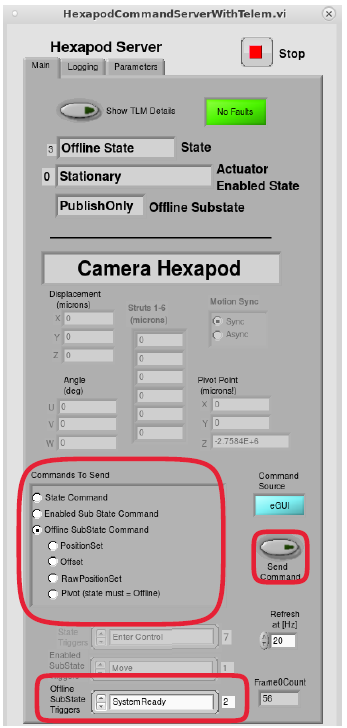
\includegraphics[width=1.79167in]{jira_imgs/1024.png}

}
\hdashrule[0.5ex]{\textwidth}{1pt}{3mm}
  Expected Result \\
{\footnotesize
The system transitions from the OfflineState/PublishOnly substate to the
OfflineState/AvailableState substate and the Command Source says
eGUI.\\[2\baselineskip]

}
\hdashrule[0.5ex]{\textwidth}{1pt}{3mm}
  Actual Result \\
{\footnotesize

}
\begin{tabular}{p{2cm}p{14cm}}
\toprule
Step 4 & Step Execution Status: \textbf{ Pass } \\ \hline
\end{tabular}
 Description \\
{\footnotesize
\textbf{OFFLINESTATE -\textgreater{} STANDBYSTATE}\\
Click on the State Command field in the Commands to Send section.\\
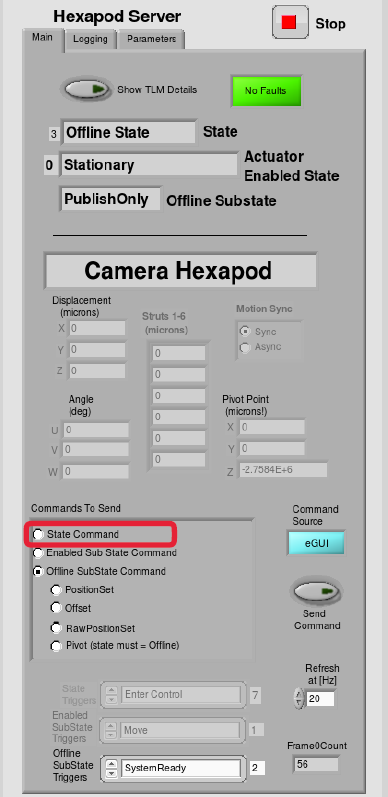
\includegraphics[width=1.79167in]{jira_imgs/1028.png}

}
\hdashrule[0.5ex]{\textwidth}{1pt}{3mm}
  Expected Result \\
{\footnotesize
The State Triggers dialogue box shown below becomes visible.\\
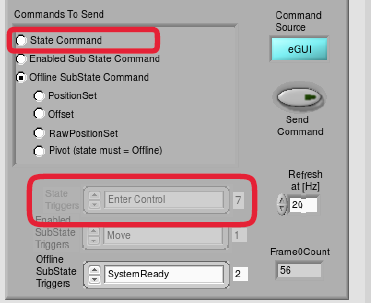
\includegraphics[width=1.79167in]{jira_imgs/1029.png}

}
\hdashrule[0.5ex]{\textwidth}{1pt}{3mm}
  Actual Result \\
{\footnotesize

}
\begin{tabular}{p{2cm}p{14cm}}
\toprule
Step 5 & Step Execution Status: \textbf{ Pass } \\ \hline
\end{tabular}
 Description \\
{\footnotesize
Scroll through the available trigger options to select ``Enter Control''
and click the Send Command button.

}
\hdashrule[0.5ex]{\textwidth}{1pt}{3mm}
  Expected Result \\
{\footnotesize
The system transitions to the Standby state and the primary state
display box at the top of the Main says Standby State.

}
\hdashrule[0.5ex]{\textwidth}{1pt}{3mm}
  Actual Result \\
{\footnotesize

}
\begin{tabular}{p{2cm}p{14cm}}
\toprule
Step 6 & Step Execution Status: \textbf{ Pass } \\ \hline
\end{tabular}
 Description \\
{\footnotesize
\textbf{STANDBYSTATE -\textgreater{} DISABLEDSTATE}\\
From the StandbyState, send a Start State command.

}
\hdashrule[0.5ex]{\textwidth}{1pt}{3mm}
  Expected Result \\
{\footnotesize
The system transitions into DisabledState and the current configuration
parameters are maintained from the default parameters or from the
previous DDS start command.~

}
\hdashrule[0.5ex]{\textwidth}{1pt}{3mm}
  Actual Result \\
{\footnotesize

}
\begin{tabular}{p{2cm}p{14cm}}
\toprule
Step 7 & Step Execution Status: \textbf{ Pass } \\ \hline
\end{tabular}
 Description \\
{\footnotesize
\textbf{DISABLEDSTATE -\textgreater{} ENABLEDSTATE}\\
From the DisabledState, send an Enable State Command.~

}
\hdashrule[0.5ex]{\textwidth}{1pt}{3mm}
  Expected Result \\
{\footnotesize
The system transitions into the EnabledState/Stationary substate, the
motor drives are enabled and and motion can be commanded.~

}
\hdashrule[0.5ex]{\textwidth}{1pt}{3mm}
  Actual Result \\
{\footnotesize

}
\begin{tabular}{p{2cm}p{14cm}}
\toprule
Step 8 & Step Execution Status: \textbf{ Pass } \\ \hline
\end{tabular}
 Description \\
{\footnotesize
\textless{}conditional state\textgreater{}\\
\textbf{FAULTSTATE}\\
If a Fault occurs in any of the other states, the system will
automatically transition to the Fault State. While in the Fault state,
send a clearError.\\
Note: If the fault that occurs goes through the interlock system, reset
the safety relay switch and send a clearError command.

}
\hdashrule[0.5ex]{\textwidth}{1pt}{3mm}
  Expected Result \\
{\footnotesize
The system transitions back to the OfflineState/PublishOnly substate.
(Go back to Step 3)

}
\hdashrule[0.5ex]{\textwidth}{1pt}{3mm}
  Actual Result \\
{\footnotesize

}
\begin{tabular}{p{2cm}p{14cm}}
\toprule
Step 9 & Step Execution Status: \textbf{ Pass } \\ \hline
\end{tabular}
 Description \\
{\footnotesize
\textbf{Section 3.1.1 of the attached Software Acceptance Test
Procedure\\
Test Sequence \#1 - Synchronous PositionSet and Move
Commands}\\[2\baselineskip]With the synchronous button enabled and in
enabled/stationary state, send a positionSet command of (0um, 0um,
200um, 0 deg, 0 deg, 0 deg) using the EUI.

}
\hdashrule[0.5ex]{\textwidth}{1pt}{3mm}
  Expected Result \\
{\footnotesize
The hexapod doesn't move.

}
\hdashrule[0.5ex]{\textwidth}{1pt}{3mm}
  Actual Result \\
{\footnotesize
Confirmed. The hexapod does not move.

}
\begin{tabular}{p{2cm}p{14cm}}
\toprule
Step 10 & Step Execution Status: \textbf{ Pass } \\ \hline
\end{tabular}
 Description \\
{\footnotesize
With the synchronous button enabled and in enabled/stationary state,
send a positionSet command of (2000um, -3500um, 200um, .01 deg, -.05deg,
.002deg) using the EUI.

}
\hdashrule[0.5ex]{\textwidth}{1pt}{3mm}
  Expected Result \\
{\footnotesize
The hexapod doesn't move.

}
\hdashrule[0.5ex]{\textwidth}{1pt}{3mm}
  Actual Result \\
{\footnotesize
Confirmed. The camera hexapod does not move.\\[2\baselineskip]

}
\begin{tabular}{p{2cm}p{14cm}}
\toprule
Step 11 & Step Execution Status: \textbf{ Fail } \\ \hline
\end{tabular}
 Description \\
{\footnotesize
Send a move command using the EUI.

}
\hdashrule[0.5ex]{\textwidth}{1pt}{3mm}
  Test Data \\
 {\footnotesize
Pivot position is shown in the GUI. Please mention in the results. Use
the MOOG pivot point for comparability with the previous results.

}
\hdashrule[0.5ex]{\textwidth}{1pt}{3mm}
  Expected Result \\
{\footnotesize
The hexapod moves to the last commanded position of (2000um, -3500um,
200um, .01 deg, -.05deg, .002deg) and the actuators complete the move at
nearly the same time as seen on the motion complete lights on the
telemetry screen.

}
\hdashrule[0.5ex]{\textwidth}{1pt}{3mm}
  Actual Result \\
{\footnotesize
The pivot position is ~-2.7584E+6.\\[2\baselineskip]On the first try the
hexapod went into fault state:\\
Apr 14 12:29:03 camhex journal: LSST Wrapper: SYNCHRONOUS CMD\\
Apr 14 12:29:03 camhex journal: LSST Wrapper: CMD: drive 0 pos -38451648
-38828365\\
Apr 14 12:29:03 camhex journal: LSST Wrapper: CMD: drive 0 accel 16191
12237\\
Apr 14 12:29:03 camhex journal: LSST Wrapper: CMD: drive 1 pos -42583267
-39107649\\
Apr 14 12:29:03 camhex journal: LSST Wrapper: CMD: drive 1 accel 49998
9408\\
Apr 14 12:29:03 camhex journal: LSST Wrapper: CMD: drive 2 pos -38510707
-41616191\\
Apr 14 12:29:03 camhex journal: LSST Wrapper: CMD: drive 2 accel 15428
16896\\
Apr 14 12:29:04 camhex journal: LSST Wrapper: Drive tracking error
reported\\
Apr 14 12:29:04 camhex journal: LSST Wrapper: Drive 1 latched fault
codes: 200 0\\
Apr 14 12:29:04 camhex journal: LSST Wrapper: Drive 1 status, codes:
7b98 5237\\
Apr 14 12:29:04 camhex journal: LSST Wrapper: Drive 1A state=Fault\\
Apr 14 12:29:04 camhex journal: LSST Wrapper: Drive 1B state=Operation
enabled\\
Apr 14 12:29:04 camhex journal: LSST Wrapper: Drive 1A lastFault=\\
Apr 14 12:29:04 camhex journal: LSST Wrapper: = generic fault\\
Apr 14 12:29:04 camhex journal: LSST Wrapper: Need to Halt: SETTING
quickstop=1\\
Apr 14 12:29:04 camhex journal: LSST Wrapper: Drive 0A state=Quick stop
active\\
Apr 14 12:29:04 camhex journal: LSST Wrapper: Drive 0B state=Quick stop
active\\
Apr 14 12:29:04 camhex journal: LSST Wrapper: Drive 1A state=Switch on
disabled\\
Apr 14 12:29:04 camhex journal: LSST Wrapper: Drive 1B state=Quick stop
active\\
Apr 14 12:29:04 camhex journal: LSST Wrapper: Drive 1A lastFault=\\
Apr 14 12:29:04 camhex journal: LSST Wrapper: = position tracking\\
Apr 14 12:29:04 camhex journal: LSST Wrapper: Drive 2A state=Quick stop
active\\
Apr 14 12:29:04 camhex journal: LSST Wrapper: Drive 2B state=Quick stop
active\\
Apr 14 12:29:04 camhex journal: LSST Wrapper: Drive 0A state=Switch on
disabled\\
Apr 14 12:29:04 camhex journal: LSST Wrapper: Drive 0B state=Switch on
disabled\\
Apr 14 12:29:04 camhex journal: LSST Wrapper: Drive 1A state=Switch on
disabled\\
Apr 14 12:29:04 camhex journal: LSST Wrapper: Drive 1B state=Switch on
disabled\\
Apr 14 12:29:04 camhex journal: LSST Wrapper: Drive 2A state=Switch on
disabled\\
Apr 14 12:29:04 camhex journal: LSST Wrapper: Drive 2B state=Switch on
disabled\\[2\baselineskip]Hexapod had moved a few microns in all axis\\
Hexapod in fault state\\
Actuator enabled State is Moving Pt-Pt\\
Stop command send.\\
Actuator enabled State is Moving Pt-Pt\\
Fault cleared through EUI.\\
State changed to Standby state\\
Actuator enabled State stays in Moving Pt-Pt\\
Fault cleared through EUI.\\
Actuator enabled State stays in Moving Pt-Pt\\
Start command send ---\textgreater{} state changed to disabled state\\
Actuator enabled State stays in Moving Pt-Pt\\
Enable command send ---\textgreater{} State changed to enabled state\\
Actuator enabled State stays in Moving Pt-Pt\\
Stop command send\\
Actuator enabled State changed to
Stationary\\[2\baselineskip]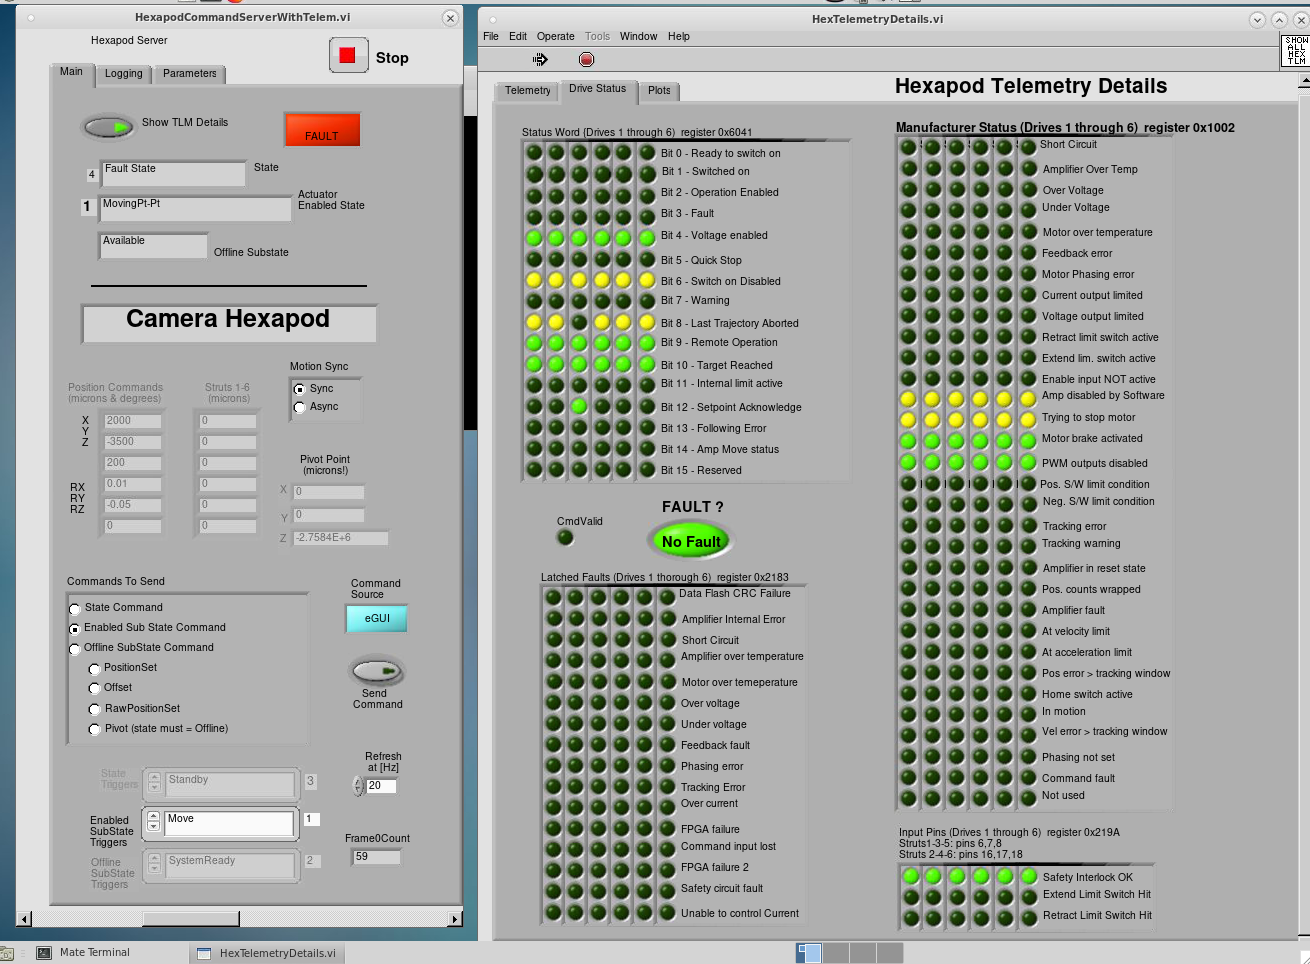
\includegraphics[width=3.12500in]{jira_imgs/1655.png}\\
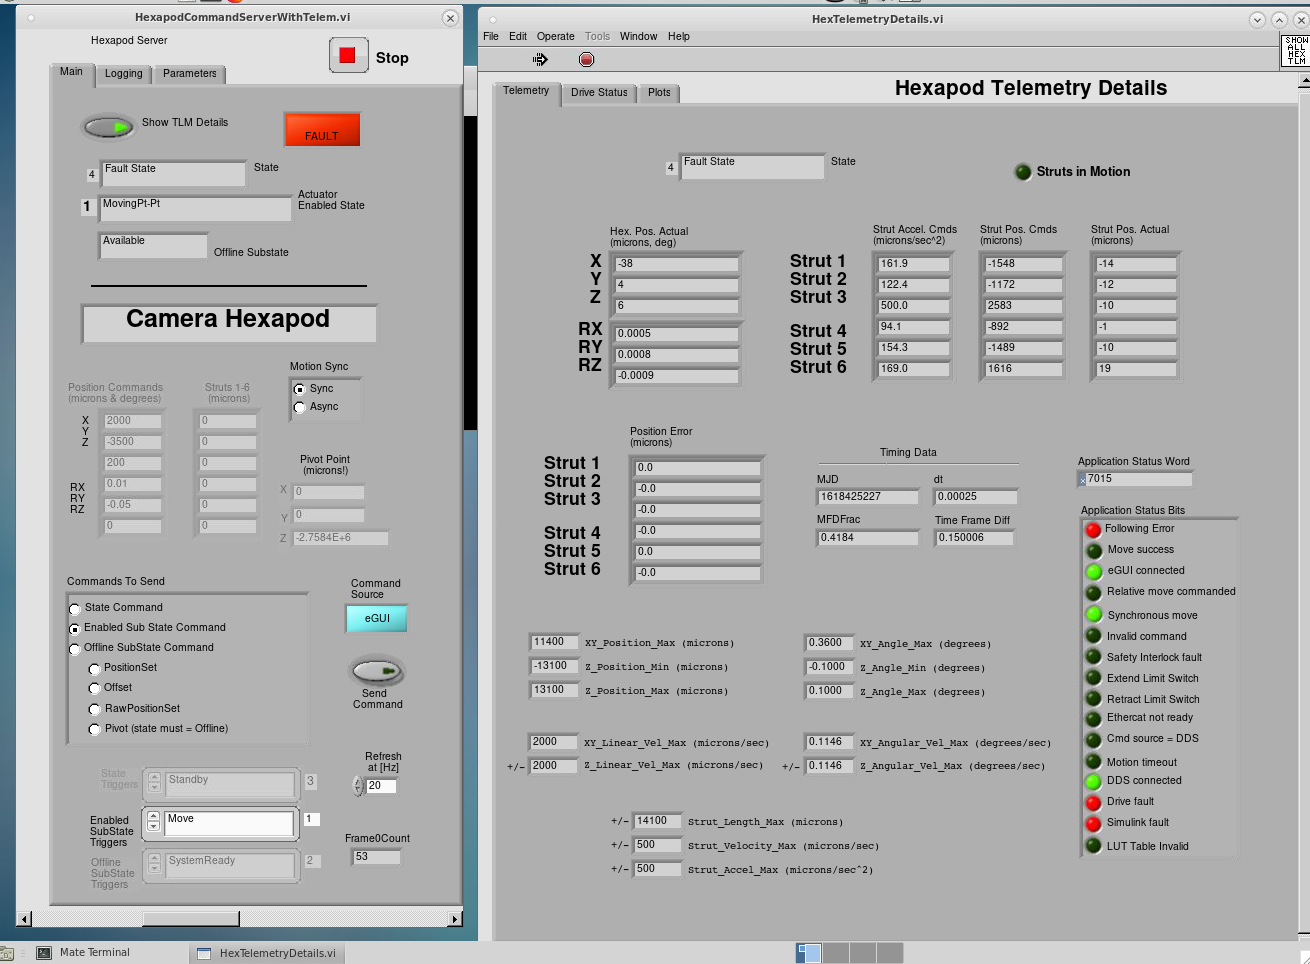
\includegraphics[width=3.12500in]{jira_imgs/1656.png}\\
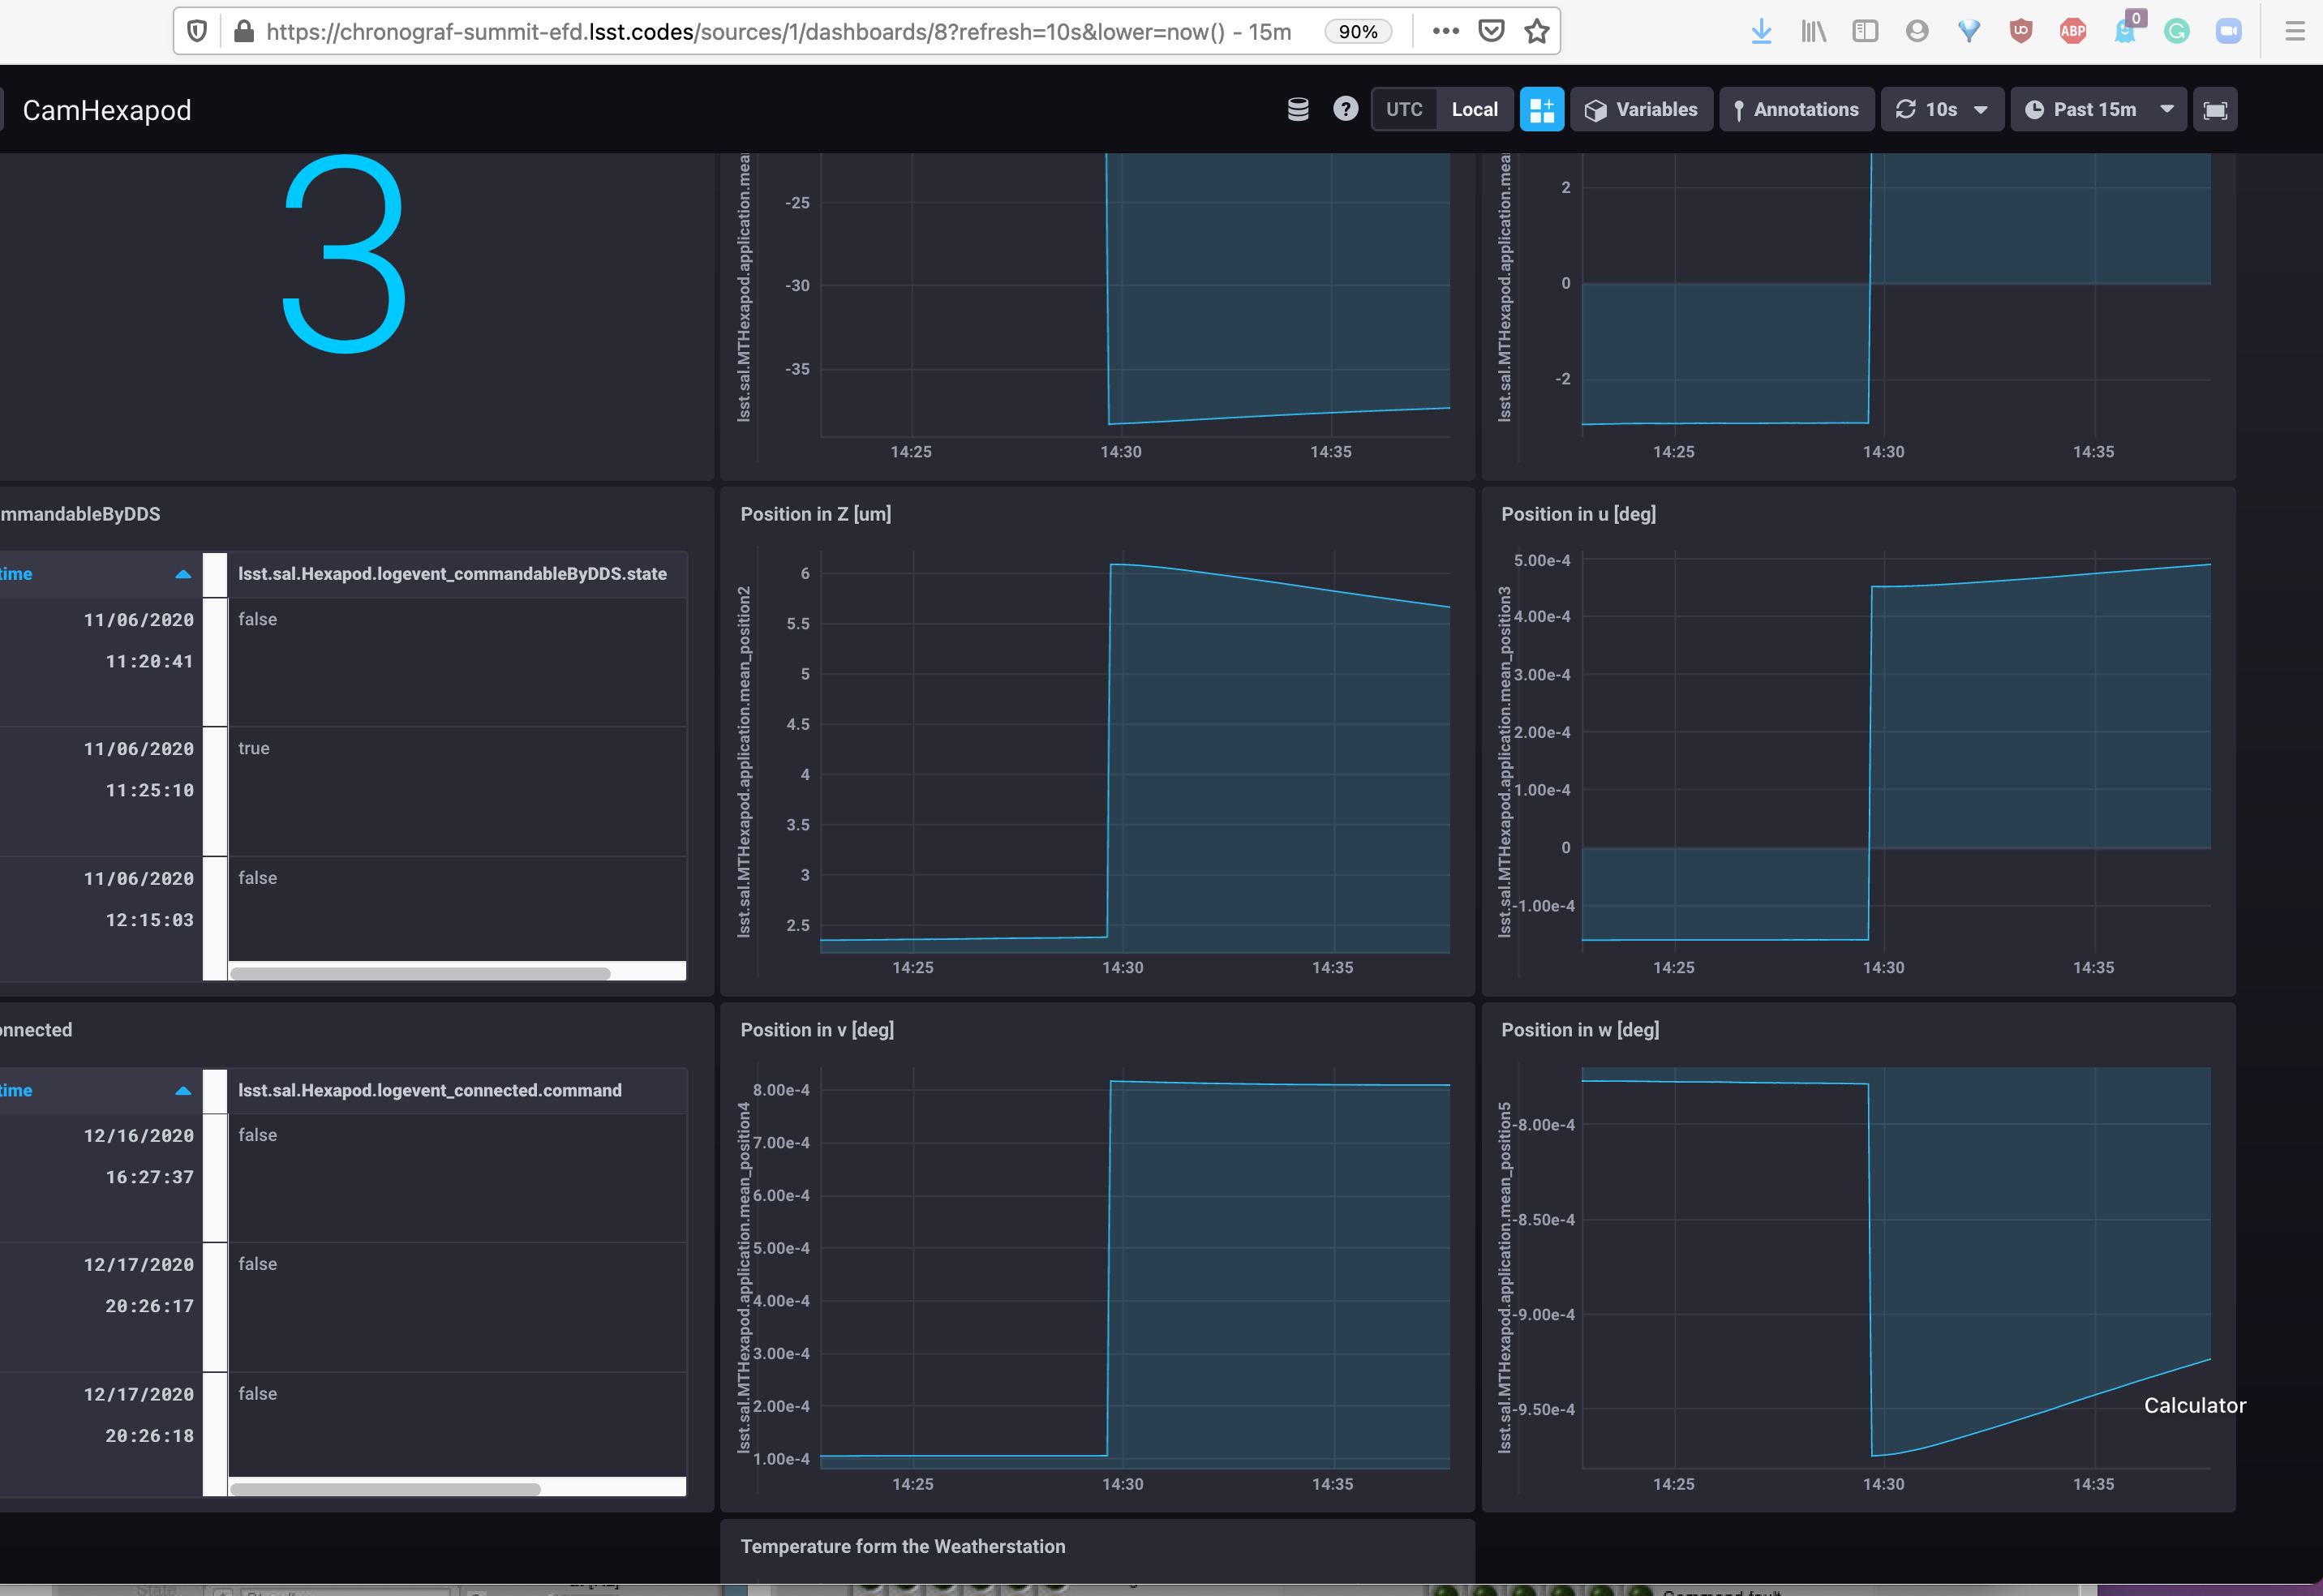
\includegraphics[width=3.12500in]{jira_imgs/1657.png}\\
Second try\\[2\baselineskip]Move command send nothing append\\
PositionSet command in Enabled state send\\
Move command send. Hexapod moved to the desired
position\\[2\baselineskip]This means the positionSet command is accepted
in EnabledState.\\
This is not expected from the EUI since positionSet is an
\textbf{Offline SubState} Command.

}
\hdashrule[0.5ex]{\textwidth}{1pt}{3mm}
  Issues found executing this step:  \\
{\footnotesize
\begin{itemize}
\item \href{https://jira.lsstcorp.org/browse/DM-29738}{DM-29738}~~Camera hexapod unexpectd behavior. ``positionSet'' command is accepted
in EnabledState.

\end{itemize}
}
\begin{tabular}{p{2cm}p{14cm}}
\toprule
Step 12 & Step Execution Status: \textbf{ Pass } \\ \hline
\end{tabular}
 Description \\
{\footnotesize
Wait 39s.

}
\hdashrule[0.5ex]{\textwidth}{1pt}{3mm}
  Expected Result \\
{\footnotesize

}
\hdashrule[0.5ex]{\textwidth}{1pt}{3mm}
  Actual Result \\
{\footnotesize

}
\begin{tabular}{p{2cm}p{14cm}}
\toprule
Step 13 & Step Execution Status: \textbf{ Pass } \\ \hline
\end{tabular}
 Description \\
{\footnotesize
\textbf{Section 3.1.1 of the attached Software Acceptance Test
Procedure\\
Test Sequence \#2 - Pivot, PositionSet and Move
Commands}\\[2\baselineskip]In enabled/stationary state and at the last
commanded position of (2000um, -3500um, 200um, .01 deg, -.05deg,
.002deg), change the pivot point from the default location to (0,0,0)
using the EUI.

}
\hdashrule[0.5ex]{\textwidth}{1pt}{3mm}
  Expected Result \\
{\footnotesize
The actuator positions do not change, but the hexapod position is
(-407um, -3982um, 199um, 0.01deg, -0.05deg, 0.002deg)

}
\hdashrule[0.5ex]{\textwidth}{1pt}{3mm}
  Actual Result \\
{\footnotesize
Confirmed. No movement. The position has changed to the expected value.

}
\begin{tabular}{p{2cm}p{14cm}}
\toprule
Step 14 & Step Execution Status: \textbf{ Pass } \\ \hline
\end{tabular}
 Description \\
{\footnotesize
In the enabled/stationary state, send a positionSet command of (2000um,
-3500um, 200um, .01 deg, -.05deg, .002deg) using the EUI.

}
\hdashrule[0.5ex]{\textwidth}{1pt}{3mm}
  Expected Result \\
{\footnotesize
The hexapod doesn't move.

}
\hdashrule[0.5ex]{\textwidth}{1pt}{3mm}
  Actual Result \\
{\footnotesize
State machine changed to enabled /stationary state. PositionSet command
send. No movement observed.

}
\begin{tabular}{p{2cm}p{14cm}}
\toprule
Step 15 & Step Execution Status: \textbf{ Pass } \\ \hline
\end{tabular}
 Description \\
{\footnotesize
Send a move command using the EUI.

}
\hdashrule[0.5ex]{\textwidth}{1pt}{3mm}
  Expected Result \\
{\footnotesize
The hexapod moves to the commanded position of (2000um, -3500um, 200um,
.01 deg, -.05deg, .002deg) and the actuators change position to account
for the new pivot point.

}
\hdashrule[0.5ex]{\textwidth}{1pt}{3mm}
  Actual Result \\
{\footnotesize
Confirmed the hexapod moved to the expected position.

}
\begin{tabular}{p{2cm}p{14cm}}
\toprule
Step 16 & Step Execution Status: \textbf{ Pass } \\ \hline
\end{tabular}
 Description \\
{\footnotesize
Wait 39s.

}
\hdashrule[0.5ex]{\textwidth}{1pt}{3mm}
  Expected Result \\
{\footnotesize

}
\hdashrule[0.5ex]{\textwidth}{1pt}{3mm}
  Actual Result \\
{\footnotesize

}
\begin{tabular}{p{2cm}p{14cm}}
\toprule
Step 17 & Step Execution Status: \textbf{ Pass } \\ \hline
\end{tabular}
 Description \\
{\footnotesize
\textbf{Section 3.1.1 of the attached Software Acceptance Test
Procedure\\
Test Sequence \#4 - Synchronous Offset and Move
Commands}\\[2\baselineskip]With the synchronous button enabled and in
enabled/stationary state, send a positionSet command of (500um, 800um,
200um, 0 deg, 0 deg, 0 deg).

}
\hdashrule[0.5ex]{\textwidth}{1pt}{3mm}
  Expected Result \\
{\footnotesize
The hexapod doesn't move.

}
\hdashrule[0.5ex]{\textwidth}{1pt}{3mm}
  Actual Result \\
{\footnotesize
Confirmed. positionSet command send. Hexapod did not move.

}
\begin{tabular}{p{2cm}p{14cm}}
\toprule
Step 18 & Step Execution Status: \textbf{ Pass w/ Deviation } \\ \hline
\end{tabular}
 Description \\
{\footnotesize
With the synchronous button enabled and in enabled/stationary state,
send an offset command of (0um, 0um, 2000um, 0 deg, 0 deg, 0 deg).~

}
\hdashrule[0.5ex]{\textwidth}{1pt}{3mm}
  Expected Result \\
{\footnotesize
The hexapod doesn't move.

}
\hdashrule[0.5ex]{\textwidth}{1pt}{3mm}
  Actual Result \\
{\footnotesize
Deviation: To avoid dead zone in actuator six command (0,0,-2000,0,0,0)
was send.\\
Hexapod did not move.

}
\begin{tabular}{p{2cm}p{14cm}}
\toprule
Step 19 & Step Execution Status: \textbf{ Pass w/ Deviation } \\ \hline
\end{tabular}
 Description \\
{\footnotesize
Send a move command.

}
\hdashrule[0.5ex]{\textwidth}{1pt}{3mm}
  Expected Result \\
{\footnotesize
The hexapod moves only 2000um in Z from the previous position. Since the
test is done in synchronous mode the actuators are expected to complete
the move at nearly the same time as seen on the motion complete lights
on the telemetry screen.

}
\hdashrule[0.5ex]{\textwidth}{1pt}{3mm}
  Actual Result \\
{\footnotesize
Deviation: To avoid dead zone in actuator six command (0,0,-2000,0,0,0)
was send.\\
Hexapod moved to (200,-3500-1800,0.01,-0.05)\\
The actuators finished the move nearly at the same time.

}
\begin{tabular}{p{2cm}p{14cm}}
\toprule
Step 20 & Step Execution Status: \textbf{ Pass } \\ \hline
\end{tabular}
 Description \\
{\footnotesize
Wait 39s.

}
\hdashrule[0.5ex]{\textwidth}{1pt}{3mm}
  Expected Result \\
{\footnotesize

}
\hdashrule[0.5ex]{\textwidth}{1pt}{3mm}
  Actual Result \\
{\footnotesize

}
\begin{tabular}{p{2cm}p{14cm}}
\toprule
Step 21 & Step Execution Status: \textbf{ Pass } \\ \hline
\end{tabular}
 Description \\
{\footnotesize
\textbf{Instead of Asynchronous Test}\\
{With the synchronous button enabled and in enabled/stationary
state,}{\textbf{~}}{s}end a position set command of (0um, 0um, 0um,
0.1deg, 0deg, 0deg)

}
\hdashrule[0.5ex]{\textwidth}{1pt}{3mm}
  Expected Result \\
{\footnotesize
The hexapod doesn't move.

}
\hdashrule[0.5ex]{\textwidth}{1pt}{3mm}
  Actual Result \\
{\footnotesize
\begin{enumerate}
\tightlist
\item
  Hexapod moved back to (0,0,0,0,0,0)
\item
  positionSet command send.
\item
  No movement.
\end{enumerate}

}
\begin{tabular}{p{2cm}p{14cm}}
\toprule
Step 22 & Step Execution Status: \textbf{ Pass } \\ \hline
\end{tabular}
 Description \\
{\footnotesize
Send a move command.

}
\hdashrule[0.5ex]{\textwidth}{1pt}{3mm}
  Expected Result \\
{\footnotesize
The hexapod moves to the commanded position of (0um, 0um, 0um, 0.1deg,
0deg, 0deg)

}
\hdashrule[0.5ex]{\textwidth}{1pt}{3mm}
  Actual Result \\
{\footnotesize
Hexapod moves to the expected position as commanded.

}
\begin{tabular}{p{2cm}p{14cm}}
\toprule
Step 23 & Step Execution Status: \textbf{ Pass } \\ \hline
\end{tabular}
 Description \\
{\footnotesize
Wait 39s.

}
\hdashrule[0.5ex]{\textwidth}{1pt}{3mm}
  Expected Result \\
{\footnotesize

}
\hdashrule[0.5ex]{\textwidth}{1pt}{3mm}
  Actual Result \\
{\footnotesize

}
\begin{tabular}{p{2cm}p{14cm}}
\toprule
Step 24 & Step Execution Status: \textbf{ Pass } \\ \hline
\end{tabular}
 Description \\
{\footnotesize
With the synchronous button enabled and in enabled/stationary
state,\textbf{~}send a position set command of (0um, 0um, 0um, 0deg,
0.1deg, 0deg)

}
\hdashrule[0.5ex]{\textwidth}{1pt}{3mm}
  Expected Result \\
{\footnotesize
The hexapod doesn't move.

}
\hdashrule[0.5ex]{\textwidth}{1pt}{3mm}
  Actual Result \\
{\footnotesize
\begin{enumerate}
\tightlist
\item
  Hexapod moved back to (0,0,0,0,0,0)
\item
  positionSet command send.
\item
  No movement.
\end{enumerate}

}
\begin{tabular}{p{2cm}p{14cm}}
\toprule
Step 25 & Step Execution Status: \textbf{ Pass } \\ \hline
\end{tabular}
 Description \\
{\footnotesize
Send a move command.

}
\hdashrule[0.5ex]{\textwidth}{1pt}{3mm}
  Expected Result \\
{\footnotesize
The hexapod moves to the commanded position of (0um, 0um, 0um, 0deg,
0.1deg, 0deg)

}
\hdashrule[0.5ex]{\textwidth}{1pt}{3mm}
  Actual Result \\
{\footnotesize
Hexapod moves to the expected position as commanded.

}
\begin{tabular}{p{2cm}p{14cm}}
\toprule
Step 26 & Step Execution Status: \textbf{ Pass } \\ \hline
\end{tabular}
 Description \\
{\footnotesize
Wait 39s.

}
\hdashrule[0.5ex]{\textwidth}{1pt}{3mm}
  Expected Result \\
{\footnotesize

}
\hdashrule[0.5ex]{\textwidth}{1pt}{3mm}
  Actual Result \\
{\footnotesize

}
\begin{tabular}{p{2cm}p{14cm}}
\toprule
Step 27 & Step Execution Status: \textbf{ Pass } \\ \hline
\end{tabular}
 Description \\
{\footnotesize
With the synchronous button enabled and in enabled/stationary
state,\textbf{~}send a position set command of (0um, 0um, 0um, 0.1deg,
0.1deg, 0deg)

}
\hdashrule[0.5ex]{\textwidth}{1pt}{3mm}
  Expected Result \\
{\footnotesize
The hexapod doesn't move.

}
\hdashrule[0.5ex]{\textwidth}{1pt}{3mm}
  Actual Result \\
{\footnotesize
\begin{enumerate}
\tightlist
\item
  positionSet command send.
\item
  No movement.
\end{enumerate}

}
\begin{tabular}{p{2cm}p{14cm}}
\toprule
Step 28 & Step Execution Status: \textbf{ Pass } \\ \hline
\end{tabular}
 Description \\
{\footnotesize
Send a move command.

}
\hdashrule[0.5ex]{\textwidth}{1pt}{3mm}
  Expected Result \\
{\footnotesize
The hexapod moves to the commanded position of (0um, 0um, 0um, 0.1deg,
0.1deg, 0deg)

}
\hdashrule[0.5ex]{\textwidth}{1pt}{3mm}
  Actual Result \\
{\footnotesize
Hexapod moves to the expected position as commanded.

}
\begin{tabular}{p{2cm}p{14cm}}
\toprule
Step 29 & Step Execution Status: \textbf{ Pass } \\ \hline
\end{tabular}
 Description \\
{\footnotesize
Wait 39s.

}
\hdashrule[0.5ex]{\textwidth}{1pt}{3mm}
  Expected Result \\
{\footnotesize

}
\hdashrule[0.5ex]{\textwidth}{1pt}{3mm}
  Actual Result \\
{\footnotesize

}
\begin{tabular}{p{2cm}p{14cm}}
\toprule
Step 30 & Step Execution Status: \textbf{ Pass } \\ \hline
\end{tabular}
 Description \\
{\footnotesize
\textbf{Section 3.1.1 of the attached Software Acceptance Test
Procedure\\
Test Sequence \#5 - Stop Commands}\\[2\baselineskip]In
enabled/stationary state, send a position set command of (0um, 0um,
5000um, 0 deg, 0 deg, 0 deg).

}
\hdashrule[0.5ex]{\textwidth}{1pt}{3mm}
  Expected Result \\
{\footnotesize
The hexapod doesn't move.

}
\hdashrule[0.5ex]{\textwidth}{1pt}{3mm}
  Actual Result \\
{\footnotesize
Deviation: To avoid dead zone in actuator six command (0,0,-5000,0,0,0)
was send.\\
Hexapod did not move.

}
\begin{tabular}{p{2cm}p{14cm}}
\toprule
Step 31 & Step Execution Status: \textbf{ Pass } \\ \hline
\end{tabular}
 Description \\
{\footnotesize
Send a move command.

}
\hdashrule[0.5ex]{\textwidth}{1pt}{3mm}
  Expected Result \\
{\footnotesize
The hexapod starts to move to the commanded position.

}
\hdashrule[0.5ex]{\textwidth}{1pt}{3mm}
  Actual Result \\
{\footnotesize
Confirmed hexapod starts movement.\\[2\baselineskip]

}
\begin{tabular}{p{2cm}p{14cm}}
\toprule
Step 32 & Step Execution Status: \textbf{ Pass } \\ \hline
\end{tabular}
 Description \\
{\footnotesize
Wait 3s.

}
\hdashrule[0.5ex]{\textwidth}{1pt}{3mm}
  Expected Result \\
{\footnotesize

}
\hdashrule[0.5ex]{\textwidth}{1pt}{3mm}
  Actual Result \\
{\footnotesize

}
\begin{tabular}{p{2cm}p{14cm}}
\toprule
Step 33 & Step Execution Status: \textbf{ Pass } \\ \hline
\end{tabular}
 Description \\
{\footnotesize
Send the stop command.~

}
\hdashrule[0.5ex]{\textwidth}{1pt}{3mm}
  Expected Result \\
{\footnotesize
The hexapod quickly comes to a stop prior to reaching the commanded
position.

}
\hdashrule[0.5ex]{\textwidth}{1pt}{3mm}
  Actual Result \\
{\footnotesize
Confirmed hexapod stopped nearly immediately.

}
\begin{tabular}{p{2cm}p{14cm}}
\toprule
Step 34 & Step Execution Status: \textbf{ Pass } \\ \hline
\end{tabular}
 Description \\
{\footnotesize
\textbf{Section 3.3.1 EUI Tests of the attached Software Acceptance Test
Procedure}\\
At startup, confirm that the system starts in the Offline/PublishOnly
state.

}
\hdashrule[0.5ex]{\textwidth}{1pt}{3mm}
  Expected Result \\
{\footnotesize
The rotator starts in the Offline/PublishOnly state.

}
\hdashrule[0.5ex]{\textwidth}{1pt}{3mm}
  Actual Result \\
{\footnotesize
Confirmed, the hexapod starts in Offline/PublishOnly state.

}
\begin{tabular}{p{2cm}p{14cm}}
\toprule
Step 35 & Step Execution Status: \textbf{ Pass } \\ \hline
\end{tabular}
 Description \\
{\footnotesize
Send an offline substate trigger of systemReady.

}
\hdashrule[0.5ex]{\textwidth}{1pt}{3mm}
  Expected Result \\
{\footnotesize
The system transitions into the Offline/Available substate.

}
\hdashrule[0.5ex]{\textwidth}{1pt}{3mm}
  Actual Result \\
{\footnotesize
Confirmed, The system transitions into the Offline/Available substrate
upon receiving the SystemReady offline substate trigger.

}
\begin{tabular}{p{2cm}p{14cm}}
\toprule
Step 36 & Step Execution Status: \textbf{ Pass } \\ \hline
\end{tabular}
 Description \\
{\footnotesize
Send an EnterControl trigger.

}
\hdashrule[0.5ex]{\textwidth}{1pt}{3mm}
  Expected Result \\
{\footnotesize
The system transitions from Offline/Available to Standby state.

}
\hdashrule[0.5ex]{\textwidth}{1pt}{3mm}
  Actual Result \\
{\footnotesize
Confirmed

}
\begin{tabular}{p{2cm}p{14cm}}
\toprule
Step 37 & Step Execution Status: \textbf{ Pass } \\ \hline
\end{tabular}
 Description \\
{\footnotesize
Send a Start trigger.

}
\hdashrule[0.5ex]{\textwidth}{1pt}{3mm}
  Expected Result \\
{\footnotesize
The system transitions from Standby to Disabled state.

}
\hdashrule[0.5ex]{\textwidth}{1pt}{3mm}
  Actual Result \\
{\footnotesize
Confirmed

}
\begin{tabular}{p{2cm}p{14cm}}
\toprule
Step 38 & Step Execution Status: \textbf{ Pass } \\ \hline
\end{tabular}
 Description \\
{\footnotesize
Send an Enable trigger.

}
\hdashrule[0.5ex]{\textwidth}{1pt}{3mm}
  Expected Result \\
{\footnotesize
The system transitions from Disabled to Enabled state.

}
\hdashrule[0.5ex]{\textwidth}{1pt}{3mm}
  Actual Result \\
{\footnotesize
Confirmed

}
\begin{tabular}{p{2cm}p{14cm}}
\toprule
Step 39 & Step Execution Status: \textbf{ Pass } \\ \hline
\end{tabular}
 Description \\
{\footnotesize
Send a Disable trigger.

}
\hdashrule[0.5ex]{\textwidth}{1pt}{3mm}
  Expected Result \\
{\footnotesize
The system transitions from Enabled to Disabled state.

}
\hdashrule[0.5ex]{\textwidth}{1pt}{3mm}
  Actual Result \\
{\footnotesize
Confirmed

}
\begin{tabular}{p{2cm}p{14cm}}
\toprule
Step 40 & Step Execution Status: \textbf{ Pass } \\ \hline
\end{tabular}
 Description \\
{\footnotesize
Send a Standby trigger.

}
\hdashrule[0.5ex]{\textwidth}{1pt}{3mm}
  Expected Result \\
{\footnotesize
The system transitions from Disabled state to Standby state.

}
\hdashrule[0.5ex]{\textwidth}{1pt}{3mm}
  Actual Result \\
{\footnotesize
Confirmed

}
\begin{tabular}{p{2cm}p{14cm}}
\toprule
Step 41 & Step Execution Status: \textbf{ Pass } \\ \hline
\end{tabular}
 Description \\
{\footnotesize
Send a exitControl trigger.

}
\hdashrule[0.5ex]{\textwidth}{1pt}{3mm}
  Expected Result \\
{\footnotesize
The system transitions from Standby state to Offline state.

}
\hdashrule[0.5ex]{\textwidth}{1pt}{3mm}
  Actual Result \\
{\footnotesize
Confirmed. Transitions to OfflineState/Available.

}
\begin{tabular}{p{2cm}p{14cm}}
\toprule
Step 42 & Step Execution Status: \textbf{ Pass } \\ \hline
\end{tabular}
 Description \\
{\footnotesize
Return to the Enabled state and trip the safety interlock switch.

}
\hdashrule[0.5ex]{\textwidth}{1pt}{3mm}
  Expected Result \\
{\footnotesize
The system transitions to Fault state.

}
\hdashrule[0.5ex]{\textwidth}{1pt}{3mm}
  Actual Result \\
{\footnotesize
Felipe tried the limit switches. Behavior was as expected.

}
\begin{tabular}{p{2cm}p{14cm}}
\toprule
Step 43 & Step Execution Status: \textbf{ Pass } \\ \hline
\end{tabular}
 Description \\
{\footnotesize
Reset the safety interlock and send a ClearError trigger.

}
\hdashrule[0.5ex]{\textwidth}{1pt}{3mm}
  Expected Result \\
{\footnotesize
The EUI, upon receiving the ¨clearError¨ trigger, transitions from
FaultState to OfflineState/PublishOnly when the system was in any of the
OfflineStates before the error occurred. The EUI, upon receiving the
``clearError'' trigger, transitions to StandbyState when it was in
EnableState or DisableState before the error occurred.

}
\hdashrule[0.5ex]{\textwidth}{1pt}{3mm}
  Actual Result \\
{\footnotesize
Sending a clearError command transitions the state machine into
StandbyState.

}
\begin{tabular}{p{2cm}p{14cm}}
\toprule
Step 44 & Step Execution Status: \textbf{ Pass } \\ \hline
\end{tabular}
 Description \\
{\footnotesize
\textbf{Section 4.1 Hexapod Events of the attached Software Acceptance
Test Procedure}\\[2\baselineskip]In the Enabled/Stationary state, unplug
a motor encoder cable for one of the actuators.

}
\hdashrule[0.5ex]{\textwidth}{1pt}{3mm}
  Test Data \\
 {\footnotesize
\textbf{Deviation:~}Perform the following set of steps using the EUI
instead of the DDS and verify the events are displayed on the EUI.

}
\hdashrule[0.5ex]{\textwidth}{1pt}{3mm}
  Expected Result \\
{\footnotesize
A Drive Fault error event is created and the system transitions to Fault
state.

}
\hdashrule[0.5ex]{\textwidth}{1pt}{3mm}
  Actual Result \\
{\footnotesize
Strut 11 motor cable disconnection detected.\\
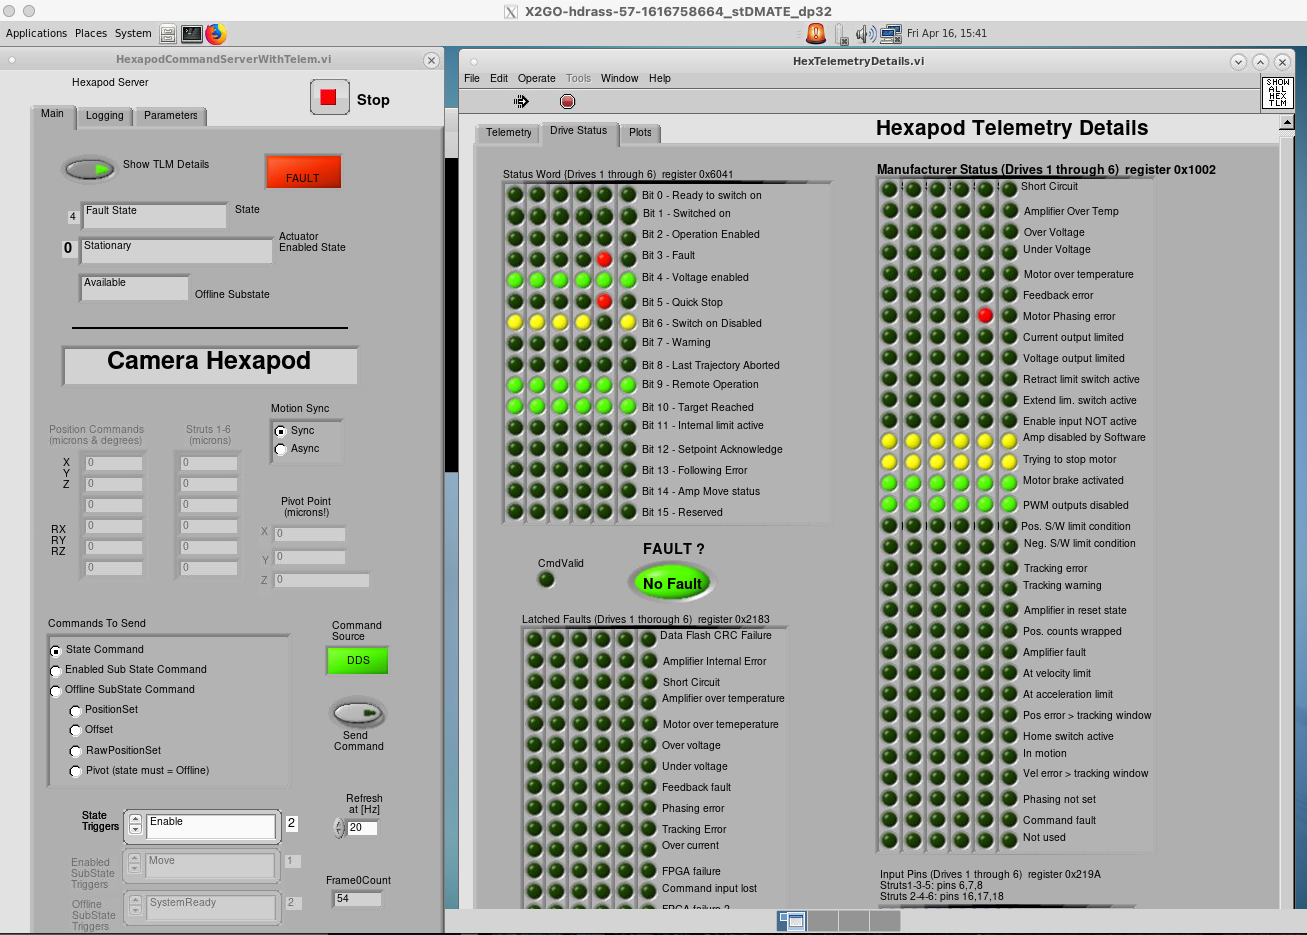
\includegraphics[width=3.12500in]{jira_imgs/1668.png}\\
no message at lsst.sal.Script.logevent\_logMessage.message

}
\begin{tabular}{p{2cm}p{14cm}}
\toprule
Step 45 & Step Execution Status: \textbf{ Fail } \\ \hline
\end{tabular}
 Description \\
{\footnotesize
Send the ``clearError'' trigger and bring the system to the
Enabled/Stationary state.

}
\hdashrule[0.5ex]{\textwidth}{1pt}{3mm}
  Expected Result \\
{\footnotesize
The system is in the Enabled/Stationary state and ready to be commanded.

}
\hdashrule[0.5ex]{\textwidth}{1pt}{3mm}
  Actual Result \\
{\footnotesize
``clearError'' cleared Drive fault but not Simulink.\\
Status changed to disabled.\\
``clearError'' cleared Simulink.

}
\hdashrule[0.5ex]{\textwidth}{1pt}{3mm}
  Issues found executing this step:  \\
{\footnotesize
\begin{itemize}
\item \href{https://jira.lsstcorp.org/browse/DM-29788}{DM-29788}~~Camera Hexapod: The state of the state machine needs to be changed to
``clearError'' caused by unplugging the motor encoder.

\end{itemize}
}
\begin{tabular}{p{2cm}p{14cm}}
\toprule
Step 46 & Step Execution Status: \textbf{ Pass } \\ \hline
\end{tabular}
 Description \\
{\footnotesize
In the Enabled/Stationary state, unplug a linear encoder cable for one
of the actuators.~

}
\hdashrule[0.5ex]{\textwidth}{1pt}{3mm}
  Expected Result \\
{\footnotesize
A Drive Fault error event is created and the system transitions to Fault
state.

}
\hdashrule[0.5ex]{\textwidth}{1pt}{3mm}
  Actual Result \\
{\footnotesize
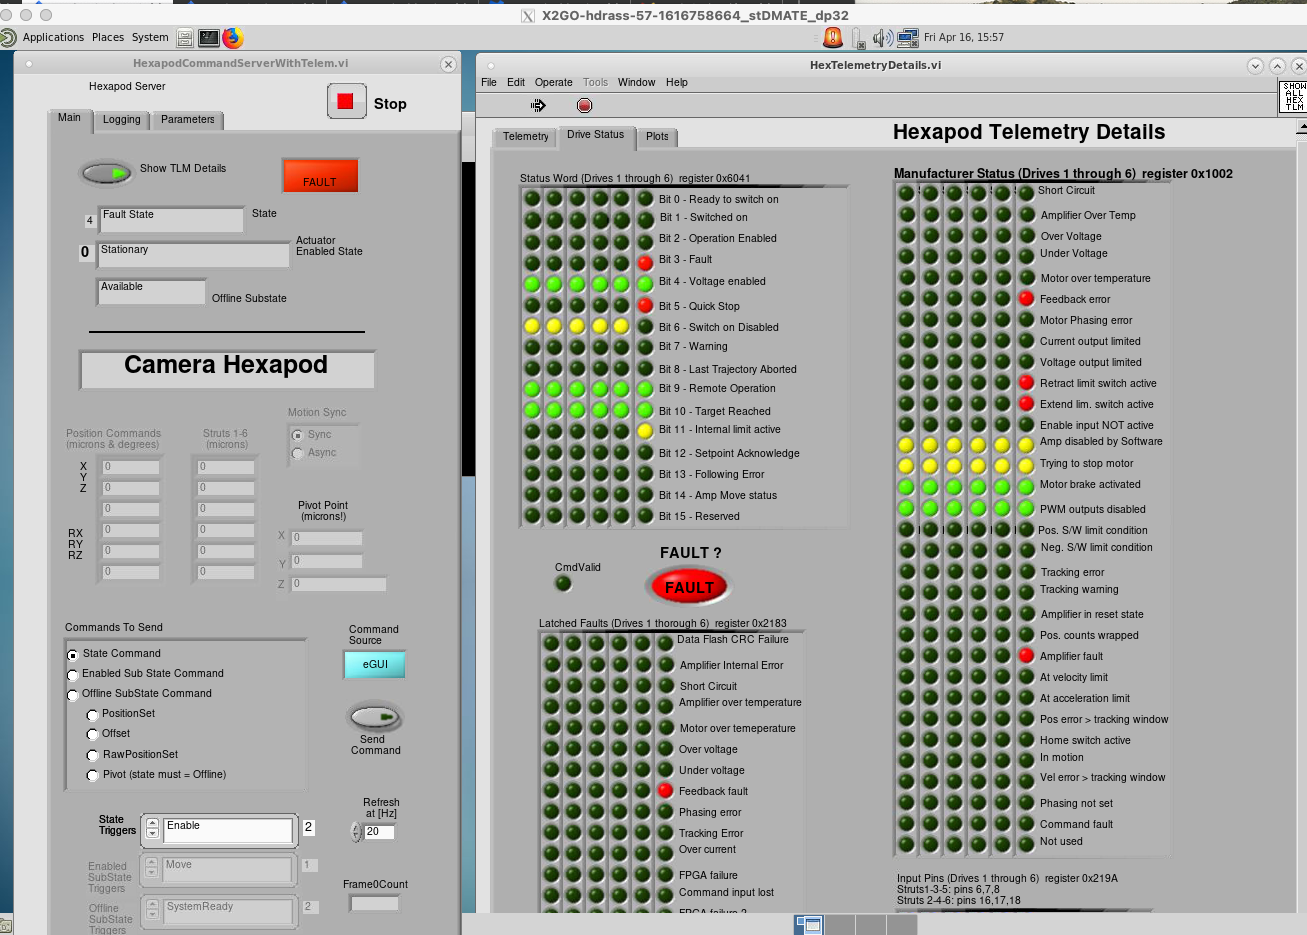
\includegraphics[width=3.12500in]{jira_imgs/1669.png}\\
Confirmed! For strut 12.

}
\begin{tabular}{p{2cm}p{14cm}}
\toprule
Step 47 & Step Execution Status: \textbf{ Fail } \\ \hline
\end{tabular}
 Description \\
{\footnotesize
Send the ``clearError'' trigger and bring the system to the
Enabled/Stationary state.

}
\hdashrule[0.5ex]{\textwidth}{1pt}{3mm}
  Expected Result \\
{\footnotesize
The system is in the Enabled/Stationary state and ready to be commanded.

}
\hdashrule[0.5ex]{\textwidth}{1pt}{3mm}
  Actual Result \\
{\footnotesize
Fault can not be cleared from the EUI.\\
Rest bottom did not reset the fault.\\
Restarting the EUI rested the fault.

}
\hdashrule[0.5ex]{\textwidth}{1pt}{3mm}
  Issues found executing this step:  \\
{\footnotesize
\begin{itemize}
\item \href{https://jira.lsstcorp.org/browse/DM-29791}{DM-29791}~~Camera Hexapod: The EUI needs to be restared to ``clearError'' caused by
unplugging the linear encoder.

\end{itemize}
}
\begin{tabular}{p{2cm}p{14cm}}
\toprule
Step 48 & Step Execution Status: \textbf{ Pass } \\ \hline
\end{tabular}
 Description \\
{\footnotesize
In the Enabled/Stationary state, unplug a linear encoder cable for one
of the actuators.~

}
\hdashrule[0.5ex]{\textwidth}{1pt}{3mm}
  Expected Result \\
{\footnotesize
A Drive Fault error event is created and the system transitions to Fault
state.

}
\hdashrule[0.5ex]{\textwidth}{1pt}{3mm}
  Actual Result \\
{\footnotesize
Duplicate of step 46.

}
\begin{tabular}{p{2cm}p{14cm}}
\toprule
Step 49 & Step Execution Status: \textbf{ Not Executed } \\ \hline
\end{tabular}
 Description \\
{\footnotesize
Send the ``clearError'' trigger and bring the system to the
Enabled/Stationary state.

}
\hdashrule[0.5ex]{\textwidth}{1pt}{3mm}
  Expected Result \\
{\footnotesize
The system is in the Enabled/Stationary state and ready to be commanded.

}
\hdashrule[0.5ex]{\textwidth}{1pt}{3mm}
  Actual Result \\
{\footnotesize

}
\begin{tabular}{p{2cm}p{14cm}}
\toprule
Step 50 & Step Execution Status: \textbf{ Pass } \\ \hline
\end{tabular}
 Description \\
{\footnotesize
Unplug a motor power cable from one of the actuators and command a
PositionSet/Move.~

}
\hdashrule[0.5ex]{\textwidth}{1pt}{3mm}
  Expected Result \\
{\footnotesize
A Following Error event is created and the system transitions to Fault
state.

}
\hdashrule[0.5ex]{\textwidth}{1pt}{3mm}
  Actual Result \\
{\footnotesize
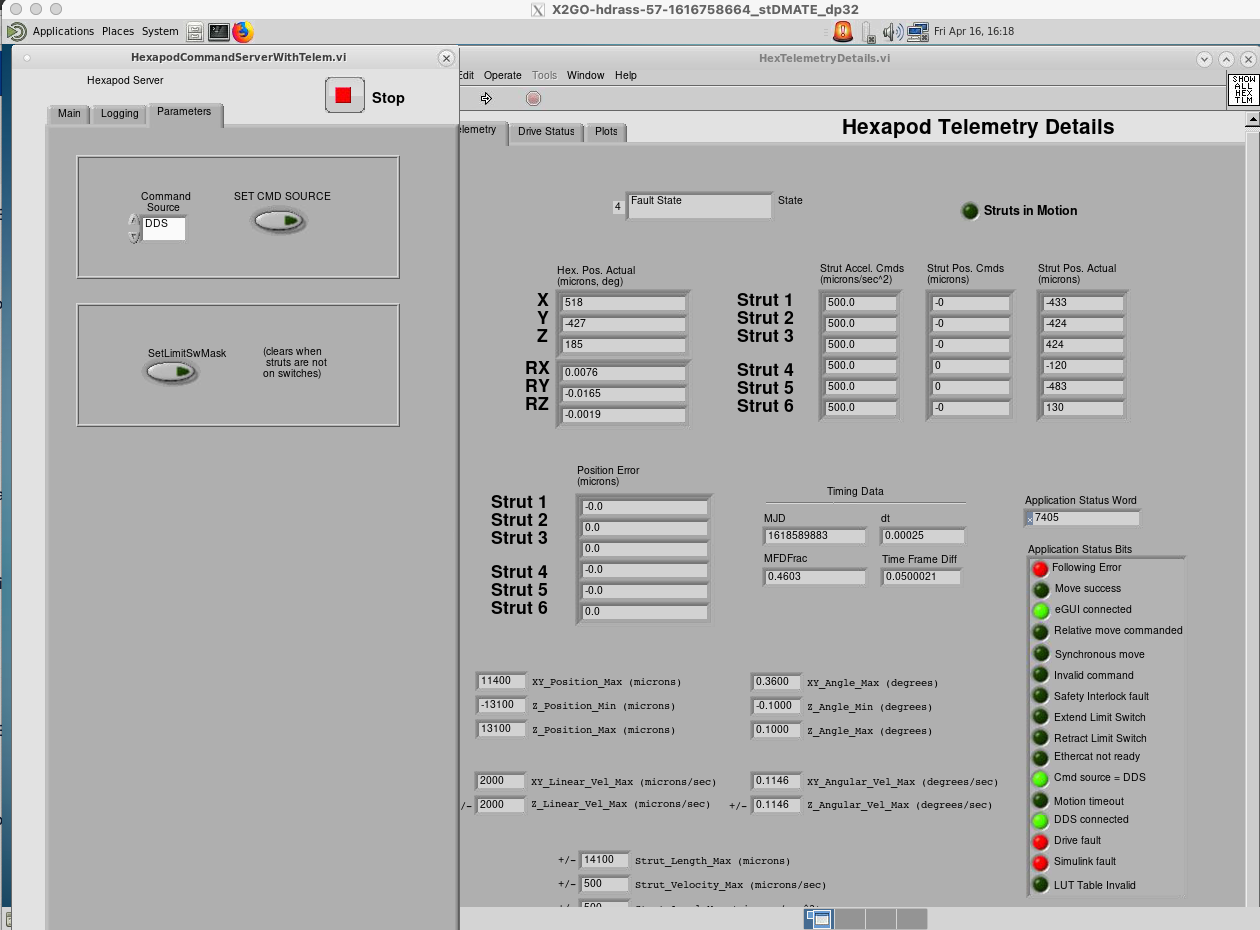
\includegraphics[width=3.12500in]{jira_imgs/1670.png}Hexapod stopped
after 1sec.

}
\begin{tabular}{p{2cm}p{14cm}}
\toprule
Step 51 & Step Execution Status: \textbf{ Fail } \\ \hline
\end{tabular}
 Description \\
{\footnotesize
Send the ``clearError'' trigger and bring the system to the
Enabled/Stationary state.

}
\hdashrule[0.5ex]{\textwidth}{1pt}{3mm}
  Expected Result \\
{\footnotesize
The system is in the Enabled/Stationary state and ready to be commanded.

}
\hdashrule[0.5ex]{\textwidth}{1pt}{3mm}
  Actual Result \\
{\footnotesize
Fault cleared, the system is in StandbyState.\\
Transitioned to enabled trough EUI\\
Entered into Enabled/MoivingPT-PT without hexapod movement.\\
Stop command send through EUI.\\
Status changed to enabled /stationary.\\[2\baselineskip]Moved back to
zero successfully.

}
\hdashrule[0.5ex]{\textwidth}{1pt}{3mm}
  Issues found executing this step:  \\
{\footnotesize
\begin{itemize}
\item \href{https://jira.lsstcorp.org/browse/DM-29792}{DM-29792}~~Camera Hexapod: The Enabled substate needs to be changed ``manually'' to
``clearError'' caused by unplugging the motor power cable.

\end{itemize}
}
\begin{tabular}{p{2cm}p{14cm}}
\toprule
Step 52 & Step Execution Status: \textbf{ Pass } \\ \hline
\end{tabular}
 Description \\
{\footnotesize
Activate an extension limit switch on one of the actuators by removing
the limit switch cover and manually tripping.~

}
\hdashrule[0.5ex]{\textwidth}{1pt}{3mm}
  Expected Result \\
{\footnotesize
An Extended Limit Switch error event is created and the system
transitions into Fault state.

}
\hdashrule[0.5ex]{\textwidth}{1pt}{3mm}
  Actual Result \\
{\footnotesize
Done by Felipe before.

}
\begin{tabular}{p{2cm}p{14cm}}
\toprule
Step 53 & Step Execution Status: \textbf{ Pass } \\ \hline
\end{tabular}
 Description \\
{\footnotesize
Send the ``clearError'' trigger and bring the system to the
Enabled/Stationary state.

}
\hdashrule[0.5ex]{\textwidth}{1pt}{3mm}
  Expected Result \\
{\footnotesize
The system is in the Enabled/Stationary state and ready to be commanded.

}
\hdashrule[0.5ex]{\textwidth}{1pt}{3mm}
  Actual Result \\
{\footnotesize
Done by Felipe before.

}
\begin{tabular}{p{2cm}p{14cm}}
\toprule
Step 54 & Step Execution Status: \textbf{ Pass } \\ \hline
\end{tabular}
 Description \\
{\footnotesize
Activate a retraction limit switch on one of the actuators by removing
the limit switch cover and manually tripping.

}
\hdashrule[0.5ex]{\textwidth}{1pt}{3mm}
  Expected Result \\
{\footnotesize
A Retracted Limit Switch error event is created and the system
transitions into Fault state.

}
\hdashrule[0.5ex]{\textwidth}{1pt}{3mm}
  Actual Result \\
{\footnotesize
Done by Felipe before.

}
\begin{tabular}{p{2cm}p{14cm}}
\toprule
Step 55 & Step Execution Status: \textbf{ Pass } \\ \hline
\end{tabular}
 Description \\
{\footnotesize
Send the ``clearError'' trigger and bring the system to the
Enabled/Stationary state.

}
\hdashrule[0.5ex]{\textwidth}{1pt}{3mm}
  Expected Result \\
{\footnotesize
The system is in the Enabled/Stationary state and ready to be commanded.

}
\hdashrule[0.5ex]{\textwidth}{1pt}{3mm}
  Actual Result \\
{\footnotesize
Done by Felipe before.

}
\begin{tabular}{p{2cm}p{14cm}}
\toprule
Step 56 & Step Execution Status: \textbf{ Fail } \\ \hline
\end{tabular}
 Description \\
{\footnotesize
Unplug the Ethercat cable between the control PC and the first Copley
XE2 drive.

}
\hdashrule[0.5ex]{\textwidth}{1pt}{3mm}
  Expected Result \\
{\footnotesize
An Ethercat Lost event is created and the system transitions to Fault
state.

}
\hdashrule[0.5ex]{\textwidth}{1pt}{3mm}
  Actual Result \\
{\footnotesize
The you EUI switched of without warning.\\
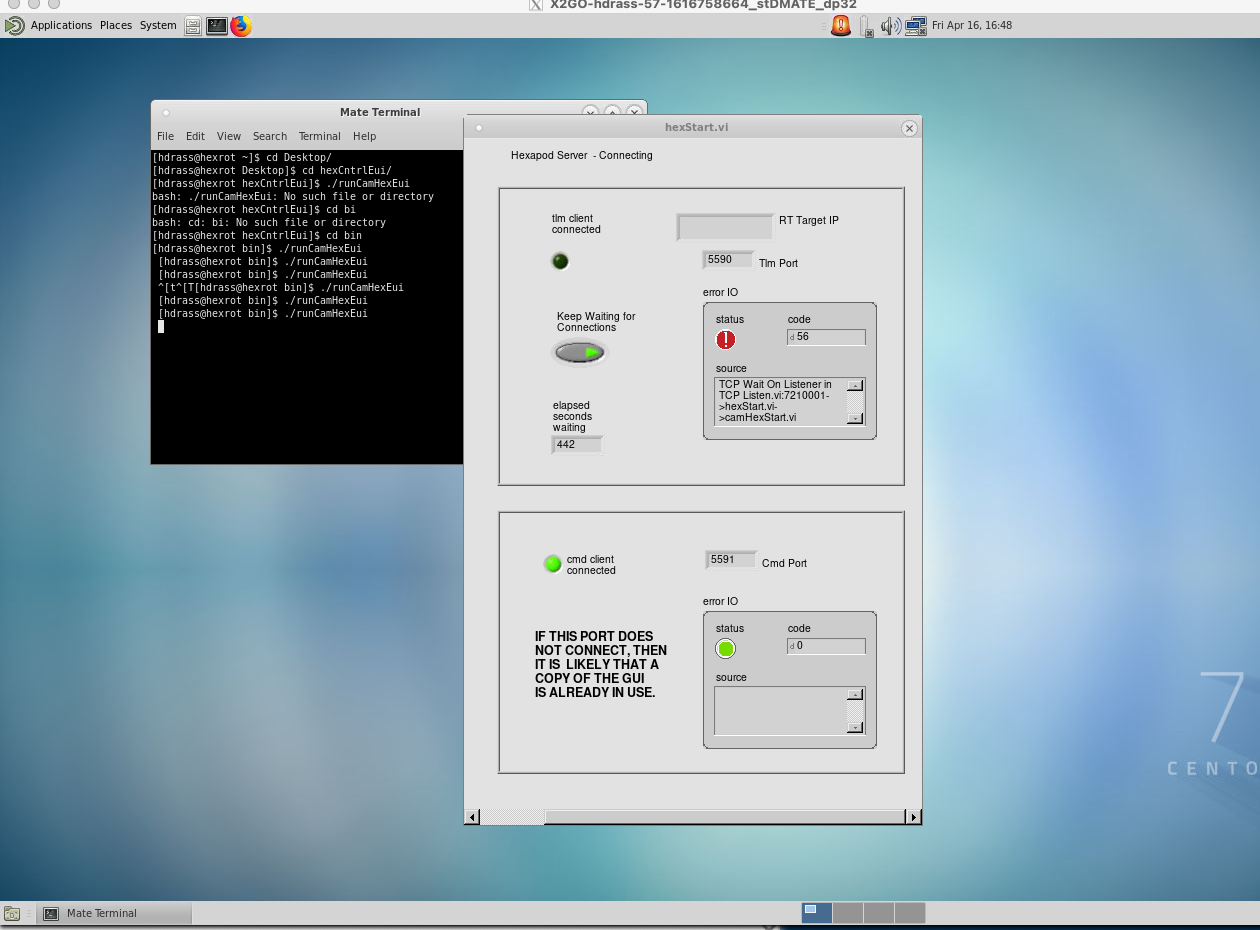
\includegraphics[width=3.12500in]{jira_imgs/1671.png}

}
\hdashrule[0.5ex]{\textwidth}{1pt}{3mm}
  Issues found executing this step:  \\
{\footnotesize
\begin{itemize}
\item \href{https://jira.lsstcorp.org/browse/DM-29793}{DM-29793}~~Camera Hexapod: The EUI needs to be restarted after re-plugging the
EtherCat cable

\end{itemize}
}
\begin{tabular}{p{2cm}p{14cm}}
\toprule
Step 57 & Step Execution Status: \textbf{ Not Executed } \\ \hline
\end{tabular}
 Description \\
{\footnotesize
Send the ``clearError'' trigger and bring the system to the
Enabled/Stationary state.

}
\hdashrule[0.5ex]{\textwidth}{1pt}{3mm}
  Expected Result \\
{\footnotesize
The system is in the Enabled/Stationary state and ready to be commanded.

}
\hdashrule[0.5ex]{\textwidth}{1pt}{3mm}
  Actual Result \\
{\footnotesize

}

\paragraph{ LVV-T1600 - Integration of Camera Hexapod with SAL 4.0 (LSST) }\mbox{}\\

Version \textbf{1}.
Open  \href{https://jira.lsstcorp.org/secure/Tests.jspa#/testCase/LVV-T1600}{\textit{ LVV-T1600 } }
test case in Jira.

The objective of this test case is to re-verify the functional
requirements of the camera hexapod's software, after shipment of the
hardware from the vendor's facility to the Summit, as defined in \citeds{LTS-206}
and \citeds{LTS-160}. This test case will only exercise the functionality that
was executed previously and meets the following criteria:

\begin{itemize}
\tightlist
\item
  Only requires the use of Russell's code to replace MOOG's middleware
  code
\item
  Only requires the camera hexapod to be operable
\item
  Only requires command through the CSC after the cRIO is switched from
  GUI mode to DDS mode
\item
  Only requires testing of the synchronous mode

  \begin{itemize}
  \tightlist
  \item
    \textbf{Asynchronous mode is not a standard mode of operation}
  \end{itemize}
\item
  Does \textbf{NOT} require the camera hexapod to be loaded with the
  camera simulated mass or actual camera hardware
\end{itemize}

The software functional requirements were previously verified during the
test campaign by the vendor at the vendor's facility and accepted by
LSST during the Factory Acceptance Test review. The test procedure used
during the vendor's acceptance testing is the \emph{LSST
Hexapods-Rotator Software Acceptance Test Procedure} which is attached
to this test case. The test steps of this test case are derived from the
same procedure, but the order of the steps have been changed to reflect
the \emph{Proposal of Hexapod Test~on Dec. 2019~}Confluence page which
can be found linked in the Traceability tab.\\[2\baselineskip]See the
attached \emph{LSST Rotator Hexapod's Manual} for more information on
how to operate the hexapod.

\textbf{ Preconditions}:\\
Prior to the execution of this test case to re-verify the Camera Hexapod
hardware functional requirements, the following Summit tasks must be
completed:

\begin{itemize}
\tightlist
\item
  The Hexapod has been installed on the camera cart

  \begin{itemize}
  \tightlist
  \item
    \url{https://jira.lsstcorp.org/browse/SUMMIT-3224}
  \end{itemize}
\item
  The Hexapod Controller has been deployed on the summit

  \begin{itemize}
  \tightlist
  \item
    \url{https://jira.lsstcorp.org/browse/SUMMIT-3229}
  \end{itemize}
\item
  Boxes for the Hexapod have been transported to the 3rd level

  \begin{itemize}
  \tightlist
  \item
    \url{https://jira.lsstcorp.org/browse/SUMMIT-3230}
  \end{itemize}
\item
  All Hexapod cables and cabinets have been prepared for integration
  with camera cart

  \begin{itemize}
  \tightlist
  \item
    \url{https://jira.lsstcorp.org/browse/SUMMIT-3231}
  \end{itemize}
\item
  The offset has been installed onto the integrating structure

  \begin{itemize}
  \tightlist
  \item
    \url{https://jira.lsstcorp.org/browse/SUMMIT-3293}
  \end{itemize}
\item
  The Camera Hexapod electrical connections have been tested

  \begin{itemize}
  \tightlist
  \item
    \url{https://jira.lsstcorp.org/browse/SUMMIT-3294}
  \end{itemize}
\end{itemize}

Execution status: {\bf Fail }

Final comment:\\

Issues found during the execution of LVV-T1600 test case:

\begin{itemize}
\item \href{https://jira.lsstcorp.org/browse/DM-29550}{DM-29550}~~ControlledStop event

\item \href{https://jira.lsstcorp.org/browse/DM-29692}{DM-29692}~~Camera MThexapod CompensationMode does not work

\item \href{https://jira.lsstcorp.org/browse/DM-29689}{DM-29689}~~Camera MThexapod inPosition event not generated

\item \href{https://jira.lsstcorp.org/browse/DM-29693}{DM-29693}~~Pivot changes are not reported in the EUI and the EFD.

\item \href{https://jira.lsstcorp.org/browse/DM-29705}{DM-29705}~~Camera hexapod state machine does not transition back to StandbyState

\item \href{https://jira.lsstcorp.org/browse/DM-29706}{DM-29706}~~Disable command accepted but state machine did not change status

\end{itemize}

Detailed steps results:

\begin{tabular}{p{2cm}p{14cm}}
\toprule
Step 1 & Step Execution Status: \textbf{ Pass } \\ \hline
\end{tabular}
 Description \\
{\footnotesize
\textbf{STARTING THE EUI}\\[2\baselineskip]Double click the Hexapod GUI
Viewer desktop icon on the computer.

\begin{itemize}
\tightlist
\item
  This can be done on the Dell Management PC or another computer on the
  same network
\end{itemize}

}
\hdashrule[0.5ex]{\textwidth}{1pt}{3mm}
  Expected Result \\
{\footnotesize
A prompt to enter a password is shown.~

}
\hdashrule[0.5ex]{\textwidth}{1pt}{3mm}
  Actual Result \\
{\footnotesize
Starting the EUI is done through X2GO and the terminal.\\
Ask IT to set it up for you and copy the EUI scripts in the latest
version on your account.\\
CAVE: The logic of the limit switches changed. Only the latest version
EUI version is working.\\
Use your personalized X2GO account to connect to hexrot.cp.lsst.org\\
Use your personalized IPA password to login into your account.\\
Open a terminal. Change the past to
\textasciitilde{}/Desktop/hexCntrlEui/bin\\
Start the EUI with: ./runCamHexEui\\[2\baselineskip]

}
\begin{tabular}{p{2cm}p{14cm}}
\toprule
Step 2 & Step Execution Status: \textbf{ Pass } \\ \hline
\end{tabular}
 Description \\
{\footnotesize
Enter the password ``lsst-vnc''

\begin{itemize}
\tightlist
\item
  If the EUI isn't automatically up and running when the VNC opens,
  double click on the Hexapod-eGUI icon on the VNC viewer
\end{itemize}

}
\hdashrule[0.5ex]{\textwidth}{1pt}{3mm}
  Expected Result \\
{\footnotesize
The EUI is in the Offline State/PublishOnly substate and is able to
publish through SAL but cannot receive commands.

}
\hdashrule[0.5ex]{\textwidth}{1pt}{3mm}
  Actual Result \\
{\footnotesize
Included in the previous step.

}
\begin{tabular}{p{2cm}p{14cm}}
\toprule
Step 3 & Step Execution Status: \textbf{ Pass } \\ \hline
\end{tabular}
 Description \\
{\footnotesize
\textbf{OFFLINESTATE/PUBLISHONLY -\textgreater{}
OFFLINESTATE/AVAILABLESTATE}\\
On the Main tab, select the ``Offline SubState Cmd'' field in the
Commands to Send section, set the Offline SubState Triggers to ``System
Ready'' and click on the Send Command button.\\
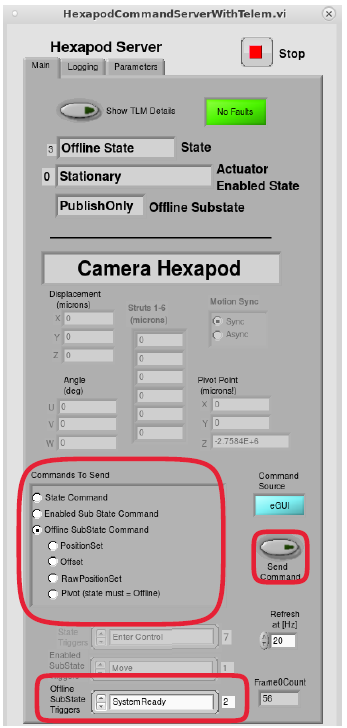
\includegraphics[width=1.79167in]{jira_imgs/1024.png}

}
\hdashrule[0.5ex]{\textwidth}{1pt}{3mm}
  Expected Result \\
{\footnotesize
The system transitions from the OfflineState/PublishOnly substate to the
OfflineState/AvailableState substate.\\[2\baselineskip]

}
\hdashrule[0.5ex]{\textwidth}{1pt}{3mm}
  Actual Result \\
{\footnotesize
Substate changes as expected.

}
\begin{tabular}{p{2cm}p{14cm}}
\toprule
Step 4 & Step Execution Status: \textbf{ Pass } \\ \hline
\end{tabular}
 Description \\
{\footnotesize
\textbf{SWITCHING TO DDS MODE}\\
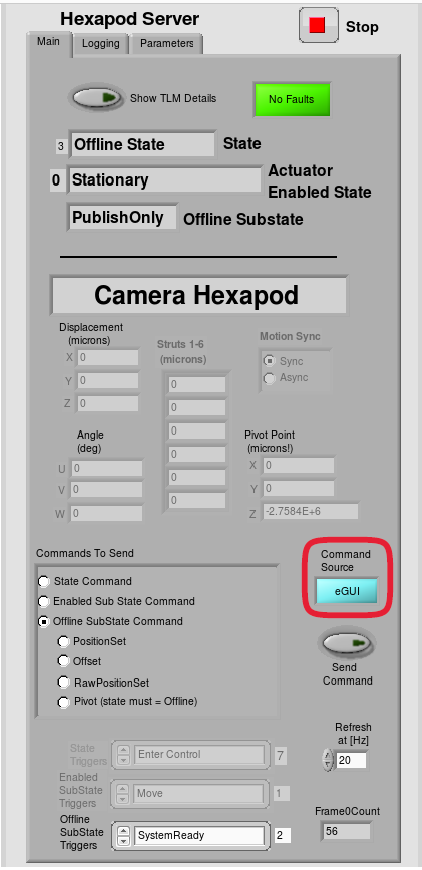
\includegraphics[width=1.68750in]{jira_imgs/1025.png}If the Command
Source does not show DDS, go to the Parameters tab, select DDS under the
Command Source and click the Set Cmd Source button.\\
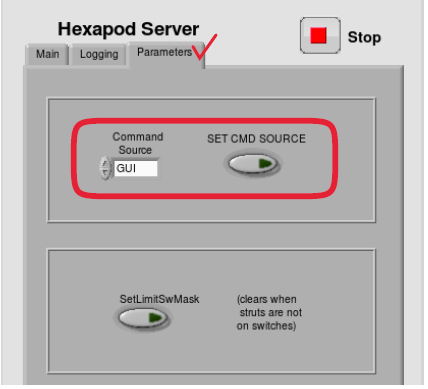
\includegraphics[width=2.34375in]{jira_imgs/1026.png}\textbf{Note:~If
the GUI is used after being set to DDS mode, the system will switch back
the Command Source to GUI and ignore any DDS commands. The Command
Source must show DDS in order to receive DDS commands.}

}
\hdashrule[0.5ex]{\textwidth}{1pt}{3mm}
  Expected Result \\
{\footnotesize
The system is capable of receiving/responding to DDS commands.

}
\hdashrule[0.5ex]{\textwidth}{1pt}{3mm}
  Actual Result \\
{\footnotesize
Control mode changes as expected. Note confirmed. Any command from the
EUI changes the control back to the EUI. This must manually be changed
to give control back to the DDS.

}
\begin{tabular}{p{2cm}p{14cm}}
\toprule
Step 5 & Step Execution Status: \textbf{ Pass } \\ \hline
\end{tabular}
 Description \\
{\footnotesize
\textbf{OFFLINESTATE -\textgreater{} STANDBYSTATE}\\
The system receives an enterControl State Transition command through
DDS.

}
\hdashrule[0.5ex]{\textwidth}{1pt}{3mm}
  Expected Result \\
{\footnotesize
The system transitions into the StandbyState and is capable of
receiving/responding to DDS commands.

}
\hdashrule[0.5ex]{\textwidth}{1pt}{3mm}
  Actual Result \\
{\footnotesize
State changes as expected.

}
\begin{tabular}{p{2cm}p{14cm}}
\toprule
Step 6 & Step Execution Status: \textbf{ Pass } \\ \hline
\end{tabular}
 Description \\
{\footnotesize
\textbf{STANDBYSTATE -\textgreater{} DISABLEDSTATE}\\
From the StandbyState, send a start command through the DDS.

}
\hdashrule[0.5ex]{\textwidth}{1pt}{3mm}
  Expected Result \\
{\footnotesize
The system transitions into DisabledState after receiving/responding to
DDS command and the wrapper in the PXI real time controller looks for
the configuration file.\\[2\baselineskip]If the configuration file is
invalid or out of range, the system will transition into a Fault State

}
\hdashrule[0.5ex]{\textwidth}{1pt}{3mm}
  Actual Result \\
{\footnotesize
Here the range of the parameters in the configuration file.\\
This is working. State machine transitioned from StandbyState to
DisableState without faulting.

}
\begin{tabular}{p{2cm}p{14cm}}
\toprule
Step 7 & Step Execution Status: \textbf{ Pass } \\ \hline
\end{tabular}
 Description \\
{\footnotesize
\textbf{DISABLEDSTATE -\textgreater{} ENABLEDSTATE}\\
From the DisabledState, send an enable state command through the DDS.\\
\textbf{}

}
\hdashrule[0.5ex]{\textwidth}{1pt}{3mm}
  Expected Result \\
{\footnotesize
The system transitions into the EnabledState/Stationary substate, the
motor drives are enabled, motor brakes are released and the system is
capable of receiving/responding to DDS commands.\\[2\baselineskip]

}
\hdashrule[0.5ex]{\textwidth}{1pt}{3mm}
  Actual Result \\
{\footnotesize
Substate changes as expected.\\
Motor drives are enabled.\\
\textbf{Not sure if there are motor breaks. But if there are motor
breaks they are released.}\\
The system is capable of receiving/responding to DDS
commands.\\[2\baselineskip]

}
\begin{tabular}{p{2cm}p{14cm}}
\toprule
Step 8 & Step Execution Status: \textbf{ Pass w/ Deviation } \\ \hline
\end{tabular}
 Description \\
{\footnotesize
\textbf{FAULTSTATE}\\
If a Fault occurs in any of the other states, the system will
automatically transition to the Fault State. While in the Fault state,
send a clearError command through the DDS.\\
Note: If the fault that occurs goes through the interlock system, reset
the safety relay switch and send a clearError command.

}
\hdashrule[0.5ex]{\textwidth}{1pt}{3mm}
  Expected Result \\
{\footnotesize
The system transitions back to the OfflineState/PublishOnly substate and
is not capable of receiving/responding to DDS commands. (Go back to Step
3)

}
\hdashrule[0.5ex]{\textwidth}{1pt}{3mm}
  Actual Result \\
{\footnotesize
Yes, the system goes to FaultState when a fault occurs in one of the
other states.\\[2\baselineskip]Yes, the FaultState can be cleared by
sending a clearError command through the DDS if the fault condition does
not exist anymore.\\[2\baselineskip]Deviation: The system transitions
back to StandbyState and can be commanded from DDS again. No need to go
back to step 3.

}
\begin{tabular}{p{2cm}p{14cm}}
\toprule
Step 9 & Step Execution Status: \textbf{ Pass } \\ \hline
\end{tabular}
 Description \\
{\footnotesize
Verify that the thermal sensors are connected and producing telemetry
into the EFD.

}
\hdashrule[0.5ex]{\textwidth}{1pt}{3mm}
  Expected Result \\
{\footnotesize
All actuator temperatures are published to the EFD.

}
\hdashrule[0.5ex]{\textwidth}{1pt}{3mm}
  Actual Result \\
{\footnotesize
Deviation: The thermal sensors were not available at the moment of the
tests.\\
The Tests were executed without the thermal sensors.\\
A waiting time of 39 sec was added after each movement.\\
This time is comparable to the time between two hexapod movements in
operations.

}
\begin{tabular}{p{2cm}p{14cm}}
\toprule
Step 10 & Step Execution Status: \textbf{ Pass } \\ \hline
\end{tabular}
 Description \\
{\footnotesize
The following steps define what the Jupyter Notebook for this test case
implements. Executing the Jupyter notebook is the only actual command
and control step that needs to be executed.

}
\hdashrule[0.5ex]{\textwidth}{1pt}{3mm}
  Expected Result \\
{\footnotesize
The Jupyter notebook controls the system to run through the steps below.

}
\hdashrule[0.5ex]{\textwidth}{1pt}{3mm}
  Actual Result \\
{\footnotesize
Yes, the tests here were executed using the notebooks:\\
https://github.com/lsst-ts/ts\_notebooks/blob/origin/tickets/SE-1372/procedures/lvv-t1600.ipynb\\
and for the compensationMode tests:\\
https://github.com/lsst-ts/ts\_notebooks/blob/origin/tickets/SE-1372/bxin/ptg2hex/hex\_diagnostics.ipynb

}
\begin{tabular}{p{2cm}p{14cm}}
\toprule
Step 11 & Step Execution Status: \textbf{ Pass } \\ \hline
\end{tabular}
 Description \\
{\footnotesize
Verify all the telemetry is being ingested into the EFD.

}
\hdashrule[0.5ex]{\textwidth}{1pt}{3mm}
  Expected Result \\
{\footnotesize
All telemetry defined in the script is being ingested into the EFD.

}
\hdashrule[0.5ex]{\textwidth}{1pt}{3mm}
  Actual Result \\
{\footnotesize
To make sure that the telemetry is ingested into the EFD a test message
was sent to the EFD and read from Chronograph:\\

\begin{longtable}[]{@{}lll@{}}
\toprule
\begin{minipage}[t]{0.32\columnwidth}\raggedright\strut
time\\
\strut
\end{minipage} & \begin{minipage}[t]{0.32\columnwidth}\raggedright\strut
lsst.sal.Script.logevent\_logMessage.ScriptID\strut
\end{minipage} & \begin{minipage}[t]{0.32\columnwidth}\raggedright\strut
lsst.sal.Script.logevent\_logMessage.message\strut
\end{minipage}\tabularnewline
\begin{minipage}[t]{0.30\columnwidth}\raggedright\strut
03/25/2021 12:41:12\\
\strut
\end{minipage} & \begin{minipage}[t]{0.30\columnwidth}\raggedright\strut
42658886.00\\
\strut
\end{minipage} & \begin{minipage}[t]{0.30\columnwidth}\raggedright\strut
TEST to see if annotations like this arrive in the EFD.\\
\strut
\end{minipage}\tabularnewline
\bottomrule
\end{longtable}

}
\begin{tabular}{p{2cm}p{14cm}}
\toprule
Step 12 & Step Execution Status: \textbf{ Pass } \\ \hline
\end{tabular}
 Description \\
{\footnotesize
\textbf{{MOVE TEST}}\\
\textbf{Section 3.1.2 of the attached Software Acceptance Test
Procedure\\
Test Sequence \#1 - Synchronous PositionSet and Move Commands}\\
In enabled/stationary state, send a positionSet command of (0um, 0um,
200um, 0 deg, 0 deg, 0 deg, s).

}
\hdashrule[0.5ex]{\textwidth}{1pt}{3mm}
  Test Data \\
 {\footnotesize
\textbf{Deviation:~}Skip this step. positionSet and move command
replaced by new move command. Now, the hexapod starts movement directly
after receiving the command.

}
\hdashrule[0.5ex]{\textwidth}{1pt}{3mm}
  Expected Result \\
{\footnotesize
The hexapod does not move.

}
\hdashrule[0.5ex]{\textwidth}{1pt}{3mm}
  Actual Result \\
{\footnotesize

}
\begin{tabular}{p{2cm}p{14cm}}
\toprule
Step 13 & Step Execution Status: \textbf{ Pass } \\ \hline
\end{tabular}
 Description \\
{\footnotesize
With the synchronous button enabled and in enabled/stationary state,
send a positionSet command of (500um, -500um, 200um, 0.01deg, -0.015deg,
0deg).

}
\hdashrule[0.5ex]{\textwidth}{1pt}{3mm}
  Test Data \\
 {\footnotesize
\textbf{Deviation:~}Skip this step. positionSet and move command
replaced by new move command. Now, the hexapod starts movement directly
after receiving the command.

}
\hdashrule[0.5ex]{\textwidth}{1pt}{3mm}
  Expected Result \\
{\footnotesize
The hexapod does not move

}
\hdashrule[0.5ex]{\textwidth}{1pt}{3mm}
  Actual Result \\
{\footnotesize

}
\begin{tabular}{p{2cm}p{14cm}}
\toprule
Step 14 & Step Execution Status: \textbf{ Pass } \\ \hline
\end{tabular}
 Description \\
{\footnotesize
With the hexapod in in enabled/stationary state sync=True and send the
move command of (x= 500um,y= -500um, z=200um, u=0.01deg, v=-0.015deg,
w=0deg).

}
\hdashrule[0.5ex]{\textwidth}{1pt}{3mm}
  Expected Result \\
{\footnotesize
\begin{itemize}
\tightlist
\item
  The hexapod moves to (x= 500um,y= -500um, z=200um, u=0.01deg,
  v=-0.015deg, w=0deg)
\item
  Since the Hexapod is in synchronous mode, the actuators complete the
  move at nearly the same time.
\end{itemize}

}
\hdashrule[0.5ex]{\textwidth}{1pt}{3mm}
  Actual Result \\
{\footnotesize
The hexapod moved to the expected position and the results read from the
EFD are:\\[2\baselineskip]

\begin{verbatim}
INFO:Script:STOP- Camera Hexapod Integration Test -- LVV-T1600 Test Step 7
\end{verbatim}

\begin{verbatim}
hex position
    500.05     -500.87      200.12        0.01       -0.01       -0.00  
\end{verbatim}

}
\begin{tabular}{p{2cm}p{14cm}}
\toprule
Step 15 & Step Execution Status: \textbf{ Fail } \\ \hline
\end{tabular}
 Description \\
{\footnotesize
Record the corresponding DDS events that were generated.

}
\hdashrule[0.5ex]{\textwidth}{1pt}{3mm}
  Expected Result \\
{\footnotesize
\begin{itemize}
\tightlist
\item
  The controllerState.enabledSubstate goes to MOVING\_POINT\_TO\_POINT
  when the move begins and STATIONARY when the move ends.
\item
  An inPosition event is generated when the move is complete
\end{itemize}

}
\hdashrule[0.5ex]{\textwidth}{1pt}{3mm}
  Actual Result \\
{\footnotesize
Yes, the controllerState.enabledSubstate goes to
MOVING\_POINT\_TO\_POINT when the move begins and STATIONARY when the
move ends.\\[2\baselineskip]The inPosition event was not generated.\\
Looking at the EFD, the EFD shows that only for actuator one a status is
present.\\
Actuators 2-6 always present the status zero.\\
Assuming that the information from all six actuators is needed, the
inPosition event is not generated because of missing information on
actuators 2-6.\\[2\baselineskip]

}
\hdashrule[0.5ex]{\textwidth}{1pt}{3mm}
  Issues found executing this step:  \\
{\footnotesize
\begin{itemize}
\item \href{https://jira.lsstcorp.org/browse/DM-29689}{DM-29689}~~Camera MThexapod inPosition event not generated

\end{itemize}
}
\begin{tabular}{p{2cm}p{14cm}}
\toprule
Step 16 & Step Execution Status: \textbf{ Pass } \\ \hline
\end{tabular}
 Description \\
{\footnotesize
Wait 39 seconds.

}
\hdashrule[0.5ex]{\textwidth}{1pt}{3mm}
  Expected Result \\
{\footnotesize

}
\hdashrule[0.5ex]{\textwidth}{1pt}{3mm}
  Actual Result \\
{\footnotesize

}
\begin{tabular}{p{2cm}p{14cm}}
\toprule
Step 17 & Step Execution Status: \textbf{ Pass } \\ \hline
\end{tabular}
 Description \\
{\footnotesize
Record the corresponding thermal sensors and verify they are below 19
deg C. If they are above 19 deg C, wait until they are below 19 deg C to
perform the following steps.

}
\hdashrule[0.5ex]{\textwidth}{1pt}{3mm}
  Expected Result \\
{\footnotesize
All actuators are below 19 deg C.

}
\hdashrule[0.5ex]{\textwidth}{1pt}{3mm}
  Actual Result \\
{\footnotesize
Thermal sensors were not present during the tests. See step 9.

}
\begin{tabular}{p{2cm}p{14cm}}
\toprule
Step 18 & Step Execution Status: \textbf{ Pass } \\ \hline
\end{tabular}
 Description \\
{\footnotesize
\textbf{Section 3.1.2 of the attached Software Acceptance Test
Procedure\\
Test Sequence \#5 - Stop Commands}\\
In the enabled/stationary state, send a move command of (x=0um, y=0um,
z=5000um, u=0deg, v=0deg, w=0deg)

}
\hdashrule[0.5ex]{\textwidth}{1pt}{3mm}
  Expected Result \\
{\footnotesize
The hexapod doesn't move.

}
\hdashrule[0.5ex]{\textwidth}{1pt}{3mm}
  Actual Result \\
{\footnotesize
Deviation: With the modified move command it is expected that the
hexapod moves during the step to (x=0um, y=0um, z=5000um, u=0deg,
v=0deg, w=0deg).\\
When executing the move the hexapod started to moved and the movement
was correctly reflected in the EFD.

}
\begin{tabular}{p{2cm}p{14cm}}
\toprule
Step 19 & Step Execution Status: \textbf{ Pass } \\ \hline
\end{tabular}
 Description \\
{\footnotesize
Wait 3s.

}
\hdashrule[0.5ex]{\textwidth}{1pt}{3mm}
  Expected Result \\
{\footnotesize

}
\hdashrule[0.5ex]{\textwidth}{1pt}{3mm}
  Actual Result \\
{\footnotesize

}
\begin{tabular}{p{2cm}p{14cm}}
\toprule
Step 20 & Step Execution Status: \textbf{ Pass } \\ \hline
\end{tabular}
 Description \\
{\footnotesize
Send a stop command.

}
\hdashrule[0.5ex]{\textwidth}{1pt}{3mm}
  Expected Result \\
{\footnotesize
The hexapod stops before reaching the previously commanded position

}
\hdashrule[0.5ex]{\textwidth}{1pt}{3mm}
  Actual Result \\
{\footnotesize
Yes, the hexapod stopped at the following position:\\[2\baselineskip]

\begin{verbatim}
INFO:Script:STOP- Camera Hexapod Integration Test -- LVV-T1600 Test Step 11
\end{verbatim}

\begin{verbatim}
hex position
      0.38       -1.13    -1503.11       -0.00       -0.00        0.00  
\end{verbatim}

}
\begin{tabular}{p{2cm}p{14cm}}
\toprule
Step 21 & Step Execution Status: \textbf{ Fail } \\ \hline
\end{tabular}
 Description \\
{\footnotesize
Record the corresponding DDS events that were generated.

}
\hdashrule[0.5ex]{\textwidth}{1pt}{3mm}
  Expected Result \\
{\footnotesize
\begin{itemize}
\tightlist
\item
  The controllerState.enabledSubstate goes to CONTROLLED\_STOPPING when
  the stop is requested, then STATIONARY when the hexapod has halted.
\item
  In the EFD the codes for the EnabledSubstate are:

  \begin{itemize}
  \tightlist
  \item
    Stationary=0
  \item
    MovingPointToPoint=1
  \item
    SlewingOrTracking=2
  \item
    ControlledStopping=3
  \item
    Initializing=4
  \item
    Relative=5
  \item
    ConstantVelocity=6
  \end{itemize}
\item
  No inPosition event is generated.
\end{itemize}

}
\hdashrule[0.5ex]{\textwidth}{1pt}{3mm}
  Actual Result \\
{\footnotesize
Fail: There is no ControlledStopping event shown in the EFD under
controllerState.enabledSubstate.

}
\hdashrule[0.5ex]{\textwidth}{1pt}{3mm}
  Issues found executing this step:  \\
{\footnotesize
\begin{itemize}
\item \href{https://jira.lsstcorp.org/browse/DM-29550}{DM-29550}~~ControlledStop event

\end{itemize}
}
\begin{tabular}{p{2cm}p{14cm}}
\toprule
Step 22 & Step Execution Status: \textbf{ Pass } \\ \hline
\end{tabular}
 Description \\
{\footnotesize
Wait 39 seconds.

}
\hdashrule[0.5ex]{\textwidth}{1pt}{3mm}
  Expected Result \\
{\footnotesize

}
\hdashrule[0.5ex]{\textwidth}{1pt}{3mm}
  Actual Result \\
{\footnotesize

}
\begin{tabular}{p{2cm}p{14cm}}
\toprule
Step 23 & Step Execution Status: \textbf{ Pass } \\ \hline
\end{tabular}
 Description \\
{\footnotesize
Record the corresponding thermal sensors and verify they are below 19
deg C. If they are above 19 deg C, wait until they are below 19 deg C to
perform the following steps.

}
\hdashrule[0.5ex]{\textwidth}{1pt}{3mm}
  Expected Result \\
{\footnotesize
All actuators are below 19 deg C.

}
\hdashrule[0.5ex]{\textwidth}{1pt}{3mm}
  Actual Result \\
{\footnotesize
Thermal sensors were not present during the tests. See step 9.

}
\begin{tabular}{p{2cm}p{14cm}}
\toprule
Step 24 & Step Execution Status: \textbf{ Pass w/ Deviation } \\ \hline
\end{tabular}
 Description \\
{\footnotesize
\textbf{Section 3.1.2 of the attached Software Acceptance Test
Procedure\\
Test Sequence \#9 - positionSet and
moveLUT}\\[2\baselineskip]\textbf{Update: Test the
``setCompensationMode'' command.}\\[2\baselineskip]In enabled/stationary
state, send a move command of (x=0um, y=0um, z=800um, u=0deg, v=0deg,
w=0deg)\\[2\baselineskip]

}
\hdashrule[0.5ex]{\textwidth}{1pt}{3mm}
  Test Data \\
 {\footnotesize
\textbf{Deviation:} There is no ``positionSet'' and no ``moveLUT''
command anymore. ``positionSet'' and ``move'' command replaced by new
``move'' command. Now, the hexapod starts movement directly after
receiving the command. moveLUT is replaced by a ``setCompensationMode''.

}
\hdashrule[0.5ex]{\textwidth}{1pt}{3mm}
  Expected Result \\
{\footnotesize
The hexapod moves to the position (x=0um, y=0um, z=800um, u=0deg,
v=0deg, w=0deg) and, since we are moving in synchronous mode, the
actuators complete the move at nearly the same time.

}
\hdashrule[0.5ex]{\textwidth}{1pt}{3mm}
  Actual Result \\
{\footnotesize
The test is executed using the notebook:\\
https://github.com/lsst-ts/ts\_notebooks/blob/origin/tickets/SE-1372/bxin/ptg2hex/hex\_diagnostics.ipynb\\
Original results can be found in this notebook.\\
Deviation: The hexapod is sent to and arrived at\\

\begin{verbatim}
Current Hexapod position
     -0.74       0.03    -250.21       0.00       0.00      -0.00
\end{verbatim}

}
\begin{tabular}{p{2cm}p{14cm}}
\toprule
Step 25 & Step Execution Status: \textbf{ Pass w/ Deviation } \\ \hline
\end{tabular}
 Description \\
{\footnotesize
Ensure that MTMount publishes the telescope elevation angle and
MTRotator publishes the rotation angle of the rotator. Either as real
components or through controllers simulating the components.

}
\hdashrule[0.5ex]{\textwidth}{1pt}{3mm}
  Expected Result \\
{\footnotesize
Published telescope elevation and rotator angle.

}
\hdashrule[0.5ex]{\textwidth}{1pt}{3mm}
  Actual Result \\
{\footnotesize
Deviation: MTHexapod also expects MTMount azimuth.\\
The real MTRotator component is publishing its angle at
``lsst.sal.MTRotator.rotation.mean\_actualPosition''.\\
The MTMount elevation and azimuth are published by a controller
simulating the MTMount telemetry at
``lsst.sal.MTMount.elevation.actualPosition'' and
``lsst.sal.MTMount.azimuth.actualPosition''

}
\begin{tabular}{p{2cm}p{14cm}}
\toprule
Step 26 & Step Execution Status: \textbf{ Pass } \\ \hline
\end{tabular}
 Description \\
{\footnotesize
In enabled/stationary state, set ~``setCompensationMode'' command to
enable=True.

}
\hdashrule[0.5ex]{\textwidth}{1pt}{3mm}
  Expected Result \\
{\footnotesize
The hexapod does not move and the
~MTHexapod.command\_setCompensationMode appears as true in the
EFD.\\[2\baselineskip]logevent\_compensatedPosition is sent to the
EFD.\\[2\baselineskip]

}
\hdashrule[0.5ex]{\textwidth}{1pt}{3mm}
  Actual Result \\
{\footnotesize
EFD:\\[2\baselineskip]START- Camera Hexapod Integration Test --
LVV-T1600 Compensation mode test Step 17- Starting time: 2021-03-25
15:51:28.133715 UTC\\[2\baselineskip]START- Camera Hexapod Integration
Test -- LVV-T1600 Compensation mode test Step 17- Starting time:
2021-03-25 17:43:19.848705 UTC\\[2\baselineskip]STOP - 18:09
UTC\\[2\baselineskip]The MTHexapod.command\_setCompensationMode event is
generated and can be read from the EFD.\\[2\baselineskip]Once the
setCompensationMode=true for the first time the logevents:
``MTHexapod.logevent\_uncompensatedPosition'' and
``MTHexapod.logevent\_compensatedPosition'' appear both to all the time
in the EFD until about 1h after setCompensationMode=false.

}
\begin{tabular}{p{2cm}p{14cm}}
\toprule
Step 27 & Step Execution Status: \textbf{ Fail } \\ \hline
\end{tabular}
 Description \\
{\footnotesize
In enabled/stationary state, send a move command of (0um, 0um, 800um,
0deg, 0deg, 0deg)

}
\hdashrule[0.5ex]{\textwidth}{1pt}{3mm}
  Expected Result \\
{\footnotesize
The hexapod moves to a slightly different position than (0um, 0um,
800um, 0deg, 0deg, 0deg) and, since we are moving in synchronous mode,
the actuators complete the move at nearly the same time.

}
\hdashrule[0.5ex]{\textwidth}{1pt}{3mm}
  Actual Result \\
{\footnotesize
Deviation: Move command to (0um, 0um, -250um, 0deg, 0deg, 0deg) send.\\
Failure: The move command was rejected.\\
When entering compensationMode the EUI keeps switching between
Stationary and Moving Pt-Pt.\\
EFD is reflecting this under
``MTHexapod.logevent\_controllerState.enabledSubstate''\\
Cause:\\
Does this happens because actuators 2-6 do not report their position
---\textgreater{} inPosition event is not generated ---\textgreater{}
compensationMode keeps compensating ---\textgreater{} hexapod does not
accept further move command because it is constantly ``moving''?

}
\hdashrule[0.5ex]{\textwidth}{1pt}{3mm}
  Issues found executing this step:  \\
{\footnotesize
\begin{itemize}
\item \href{https://jira.lsstcorp.org/browse/DM-29692}{DM-29692}~~Camera MThexapod CompensationMode does not work

\end{itemize}
}
\begin{tabular}{p{2cm}p{14cm}}
\toprule
Step 28 & Step Execution Status: \textbf{ Blocked } \\ \hline
\end{tabular}
 Description \\
{\footnotesize
Check if there are any different events between move with and without
setCompensationMode=True. Check the movement in the EFD use:\\
Compare logevent\_compensatedPosition to logevent\_uncompensatedPosition

}
\hdashrule[0.5ex]{\textwidth}{1pt}{3mm}
  Expected Result \\
{\footnotesize
The changes are expected according to this table:\\
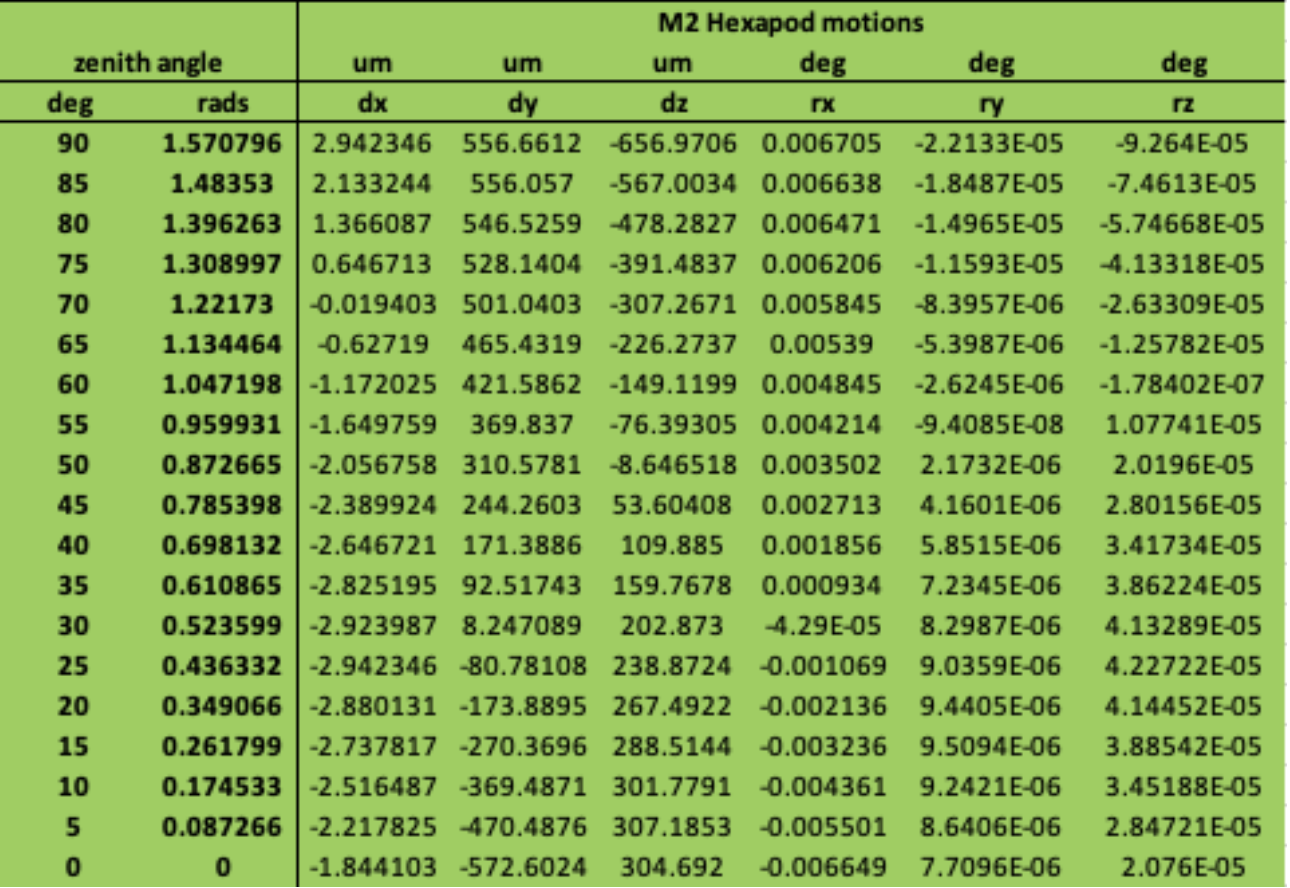
\includegraphics[width=1.56250in]{jira_imgs/1620.png}\\

}
\hdashrule[0.5ex]{\textwidth}{1pt}{3mm}
  Actual Result \\
{\footnotesize
Not tested: Hexapod is not compensating see previous
step.\\[2\baselineskip]

}
\begin{tabular}{p{2cm}p{14cm}}
\toprule
Step 29 & Step Execution Status: \textbf{ Blocked } \\ \hline
\end{tabular}
 Description \\
{\footnotesize
In enabled/stationary state, send a move command of (0um, 0um, 800um,
0deg, 0deg, 0deg)

}
\hdashrule[0.5ex]{\textwidth}{1pt}{3mm}
  Expected Result \\
{\footnotesize
The hexapod does not move since it stayed in compensationMode.

}
\hdashrule[0.5ex]{\textwidth}{1pt}{3mm}
  Actual Result \\
{\footnotesize
Not tested: Hexapod is not compensating see previous step.

}
\begin{tabular}{p{2cm}p{14cm}}
\toprule
Step 30 & Step Execution Status: \textbf{ Pass } \\ \hline
\end{tabular}
 Description \\
{\footnotesize
Wait 39 seconds.

}
\hdashrule[0.5ex]{\textwidth}{1pt}{3mm}
  Expected Result \\
{\footnotesize

}
\hdashrule[0.5ex]{\textwidth}{1pt}{3mm}
  Actual Result \\
{\footnotesize

}
\begin{tabular}{p{2cm}p{14cm}}
\toprule
Step 31 & Step Execution Status: \textbf{ Pass } \\ \hline
\end{tabular}
 Description \\
{\footnotesize
Record the corresponding thermal sensors and verify they are below 19
deg C. If they are above 19 deg C, wait until they are below 19 deg C to
perform the following steps.

}
\hdashrule[0.5ex]{\textwidth}{1pt}{3mm}
  Expected Result \\
{\footnotesize
All actuators are below 19 deg C.

}
\hdashrule[0.5ex]{\textwidth}{1pt}{3mm}
  Actual Result \\
{\footnotesize
Thermal sensors were not present during the tests. See step 9.

}
\begin{tabular}{p{2cm}p{14cm}}
\toprule
Step 32 & Step Execution Status: \textbf{ Pass } \\ \hline
\end{tabular}
 Description \\
{\footnotesize
{\textbf{OFFSET TEST}}\\
\textbf{Section 3.1.2 of the attached Software Acceptance Test
Procedure\\
Test Sequence \#4 - Synchronous Offset and Move Commands}\\
In enabled/stationary state, send a move command of (x=500um, y=800um,
z=200um, u=0deg, v=0deg, w=0deg)

}
\hdashrule[0.5ex]{\textwidth}{1pt}{3mm}
  Test Data \\
 {\footnotesize
\textbf{Deviation:} There is no positionSet command anymore. positionSet
and move command replaced by new move command. Now, the hexapod starts
movement directly after receiving the command.\\[2\baselineskip]

}
\hdashrule[0.5ex]{\textwidth}{1pt}{3mm}
  Expected Result \\
{\footnotesize
\begin{itemize}
\tightlist
\item
  The hexapod moves to (x=500um, y=800um, z=200um, u=0deg, v=0deg,
  w=0deg)
\item
  Since the Hexapod is in synchronous mode, the actuators complete the
  move at nearly the same time.
\end{itemize}

}
\hdashrule[0.5ex]{\textwidth}{1pt}{3mm}
  Actual Result \\
{\footnotesize
\begin{verbatim}
INFO:Script:START- Camera Hexapod Integration Test -- LVV-T1600 Test Step 24 - Starting time: 2021-03-25 18:26:29.385677 UTC
\end{verbatim}

\begin{verbatim}
hex position
      0.23       -0.60        0.33       -0.00       -0.00        0.00  
\end{verbatim}

Hexapod moves correctly to the ordered position and all actuators reach
their position near at the same time.\\

\begin{verbatim}
hex position
    500.01      800.37      200.19        0.00        0.00        0.00  
\end{verbatim}

}
\begin{tabular}{p{2cm}p{14cm}}
\toprule
Step 33 & Step Execution Status: \textbf{ Pass } \\ \hline
\end{tabular}
 Description \\
{\footnotesize
In enabled/stationary state, send an offset command of (0um, 0um, 500um,
0deg, 0deg, 0deg).

}
\hdashrule[0.5ex]{\textwidth}{1pt}{3mm}
  Expected Result \\
{\footnotesize
\begin{itemize}
\tightlist
\item
  The hexapod moves only 500um in Z from the previous position
\item
  The actuators complete the move at nearly the same time.
\end{itemize}

}
\hdashrule[0.5ex]{\textwidth}{1pt}{3mm}
  Actual Result \\
{\footnotesize
\begin{verbatim}
INFO:Script:STOP- Camera Hexapod Integration Test -- LVV-T1600 Test Step 24
\end{verbatim}

\begin{verbatim}
hex position
    500.11      799.96      700.41       -0.00       -0.00       -0.00  
\end{verbatim}

}
\begin{tabular}{p{2cm}p{14cm}}
\toprule
Step 34 & Step Execution Status: \textbf{ Pass } \\ \hline
\end{tabular}
 Description \\
{\footnotesize
Send a move command.~

}
\hdashrule[0.5ex]{\textwidth}{1pt}{3mm}
  Test Data \\
 {\footnotesize
\textbf{Deviation:} Skip this step. The Hexapod has already moved.

}
\hdashrule[0.5ex]{\textwidth}{1pt}{3mm}
  Expected Result \\
{\footnotesize
\begin{itemize}
\tightlist
\item
  The hexapod moves only 500um in Z from the previous position
\item
  The actuators complete the move at nearly the same time.
\end{itemize}

}
\hdashrule[0.5ex]{\textwidth}{1pt}{3mm}
  Actual Result \\
{\footnotesize

}
\begin{tabular}{p{2cm}p{14cm}}
\toprule
Step 35 & Step Execution Status: \textbf{ Pass } \\ \hline
\end{tabular}
 Description \\
{\footnotesize
Wait 39s.

}
\hdashrule[0.5ex]{\textwidth}{1pt}{3mm}
  Expected Result \\
{\footnotesize

}
\hdashrule[0.5ex]{\textwidth}{1pt}{3mm}
  Actual Result \\
{\footnotesize

}
\begin{tabular}{p{2cm}p{14cm}}
\toprule
Step 36 & Step Execution Status: \textbf{ Fail } \\ \hline
\end{tabular}
 Description \\
{\footnotesize
Record the corresponding DDS events that were generated.

}
\hdashrule[0.5ex]{\textwidth}{1pt}{3mm}
  Expected Result \\
{\footnotesize
\begin{itemize}
\tightlist
\item
  The controllerState.enabledSubstate goes to MOVING\_POINT\_TO\_POINT
  when the move begins and STATIONARY when the move ends
\item
  The inPosition event is True when the move finishes
\item
  The inPosition event is False when the enabledSubstate goes back to
  STATIONARY.
\end{itemize}

}
\hdashrule[0.5ex]{\textwidth}{1pt}{3mm}
  Actual Result \\
{\footnotesize
Failed to see: Step 15
and~\url{https://jira.lsstcorp.org/browse/LVV-19496}

}
\begin{tabular}{p{2cm}p{14cm}}
\toprule
Step 37 & Step Execution Status: \textbf{ Pass } \\ \hline
\end{tabular}
 Description \\
{\footnotesize
\textbf{Section 3.1.2 of the attached Software Acceptance Test
Procedure\\
Test Sequence \#2 -Pivot, PositionSet and Move Commands}\\
In enabled/stationary state, send a move command of
(x=2000um,y=-3500um,z=200um,u=0.01deg,v=-0.05deg, w=0.002deg,sync=true)

}
\hdashrule[0.5ex]{\textwidth}{1pt}{3mm}
  Test Data \\
 {\footnotesize
\textbf{Deviation:} Determine where the original pivot point is before
sending a pivot command of (0, 0, 0).\\
Record any offset commands necessary to test before sending the move
command.

}
\hdashrule[0.5ex]{\textwidth}{1pt}{3mm}
  Expected Result \\
{\footnotesize
The hexapod moves to the commanded position

}
\hdashrule[0.5ex]{\textwidth}{1pt}{3mm}
  Actual Result \\
{\footnotesize
\begin{verbatim}
Starting Pivot point:
\end{verbatim}

\begin{verbatim}
Pivot at (0, 0, -2758400) microns 
\end{verbatim}

\begin{verbatim}
Starting point:

INFO:Script:START- Camera Hexapod Integration Test -- LVV-T1600 Test Movw - Pivot test - Starting time: 2021-03-25 18:41:08.212398 UTC
hex position
      0.12       -0.62        0.03       -0.00        0.10       -0.00 
 
\end{verbatim}

After the move:

\begin{verbatim}
INFO:Script:START- Camera Hexapod Integration Test -- LVV-T1600 Test Step 29 - Pivot test - Starting time: 2021-03-25 18:59:39.581670 UTC
\end{verbatim}

\begin{verbatim}
hex position
   1999.57    -3500.69      200.14        0.01       -0.05        0.00  
\end{verbatim}

}
\begin{tabular}{p{2cm}p{14cm}}
\toprule
Step 38 & Step Execution Status: \textbf{ Fail } \\ \hline
\end{tabular}
 Description \\
{\footnotesize
In the enabled/stationary state, send a pivot command of (0,0,0).

}
\hdashrule[0.5ex]{\textwidth}{1pt}{3mm}
  Expected Result \\
{\footnotesize
The actuator positions do not change but the hexapod position changes to
account for the new pivot point.

}
\hdashrule[0.5ex]{\textwidth}{1pt}{3mm}
  Actual Result \\
{\footnotesize
\begin{verbatim}
INFO:Script:START- Camera Hexapod Integration Test -- LVV-T1600 Test Step 29 - Pivot set (0,0,0)- Starting time: 2021-03-25 18:59:39.581670 UTC
\end{verbatim}

\begin{verbatim}
hex position
   -407.51    -3982.08      199.05        0.01       -0.05        0.00  
\end{verbatim}

Pivot point changed.~

Actuator position values changed in the EUI and in the EFD.~

Changes are shown in Chronograph. ~

Strut. Pos. Actual unchanged -- no movement

Fail:\\
The pivot point should be (0,0,0) now but it appears unchanged in the
notebook and no event generated in the EFD.\\

\begin{verbatim}
pivot at (0, 0, -2758400) microns 
\end{verbatim}

}
\hdashrule[0.5ex]{\textwidth}{1pt}{3mm}
  Issues found executing this step:  \\
{\footnotesize
\begin{itemize}
\item \href{https://jira.lsstcorp.org/browse/DM-29693}{DM-29693}~~Pivot changes are not reported in the EUI and the EFD.

\end{itemize}
}
\begin{tabular}{p{2cm}p{14cm}}
\toprule
Step 39 & Step Execution Status: \textbf{ Pass } \\ \hline
\end{tabular}
 Description \\
{\footnotesize
In the enabled/stationary state, send again the move command of
(x=2000um, y=-3500um, z=200um, u=0.01deg, v=-0.05deg,
w=0.002deg,sync=true)

}
\hdashrule[0.5ex]{\textwidth}{1pt}{3mm}
  Test Data \\
 {\footnotesize
\textbf{Deviation:} Record any offset commands necessary to test before
sending the move command.\\[2\baselineskip]

}
\hdashrule[0.5ex]{\textwidth}{1pt}{3mm}
  Expected Result \\
{\footnotesize
Confirm the hexapod moves to the commanded position and the actuators
change position to account for the new pivot point. Position values in
the EFD appear different.

}
\hdashrule[0.5ex]{\textwidth}{1pt}{3mm}
  Actual Result \\
{\footnotesize
\begin{verbatim}
Deviation: 
\end{verbatim}

The position changed in the GUI and the EFD to the set value. Strut Pos
Actual values changed.~

\begin{verbatim}
INFO:Script:START- Camera Hexapod Integration Test -- LVV-T1600 move to (x=2000,y=-3500,z=200,u=0.01,v=-0.05,w=0.002,sync=True) again- Pivot test - Starting time: 2021-03-25 18:59:39.581670 UTC
\end{verbatim}

\begin{verbatim}
hex position
   2000.42    -3499.64      200.17        0.01       -0.05        0.00  
\end{verbatim}

}
\begin{tabular}{p{2cm}p{14cm}}
\toprule
Step 40 & Step Execution Status: \textbf{ Pass } \\ \hline
\end{tabular}
 Description \\
{\footnotesize
Wait 39s.

}
\hdashrule[0.5ex]{\textwidth}{1pt}{3mm}
  Expected Result \\
{\footnotesize

}
\hdashrule[0.5ex]{\textwidth}{1pt}{3mm}
  Actual Result \\
{\footnotesize

}
\begin{tabular}{p{2cm}p{14cm}}
\toprule
Step 41 & Step Execution Status: \textbf{ Not Executed } \\ \hline
\end{tabular}
 Description \\
{\footnotesize
\textbf{{CONFIGURE LIMITS TEST}}\\
\textbf{Section 3.1.2 of the attached Software Acceptance Test
Procedure\\
Test Sequence \#6 - configureLimits Command}\\
In enabled/stationary state, send a configureLimits command of (12000um,
-1000um, 1000um, 0.1, -0.1, 0.05)

}
\hdashrule[0.5ex]{\textwidth}{1pt}{3mm}
  Test Data \\
 {\footnotesize
\textbf{Deviation:} Skip complete test. This test uses an obsolete
command. The configuration is now done before and should not be changed
this state

}
\hdashrule[0.5ex]{\textwidth}{1pt}{3mm}
  Expected Result \\
{\footnotesize
The command is rejected for being outside acceptable limits.

}
\hdashrule[0.5ex]{\textwidth}{1pt}{3mm}
  Actual Result \\
{\footnotesize

}
\begin{tabular}{p{2cm}p{14cm}}
\toprule
Step 42 & Step Execution Status: \textbf{ Not Executed } \\ \hline
\end{tabular}
 Description \\
{\footnotesize
In enabled/stationary state, send a configureLimits command of (1000um,
-1000um, 1000um, 0.1, -0.1, 0.05)

}
\hdashrule[0.5ex]{\textwidth}{1pt}{3mm}
  Expected Result \\
{\footnotesize
The command is accepted.

}
\hdashrule[0.5ex]{\textwidth}{1pt}{3mm}
  Actual Result \\
{\footnotesize

}
\begin{tabular}{p{2cm}p{14cm}}
\toprule
Step 43 & Step Execution Status: \textbf{ Not Executed } \\ \hline
\end{tabular}
 Description \\
{\footnotesize
In enabled/stationary state, send a positionSet command of (1200um, 0um,
200um, 0deg, 0deg, 0deg)

}
\hdashrule[0.5ex]{\textwidth}{1pt}{3mm}
  Expected Result \\
{\footnotesize
The command is rejected for being outside of range limits

}
\hdashrule[0.5ex]{\textwidth}{1pt}{3mm}
  Actual Result \\
{\footnotesize

}
\begin{tabular}{p{2cm}p{14cm}}
\toprule
Step 44 & Step Execution Status: \textbf{ Not Executed } \\ \hline
\end{tabular}
 Description \\
{\footnotesize
In enabled/stationary state, send a positionSet command of (990um,
990um, 200um, 0deg, 0deg, 0deg)

}
\hdashrule[0.5ex]{\textwidth}{1pt}{3mm}
  Expected Result \\
{\footnotesize
The command is rejected for being outside of range limits.

}
\hdashrule[0.5ex]{\textwidth}{1pt}{3mm}
  Actual Result \\
{\footnotesize

}
\begin{tabular}{p{2cm}p{14cm}}
\toprule
Step 45 & Step Execution Status: \textbf{ Not Executed } \\ \hline
\end{tabular}
 Description \\
{\footnotesize
In enabled/stationary state, send a positionSet command of (500um,
500um, 200um, 0deg, 0.1 deg, 0.01deg)

}
\hdashrule[0.5ex]{\textwidth}{1pt}{3mm}
  Expected Result \\
{\footnotesize
The command is accepted.

}
\hdashrule[0.5ex]{\textwidth}{1pt}{3mm}
  Actual Result \\
{\footnotesize

}
\begin{tabular}{p{2cm}p{14cm}}
\toprule
Step 46 & Step Execution Status: \textbf{ Not Executed } \\ \hline
\end{tabular}
 Description \\
{\footnotesize
Send a move command.

}
\hdashrule[0.5ex]{\textwidth}{1pt}{3mm}
  Expected Result \\
{\footnotesize
The previously accepted command is executed.

}
\hdashrule[0.5ex]{\textwidth}{1pt}{3mm}
  Actual Result \\
{\footnotesize

}
\begin{tabular}{p{2cm}p{14cm}}
\toprule
Step 47 & Step Execution Status: \textbf{ Not Executed } \\ \hline
\end{tabular}
 Description \\
{\footnotesize
Record the DDS events that were generated.

}
\hdashrule[0.5ex]{\textwidth}{1pt}{3mm}
  Expected Result \\
{\footnotesize
The change is reflected in the settingsApplied event and the EUI.

}
\hdashrule[0.5ex]{\textwidth}{1pt}{3mm}
  Actual Result \\
{\footnotesize

}
\begin{tabular}{p{2cm}p{14cm}}
\toprule
Step 48 & Step Execution Status: \textbf{ Not Executed } \\ \hline
\end{tabular}
 Description \\
{\footnotesize
{\textbf{CONFIGURE ACCELERATION TEST}}\\
\textbf{Section 3.1.2 of the attached Software Acceptance Test
Procedure\\
Test Sequence \#7 - configureAcceleration Command}\\
In enabled/stationary state, at a position of (0, 0, 0, 0, 0, 0) with
the velocity and acceleration values set to their nominal values, send a
positionSet command of (0um, 0um, 4900um, 0 deg, 0 deg, 0 deg, s).

}
\hdashrule[0.5ex]{\textwidth}{1pt}{3mm}
  Test Data \\
 {\footnotesize
\textbf{Deviation:} Skip complete test. This test uses an obsolete
command. The configuration is now done before and should not be changed
this state

}
\hdashrule[0.5ex]{\textwidth}{1pt}{3mm}
  Expected Result \\
{\footnotesize
The hexapod doesn't move.

}
\hdashrule[0.5ex]{\textwidth}{1pt}{3mm}
  Actual Result \\
{\footnotesize

}
\begin{tabular}{p{2cm}p{14cm}}
\toprule
Step 49 & Step Execution Status: \textbf{ Not Executed } \\ \hline
\end{tabular}
 Description \\
{\footnotesize
Send a move command.

}
\hdashrule[0.5ex]{\textwidth}{1pt}{3mm}
  Expected Result \\
{\footnotesize
The move takes approximately 9 seconds to complete.

}
\hdashrule[0.5ex]{\textwidth}{1pt}{3mm}
  Actual Result \\
{\footnotesize

}
\begin{tabular}{p{2cm}p{14cm}}
\toprule
Step 50 & Step Execution Status: \textbf{ Not Executed } \\ \hline
\end{tabular}
 Description \\
{\footnotesize
Send a configureAcceleration command of 1000.

}
\hdashrule[0.5ex]{\textwidth}{1pt}{3mm}
  Expected Result \\
{\footnotesize
~Confirm command is rejected for being outside of acceptable limits.

}
\hdashrule[0.5ex]{\textwidth}{1pt}{3mm}
  Actual Result \\
{\footnotesize

}
\begin{tabular}{p{2cm}p{14cm}}
\toprule
Step 51 & Step Execution Status: \textbf{ Not Executed } \\ \hline
\end{tabular}
 Description \\
{\footnotesize
Send a configureAcceleration command of 100.

}
\hdashrule[0.5ex]{\textwidth}{1pt}{3mm}
  Expected Result \\
{\footnotesize
The command is accepted.~

}
\hdashrule[0.5ex]{\textwidth}{1pt}{3mm}
  Actual Result \\
{\footnotesize

}
\begin{tabular}{p{2cm}p{14cm}}
\toprule
Step 52 & Step Execution Status: \textbf{ Not Executed } \\ \hline
\end{tabular}
 Description \\
{\footnotesize
In enabled/stationary state, send a postionSet command of (0um, 0um,
0um, 0 deg, 0 deg, 0 deg, s).

}
\hdashrule[0.5ex]{\textwidth}{1pt}{3mm}
  Expected Result \\
{\footnotesize
The hexapod doesn't move.

}
\hdashrule[0.5ex]{\textwidth}{1pt}{3mm}
  Actual Result \\
{\footnotesize

}
\begin{tabular}{p{2cm}p{14cm}}
\toprule
Step 53 & Step Execution Status: \textbf{ Not Executed } \\ \hline
\end{tabular}
 Description \\
{\footnotesize
Send a move command.~

}
\hdashrule[0.5ex]{\textwidth}{1pt}{3mm}
  Expected Result \\
{\footnotesize
It takes approximately 13 seconds to complete the commanded move with
the reduced acceleration value.

}
\hdashrule[0.5ex]{\textwidth}{1pt}{3mm}
  Actual Result \\
{\footnotesize

}
\begin{tabular}{p{2cm}p{14cm}}
\toprule
Step 54 & Step Execution Status: \textbf{ Not Executed } \\ \hline
\end{tabular}
 Description \\
{\footnotesize
Send a configureAcceleration command of 500 to return the acceleration
limit to its nominal value.

}
\hdashrule[0.5ex]{\textwidth}{1pt}{3mm}
  Expected Result \\
{\footnotesize
The command is accepted.

}
\hdashrule[0.5ex]{\textwidth}{1pt}{3mm}
  Actual Result \\
{\footnotesize

}
\begin{tabular}{p{2cm}p{14cm}}
\toprule
Step 55 & Step Execution Status: \textbf{ Not Executed } \\ \hline
\end{tabular}
 Description \\
{\footnotesize
Record the corresponding DDS events that were generated.

}
\hdashrule[0.5ex]{\textwidth}{1pt}{3mm}
  Expected Result \\
{\footnotesize
The change is reflected in the settingsApplied event and the EUI.

}
\hdashrule[0.5ex]{\textwidth}{1pt}{3mm}
  Actual Result \\
{\footnotesize

}
\begin{tabular}{p{2cm}p{14cm}}
\toprule
Step 56 & Step Execution Status: \textbf{ Not Executed } \\ \hline
\end{tabular}
 Description \\
{\footnotesize
\textbf{{CONFIGURE VELOCITY TEST}}\\
\textbf{Section 3.1.2 of the attached Software Acceptance Test
Procedure\\
Test Sequence \#8 - configureVelocity Command}\\
In enabled/stationary state, at a position of (0, 0, 0, 0, 0, 0), send a
configureVelocity command of (10000, .01, 100, .01).

}
\hdashrule[0.5ex]{\textwidth}{1pt}{3mm}
  Test Data \\
 {\footnotesize
\textbf{Deviation:} Skip complete test. This test uses an obsolete
command. The configuration is now done before and should not be changed
this state

}
\hdashrule[0.5ex]{\textwidth}{1pt}{3mm}
  Expected Result \\
{\footnotesize
This command is rejected for being outside of acceptable limits.

}
\hdashrule[0.5ex]{\textwidth}{1pt}{3mm}
  Actual Result \\
{\footnotesize

}
\begin{tabular}{p{2cm}p{14cm}}
\toprule
Step 57 & Step Execution Status: \textbf{ Not Executed } \\ \hline
\end{tabular}
 Description \\
{\footnotesize
In enabled/stationary state, send a configureVelocity command of (100,
.01, 200, .01).~

}
\hdashrule[0.5ex]{\textwidth}{1pt}{3mm}
  Expected Result \\
{\footnotesize
This command is accepted.

}
\hdashrule[0.5ex]{\textwidth}{1pt}{3mm}
  Actual Result \\
{\footnotesize

}
\begin{tabular}{p{2cm}p{14cm}}
\toprule
Step 58 & Step Execution Status: \textbf{ Not Executed } \\ \hline
\end{tabular}
 Description \\
{\footnotesize
In enabled/stationary state, send a positionSet command of (0, 0um,
2000um, 0 deg, 0 deg, 0 deg, s).

}
\hdashrule[0.5ex]{\textwidth}{1pt}{3mm}
  Expected Result \\
{\footnotesize
The command is accepted

}
\hdashrule[0.5ex]{\textwidth}{1pt}{3mm}
  Actual Result \\
{\footnotesize

}
\begin{tabular}{p{2cm}p{14cm}}
\toprule
Step 59 & Step Execution Status: \textbf{ Not Executed } \\ \hline
\end{tabular}
 Description \\
{\footnotesize
Send a move command.~

}
\hdashrule[0.5ex]{\textwidth}{1pt}{3mm}
  Expected Result \\
{\footnotesize
It takes approximately 20 seconds to complete the commanded move.

}
\hdashrule[0.5ex]{\textwidth}{1pt}{3mm}
  Actual Result \\
{\footnotesize

}
\begin{tabular}{p{2cm}p{14cm}}
\toprule
Step 60 & Step Execution Status: \textbf{ Not Executed } \\ \hline
\end{tabular}
 Description \\
{\footnotesize
In enabled/stationary state, send a configureVelocity command of (100,
.01, 100, .01).~

}
\hdashrule[0.5ex]{\textwidth}{1pt}{3mm}
  Expected Result \\
{\footnotesize
This command is accepted.

}
\hdashrule[0.5ex]{\textwidth}{1pt}{3mm}
  Actual Result \\
{\footnotesize

}
\begin{tabular}{p{2cm}p{14cm}}
\toprule
Step 61 & Step Execution Status: \textbf{ Not Executed } \\ \hline
\end{tabular}
 Description \\
{\footnotesize
In enabled/stationary state, send an offset command of (0, 0um, 2000um,
0 deg, 0 deg, 0 deg).

}
\hdashrule[0.5ex]{\textwidth}{1pt}{3mm}
  Expected Result \\
{\footnotesize
This command is accepted

}
\hdashrule[0.5ex]{\textwidth}{1pt}{3mm}
  Actual Result \\
{\footnotesize

}
\begin{tabular}{p{2cm}p{14cm}}
\toprule
Step 62 & Step Execution Status: \textbf{ Not Executed } \\ \hline
\end{tabular}
 Description \\
{\footnotesize
Send a move command.~

}
\hdashrule[0.5ex]{\textwidth}{1pt}{3mm}
  Expected Result \\
{\footnotesize
It takes approximately 40 seconds to complete the commanded move.

}
\hdashrule[0.5ex]{\textwidth}{1pt}{3mm}
  Actual Result \\
{\footnotesize

}
\begin{tabular}{p{2cm}p{14cm}}
\toprule
Step 63 & Step Execution Status: \textbf{ Not Executed } \\ \hline
\end{tabular}
 Description \\
{\footnotesize
Record the corresponding DDS events that were generated:

}
\hdashrule[0.5ex]{\textwidth}{1pt}{3mm}
  Expected Result \\
{\footnotesize
The change is reflected in the settingsApplied event and the EUI.

}
\hdashrule[0.5ex]{\textwidth}{1pt}{3mm}
  Actual Result \\
{\footnotesize

}
\begin{tabular}{p{2cm}p{14cm}}
\toprule
Step 64 & Step Execution Status: \textbf{ Pass w/ Deviation } \\ \hline
\end{tabular}
 Description \\
{\footnotesize
\textbf{Section 3.3.2 of the attached Software Acceptance Test Procedure
Hexapod Action on State Commands}\\
In the Offline/PublishOnly state, send all commands

}
\hdashrule[0.5ex]{\textwidth}{1pt}{3mm}
  Expected Result \\
{\footnotesize
There is no change and command is rejected.

}
\hdashrule[0.5ex]{\textwidth}{1pt}{3mm}
  Actual Result \\
{\footnotesize
\begin{longtable}[]{@{}ll@{}}
\toprule
\begin{minipage}[t]{0.48\columnwidth}\raggedright\strut
\textbf{clearError}\strut
\end{minipage} & \begin{minipage}[t]{0.48\columnwidth}\raggedright\strut
\begin{verbatim}
Rejected with:
AckError: msg='Command failed', ackcmd=(ackcmd private_seqNum=185860430, ack=<SalRetCode.CMD_FAILED: -302>, error=1, result='Failed: Controller has CSC commands disabled; use the EUI to enable CSC commands')
\end{verbatim}
\strut
\end{minipage}\tabularnewline
\begin{minipage}[t]{0.47\columnwidth}\raggedright\strut
\textbf{configureAcceleration}\strut
\end{minipage} & \begin{minipage}[t]{0.47\columnwidth}\raggedright\strut
\textbf{~obsolete}\strut
\end{minipage}\tabularnewline
\begin{minipage}[t]{0.47\columnwidth}\raggedright\strut
\textbf{configureLimits}\strut
\end{minipage} & \begin{minipage}[t]{0.47\columnwidth}\raggedright\strut
\textbf{~obsolete}\strut
\end{minipage}\tabularnewline
\begin{minipage}[t]{0.47\columnwidth}\raggedright\strut
\textbf{configureVelocity}\strut
\end{minipage} & \begin{minipage}[t]{0.47\columnwidth}\raggedright\strut
\textbf{~obsolete}\strut
\end{minipage}\tabularnewline
\begin{minipage}[t]{0.48\columnwidth}\raggedright\strut
\textbf{move}\strut
\end{minipage} & \begin{minipage}[t]{0.48\columnwidth}\raggedright\strut
\textbf{~\textbf{Rejected with:}}

\begin{verbatim}
AckError: msg='Command failed', ackcmd=(ackcmd private_seqNum=1127617697, ack=<SalRetCode.CMD_FAILED: -302>, error=1, result='Failed: Controller has CSC commands disabled; use the EUI to enable CSC commands')
\end{verbatim}
\strut
\end{minipage}\tabularnewline
\begin{minipage}[t]{0.48\columnwidth}\raggedright\strut
\textbf{offset}\strut
\end{minipage} & \begin{minipage}[t]{0.48\columnwidth}\raggedright\strut
\textbf{~\textbf{\textbf{Rejected with:}}}

\begin{verbatim}
AckError: msg='Command failed', ackcmd=(ackcmd private_seqNum=1142026299, ack=<SalRetCode.CMD_FAILED: -302>, error=1, result='Failed: Controller has CSC commands disabled; use the EUI to enable CSC commands')offset
\end{verbatim}
\strut
\end{minipage}\tabularnewline
\begin{minipage}[t]{0.48\columnwidth}\raggedright\strut
\textbf{setCompensationMode}\strut
\end{minipage} & \begin{minipage}[t]{0.48\columnwidth}\raggedright\strut
\textbf{\textbf{\textbf{Rejected with:}}}

\begin{verbatim}
AckError: msg='Command failed', ackcmd=(ackcmd private_seqNum=1465750702, ack=<SalRetCode.CMD_FAILED: -302>, error=1, result='Failed: Not allowed in state=<State.OFFLINE: 4>')
\end{verbatim}
\strut
\end{minipage}\tabularnewline
\begin{minipage}[t]{0.48\columnwidth}\raggedright\strut
\textbf{setPivot}\strut
\end{minipage} & \begin{minipage}[t]{0.48\columnwidth}\raggedright\strut
\textbf{\textbf{Rejected with:}}

\begin{verbatim}
AckError: msg='Command failed', ackcmd=(ackcmd private_seqNum=1661301044, ack=<SalRetCode.CMD_FAILED: -302>, error=1, result='Failed: Controller has CSC commands disabled; use the EUI to enable CSC commands')
\end{verbatim}
\strut
\end{minipage}\tabularnewline
\begin{minipage}[t]{0.48\columnwidth}\raggedright\strut
\textbf{stop}\strut
\end{minipage} & \begin{minipage}[t]{0.48\columnwidth}\raggedright\strut
\textbf{\textbf{\textbf{Rejected with:}}}

\begin{verbatim}
AckError: msg='Command failed', ackcmd=(ackcmd private_seqNum=2041874605, ack=<SalRetCode.CMD_FAILED: -302>, error=1, result='Failed: Not enabled')
\end{verbatim}
\strut
\end{minipage}\tabularnewline
\begin{minipage}[t]{0.48\columnwidth}\raggedright\strut
\begin{longtable}[]{@{}ll@{}}
\toprule
\textbf{abort} & ~\tabularnewline
\bottomrule
\end{longtable}\strut
\end{minipage} & \begin{minipage}[t]{0.48\columnwidth}\raggedright\strut
\textbf{\textbf{\textbf{\textbf{Rejected with:}}}}

\begin{verbatim}
AckError: msg='Command failed', ackcmd=(ackcmd private_seqNum=37582136, ack=<SalRetCode.CMD_FAILED: -302>, error=1, result='Failed: Not supported by this CSC')
\end{verbatim}
\strut
\end{minipage}\tabularnewline
\begin{minipage}[t]{0.48\columnwidth}\raggedright\strut
\textbf{disable}\strut
\end{minipage} & \begin{minipage}[t]{0.48\columnwidth}\raggedright\strut
\textbf{Accepted but not status change at the EUI:}\\

\begin{verbatim}
<coroutine object RemoteCommand.set_start at 0x7f95c928bbc0>
\end{verbatim}
\strut
\end{minipage}\tabularnewline
\begin{minipage}[t]{0.48\columnwidth}\raggedright\strut
\textbf{enable}\strut
\end{minipage} & \begin{minipage}[t]{0.48\columnwidth}\raggedright\strut
\textbf{Rejected with:}\\

\begin{verbatim}
AckError: msg='Command failed', ackcmd=(ackcmd private_seqNum=723732711, ack=<SalRetCode.CMD_FAILED: -302>, error=1, result='Failed: Controller has CSC commands disabled; use the EUI to enable CSC commands')
\end{verbatim}
\strut
\end{minipage}\tabularnewline
\begin{minipage}[t]{0.48\columnwidth}\raggedright\strut
\textbf{enterControl}\strut
\end{minipage} & \begin{minipage}[t]{0.48\columnwidth}\raggedright\strut
\textbf{~\textbf{Rejected with:}}

\begin{verbatim}
AckError: msg='Command failed', ackcmd=(ackcmd private_seqNum=800082485, ack=<SalRetCode.CMD_FAILED: -302>, error=1, result='Failed: Controller has CSC commands disabled; use the EUI to enable CSC commands')
\end{verbatim}
\strut
\end{minipage}\tabularnewline
\begin{minipage}[t]{0.48\columnwidth}\raggedright\strut
\textbf{exitControl}\strut
\end{minipage} & \begin{minipage}[t]{0.48\columnwidth}\raggedright\strut
\textbf{~\textbf{\textbf{Rejected with:}}}

\begin{verbatim}
AckError: msg='Command failed', ackcmd=(ackcmd private_seqNum=971118979, ack=<SalRetCode.CMD_FAILED: -302>, error=1, result='Failed: Controller has CSC commands disabled; use the EUI to enable CSC commands')
\end{verbatim}
\strut
\end{minipage}\tabularnewline
\begin{minipage}[t]{0.47\columnwidth}\raggedright\strut
\textbf{setAuthList}\strut
\end{minipage} & \begin{minipage}[t]{0.47\columnwidth}\raggedright\strut
\textbf{~obsolete}\strut
\end{minipage}\tabularnewline
\begin{minipage}[t]{0.47\columnwidth}\raggedright\strut
\textbf{setLogLevel}\strut
\end{minipage} & \begin{minipage}[t]{0.47\columnwidth}\raggedright\strut
\textbf{~\textbf{\textbf{Accepted but not status change at the
EUI.}}}\strut
\end{minipage}\tabularnewline
\begin{minipage}[t]{0.47\columnwidth}\raggedright\strut
\textbf{setValue}\strut
\end{minipage} & \begin{minipage}[t]{0.47\columnwidth}\raggedright\strut
\textbf{~obsolete}\strut
\end{minipage}\tabularnewline
\begin{minipage}[t]{0.48\columnwidth}\raggedright\strut
\textbf{standby}\strut
\end{minipage} & \begin{minipage}[t]{0.48\columnwidth}\raggedright\strut
\textbf{~\textbf{Accepted but not status change at the EUI:}}\\

\begin{verbatim}
<coroutine object RemoteCommand.set_start at 0x7f95c92acd40>
\end{verbatim}
\strut
\end{minipage}\tabularnewline
\begin{minipage}[t]{0.48\columnwidth}\raggedright\strut
\textbf{start}\strut
\end{minipage} & \begin{minipage}[t]{0.48\columnwidth}\raggedright\strut
\textbf{~\textbf{\textbf{\textbf{Rejected with:}}}}

\begin{verbatim}
AckError: msg='Command failed', ackcmd=(ackcmd private_seqNum=1929235659, ack=<SalRetCode.CMD_FAILED: -302>, error=1, result='Failed: Controller has CSC commands disabled; use the EUI to enable CSC commands')
\end{verbatim}
\strut
\end{minipage}\tabularnewline
\begin{minipage}[t]{0.47\columnwidth}\raggedright\strut
\textbf{settingsToApply}\strut
\end{minipage} & \begin{minipage}[t]{0.47\columnwidth}\raggedright\strut
\textbf{~obsolete}\strut
\end{minipage}\tabularnewline
\bottomrule
\end{longtable}

Summary: Some of the commands are accepted but the state machine is not
changing at the EUI.\\
The EUI does not allow to change the command source to DDS while in the
PublishOnlyAvailable state.

}
\begin{tabular}{p{2cm}p{14cm}}
\toprule
Step 65 & Step Execution Status: \textbf{ Pass } \\ \hline
\end{tabular}
 Description \\
{\footnotesize
In the Offline/Available state, send an enterControl command

}
\hdashrule[0.5ex]{\textwidth}{1pt}{3mm}
  Expected Result \\
{\footnotesize
The system enters the Standby state.

}
\hdashrule[0.5ex]{\textwidth}{1pt}{3mm}
  Actual Result \\
{\footnotesize
System reached Standby state.

}
\begin{tabular}{p{2cm}p{14cm}}
\toprule
Step 66 & Step Execution Status: \textbf{ Pass w/ Deviation } \\ \hline
\end{tabular}
 Description \\
{\footnotesize
In the Standby state, send any command except start or exitControl

}
\hdashrule[0.5ex]{\textwidth}{1pt}{3mm}
  Expected Result \\
{\footnotesize
There is no change and command is rejected.

}
\hdashrule[0.5ex]{\textwidth}{1pt}{3mm}
  Actual Result \\
{\footnotesize
\begin{longtable}[]{@{}ll@{}}
\toprule
\begin{minipage}[t]{0.48\columnwidth}\raggedright\strut
\textbf{clearError}\strut
\end{minipage} & \begin{minipage}[t]{0.48\columnwidth}\raggedright\strut
\begin{verbatim}
Rejected with:
\end{verbatim}

\begin{verbatim}
AckError: msg='Command failed', ackcmd=(ackcmd private_seqNum=185860431, ack=<SalRetCode.CMD_FAILED: -302>, error=1, result='Failed: Rejected: initial state is <State.STANDBY: 5> instead of <State.FAULT: 3>')
\end{verbatim}
\strut
\end{minipage}\tabularnewline
\begin{minipage}[t]{0.48\columnwidth}\raggedright\strut
\textbf{move}\strut
\end{minipage} & \begin{minipage}[t]{0.48\columnwidth}\raggedright\strut
\textbf{~Rejected with:}

\begin{verbatim}
AckError: msg='Command failed', ackcmd=(ackcmd private_seqNum=1127617698, ack=<SalRetCode.CMD_FAILED: -302>, error=1, result='Failed: Rejected: initial state is <State.STANDBY: 5> instead of <State.ENABLED: 2>')
\end{verbatim}
\strut
\end{minipage}\tabularnewline
\begin{minipage}[t]{0.48\columnwidth}\raggedright\strut
\textbf{offset}\strut
\end{minipage} & \begin{minipage}[t]{0.48\columnwidth}\raggedright\strut
\textbf{~Rejected with:}

\begin{verbatim}
AckError: msg='Command failed', ackcmd=(ackcmd private_seqNum=1142026300, ack=<SalRetCode.CMD_FAILED: -302>, error=1, result='Failed: Rejected: initial state is <State.STANDBY: 5> instead of <State.ENABLED: 2>')
\end{verbatim}
\strut
\end{minipage}\tabularnewline
\begin{minipage}[t]{0.48\columnwidth}\raggedright\strut
\textbf{setCompensationMode}\strut
\end{minipage} & \begin{minipage}[t]{0.48\columnwidth}\raggedright\strut
\textbf{Rejected with:}

\begin{verbatim}
AckError: msg='Command failed', ackcmd=(ackcmd private_seqNum=1465750703, ack=<SalRetCode.CMD_FAILED: -302>, error=1, result='Failed: Not allowed in state=<State.STANDBY: 5>')
\end{verbatim}
\strut
\end{minipage}\tabularnewline
\begin{minipage}[t]{0.48\columnwidth}\raggedright\strut
\textbf{setPivot}\strut
\end{minipage} & \begin{minipage}[t]{0.48\columnwidth}\raggedright\strut
\textbf{Rejected with:}

\begin{verbatim}
AckError: msg='Command failed', ackcmd=(ackcmd private_seqNum=1661301045, ack=<SalRetCode.CMD_FAILED: -302>, error=1, result='Failed: Rejected: initial state is <State.STANDBY: 5> instead of <State.ENABLED: 2>')
\end{verbatim}
\strut
\end{minipage}\tabularnewline
\begin{minipage}[t]{0.48\columnwidth}\raggedright\strut
\textbf{stop}\strut
\end{minipage} & \begin{minipage}[t]{0.48\columnwidth}\raggedright\strut
\textbf{Rejected with:}

\begin{verbatim}
AckError: msg='Command failed', ackcmd=(ackcmd private_seqNum=2041874606, ack=<SalRetCode.CMD_FAILED: -302>, error=1, result='Failed: Not enabled')
\end{verbatim}
\strut
\end{minipage}\tabularnewline
\begin{minipage}[t]{0.48\columnwidth}\raggedright\strut
\textbf{abort}\strut
\end{minipage} & \begin{minipage}[t]{0.48\columnwidth}\raggedright\strut
\textbf{Rejected with:}

\begin{verbatim}
AckError: msg='Command failed', ackcmd=(ackcmd private_seqNum=37582137, ack=<SalRetCode.CMD_FAILED: -302>, error=1, result='Failed: Not supported by this CSC')
\end{verbatim}
\strut
\end{minipage}\tabularnewline
\begin{minipage}[t]{0.48\columnwidth}\raggedright\strut
\textbf{disable}\strut
\end{minipage} & \begin{minipage}[t]{0.48\columnwidth}\raggedright\strut
\textbf{Accepted but not status change at the EUI:}\\

\begin{verbatim}
<coroutine object RemoteCommand.set_start at 0x7f95c928bbc0>
\end{verbatim}
\strut
\end{minipage}\tabularnewline
\begin{minipage}[t]{0.48\columnwidth}\raggedright\strut
\textbf{enable}\strut
\end{minipage} & \begin{minipage}[t]{0.48\columnwidth}\raggedright\strut
\textbf{Rejected with:}\\

\begin{verbatim}
AckError: msg='Command failed', ackcmd=(ackcmd private_seqNum=723732712, ack=<SalRetCode.CMD_FAILED: -302>, error=1, result='Failed: Rejected: initial state is <State.STANDBY: 5> instead of <State.DISABLED: 1>')
\end{verbatim}
\strut
\end{minipage}\tabularnewline
\begin{minipage}[t]{0.48\columnwidth}\raggedright\strut
\textbf{enterControl}\strut
\end{minipage} & \begin{minipage}[t]{0.48\columnwidth}\raggedright\strut
\textbf{~Rejected with:}

\begin{verbatim}
AckError: msg='Command failed', ackcmd=(ackcmd private_seqNum=800082490, ack=<SalRetCode.CMD_FAILED: -302>, error=1, result='Failed: Rejected: initial state is <State.STANDBY: 5> instead of <State.OFFLINE: 4>')
\end{verbatim}
\strut
\end{minipage}\tabularnewline
\begin{minipage}[t]{0.47\columnwidth}\raggedright\strut
\textbf{exitControl}\strut
\end{minipage} & \begin{minipage}[t]{0.47\columnwidth}\raggedright\strut
\textbf{~Not tested here. See another step.\\
}\strut
\end{minipage}\tabularnewline
\begin{minipage}[t]{0.47\columnwidth}\raggedright\strut
\textbf{setLogLevel}\strut
\end{minipage} & \begin{minipage}[t]{0.47\columnwidth}\raggedright\strut
\textbf{~Accepted but not status change at the EUI.}\strut
\end{minipage}\tabularnewline
\begin{minipage}[t]{0.48\columnwidth}\raggedright\strut
\textbf{standby}\strut
\end{minipage} & \begin{minipage}[t]{0.48\columnwidth}\raggedright\strut
\textbf{~Accepted but not status change at the EUI:}\\

\begin{verbatim}
<coroutine object RemoteCommand.set_start at 0x7f95c92acd40>
\end{verbatim}
\strut
\end{minipage}\tabularnewline
\begin{minipage}[t]{0.47\columnwidth}\raggedright\strut
\textbf{start}\strut
\end{minipage} & \begin{minipage}[t]{0.47\columnwidth}\raggedright\strut
\textbf{~Not tested here. See another step.}\strut
\end{minipage}\tabularnewline
\bottomrule
\end{longtable}

\textbf{Summary:} Some of the commands are accepted but the state
machine is not changing at the EUI.\\[2\baselineskip]

}
\begin{tabular}{p{2cm}p{14cm}}
\toprule
Step 67 & Step Execution Status: \textbf{ Pass } \\ \hline
\end{tabular}
 Description \\
{\footnotesize
In the Standby state, send an exitControl command.

}
\hdashrule[0.5ex]{\textwidth}{1pt}{3mm}
  Expected Result \\
{\footnotesize
The system transitions into the Offline/Available state.

}
\hdashrule[0.5ex]{\textwidth}{1pt}{3mm}
  Actual Result \\
{\footnotesize
Yes, the system transitions into the Offline/Available state immediately

}
\begin{tabular}{p{2cm}p{14cm}}
\toprule
Step 68 & Step Execution Status: \textbf{ Pass } \\ \hline
\end{tabular}
 Description \\
{\footnotesize
In the Standby state, send a start command.

}
\hdashrule[0.5ex]{\textwidth}{1pt}{3mm}
  Expected Result \\
{\footnotesize
The system transitions into the Disabled state.

}
\hdashrule[0.5ex]{\textwidth}{1pt}{3mm}
  Actual Result \\
{\footnotesize
Yes, the result is as expected.

}
\begin{tabular}{p{2cm}p{14cm}}
\toprule
Step 69 & Step Execution Status: \textbf{ Pass w/ Deviation } \\ \hline
\end{tabular}
 Description \\
{\footnotesize
In the Disabled state, send any command except for the enabled or
standby command.

}
\hdashrule[0.5ex]{\textwidth}{1pt}{3mm}
  Expected Result \\
{\footnotesize
There is no change and the command is rejected.

}
\hdashrule[0.5ex]{\textwidth}{1pt}{3mm}
  Actual Result \\
{\footnotesize
\begin{longtable}[]{@{}ll@{}}
\toprule
\begin{minipage}[t]{0.48\columnwidth}\raggedright\strut
\textbf{clearError}\strut
\end{minipage} & \begin{minipage}[t]{0.48\columnwidth}\raggedright\strut
\begin{verbatim}
Rejected with:
\end{verbatim}

\begin{verbatim}
AckError: msg='Command failed', ackcmd=(ackcmd private_seqNum=185860432, ack=<SalRetCode.CMD_FAILED: -302>, error=1, result='Failed: Rejected: initial state is <State.DISABLED: 1> instead of <State.FAULT: 3>')
\end{verbatim}
\strut
\end{minipage}\tabularnewline
\begin{minipage}[t]{0.48\columnwidth}\raggedright\strut
\textbf{move}\strut
\end{minipage} & \begin{minipage}[t]{0.48\columnwidth}\raggedright\strut
\textbf{~Rejected with:}

\begin{verbatim}
AckError: msg='Command failed', ackcmd=(ackcmd private_seqNum=1127617699, ack=<SalRetCode.CMD_FAILED: -302>, error=1, result='Failed: Rejected: initial state is <State.DISABLED: 1> instead of <State.ENABLED: 2>')
\end{verbatim}
\strut
\end{minipage}\tabularnewline
\begin{minipage}[t]{0.48\columnwidth}\raggedright\strut
\textbf{offset}\strut
\end{minipage} & \begin{minipage}[t]{0.48\columnwidth}\raggedright\strut
\textbf{~Rejected with:}

\begin{verbatim}
AckError: msg='Command failed', ackcmd=(ackcmd private_seqNum=1142026301, ack=<SalRetCode.CMD_FAILED: -302>, error=1, result='Failed: Rejected: initial state is <State.DISABLED: 1> instead of <State.ENABLED: 2>')
\end{verbatim}
\strut
\end{minipage}\tabularnewline
\begin{minipage}[t]{0.48\columnwidth}\raggedright\strut
\textbf{setCompensationMode}\strut
\end{minipage} & \begin{minipage}[t]{0.48\columnwidth}\raggedright\strut
\textbf{Rejected with:}

\begin{verbatim}
AckError: msg='Command failed', ackcmd=(ackcmd private_seqNum=1465750704, ack=<SalRetCode.CMD_FAILED: -302>, error=1, result='Failed: Not allowed in state=<State.DISABLED: 1>')
\end{verbatim}
\strut
\end{minipage}\tabularnewline
\begin{minipage}[t]{0.48\columnwidth}\raggedright\strut
\textbf{setPivot}\strut
\end{minipage} & \begin{minipage}[t]{0.48\columnwidth}\raggedright\strut
\textbf{Rejected with:}

\begin{verbatim}
AckError: msg='Command failed', ackcmd=(ackcmd private_seqNum=1661301046, ack=<SalRetCode.CMD_FAILED: -302>, error=1, result='Failed: Rejected: initial state is <State.DISABLED: 1> instead of <State.ENABLED: 2>')
\end{verbatim}
\strut
\end{minipage}\tabularnewline
\begin{minipage}[t]{0.48\columnwidth}\raggedright\strut
\textbf{stop}\strut
\end{minipage} & \begin{minipage}[t]{0.48\columnwidth}\raggedright\strut
\textbf{Rejected with:}

\begin{verbatim}
AckError: msg='Command failed', ackcmd=(ackcmd private_seqNum=2041874608, ack=<SalRetCode.CMD_FAILED: -302>, error=1, result='Failed: Not enabled')
\end{verbatim}
\strut
\end{minipage}\tabularnewline
\begin{minipage}[t]{0.48\columnwidth}\raggedright\strut
\textbf{abort}\strut
\end{minipage} & \begin{minipage}[t]{0.48\columnwidth}\raggedright\strut
\textbf{Rejected with:}

\begin{verbatim}
AckError: msg='Command failed', ackcmd=(ackcmd private_seqNum=37582138, ack=<SalRetCode.CMD_FAILED: -302>, error=1, result='Failed: Not supported by this CSC')
\end{verbatim}
\strut
\end{minipage}\tabularnewline
\begin{minipage}[t]{0.48\columnwidth}\raggedright\strut
\textbf{disable}\strut
\end{minipage} & \begin{minipage}[t]{0.48\columnwidth}\raggedright\strut
\textbf{Accepted but not status change at the EUI:}\\

\begin{verbatim}
<coroutine object RemoteCommand.set_start at 0x7f95c928bbc0>
\end{verbatim}
\strut
\end{minipage}\tabularnewline
\begin{minipage}[t]{0.47\columnwidth}\raggedright\strut
\textbf{enable}\strut
\end{minipage} & \begin{minipage}[t]{0.47\columnwidth}\raggedright\strut
\textbf{~Not tested here. See another step.}\strut
\end{minipage}\tabularnewline
\begin{minipage}[t]{0.48\columnwidth}\raggedright\strut
\textbf{enterControl}\strut
\end{minipage} & \begin{minipage}[t]{0.48\columnwidth}\raggedright\strut
\textbf{~Rejected with:}

\begin{verbatim}
AckError: msg='Command failed', ackcmd=(ackcmd private_seqNum=800082491, ack=<SalRetCode.CMD_FAILED: -302>, error=1, result='Failed: Rejected: initial state is <State.DISABLED: 1> instead of <State.OFFLINE: 4>')
\end{verbatim}
\strut
\end{minipage}\tabularnewline
\begin{minipage}[t]{0.48\columnwidth}\raggedright\strut
\textbf{exitControl}\strut
\end{minipage} & \begin{minipage}[t]{0.48\columnwidth}\raggedright\strut
\begin{verbatim}
 Rejected with:
AckError: msg='Command failed', ackcmd=(ackcmd private_seqNum=971118981, ack=<SalRetCode.CMD_FAILED: -302>, error=1, result='Failed: Rejected: initial state is <State.DISABLED: 1> instead of <State.STANDBY: 5>')
\end{verbatim}
\strut
\end{minipage}\tabularnewline
\begin{minipage}[t]{0.47\columnwidth}\raggedright\strut
\textbf{setLogLevel}\strut
\end{minipage} & \begin{minipage}[t]{0.47\columnwidth}\raggedright\strut
\textbf{~Accepted but not status change at the EUI.}\strut
\end{minipage}\tabularnewline
\begin{minipage}[t]{0.47\columnwidth}\raggedright\strut
\textbf{standby}\strut
\end{minipage} & \begin{minipage}[t]{0.47\columnwidth}\raggedright\strut
\textbf{~\textbf{~Not tested here. See another step.}}\strut
\end{minipage}\tabularnewline
\begin{minipage}[t]{0.48\columnwidth}\raggedright\strut
\textbf{start}\strut
\end{minipage} & \begin{minipage}[t]{0.48\columnwidth}\raggedright\strut
\textbf{~\textbf{~Rejected with:}}

\begin{verbatim}
AckError: msg='Command failed', ackcmd=(ackcmd private_seqNum=1929235664, ack=<SalRetCode.CMD_FAILED: -302>, error=1, result='Failed: Rejected: initial state is <State.DISABLED: 1> instead of <State.STANDBY: 5>')
\end{verbatim}
\strut
\end{minipage}\tabularnewline
\bottomrule
\end{longtable}

\textbf{Summary:} Some of the commands are accepted but the state
machine is not changing at the EUI.

}
\begin{tabular}{p{2cm}p{14cm}}
\toprule
Step 70 & Step Execution Status: \textbf{ Fail } \\ \hline
\end{tabular}
 Description \\
{\footnotesize
In the Disabled state, send the standby command.

}
\hdashrule[0.5ex]{\textwidth}{1pt}{3mm}
  Expected Result \\
{\footnotesize
The system transitions into the Standby state.

}
\hdashrule[0.5ex]{\textwidth}{1pt}{3mm}
  Actual Result \\
{\footnotesize
Failure:\\
Command accepted but not status change at the EUI: \textless{}coroutine
object RemoteCommand.set\_start at 0x7f95c92637c0\textgreater{}\\
This is a failure here! State machine should have transitioned back to
StandbyState while in DisabledState upon receiving the cmd\_standby
command.

}
\hdashrule[0.5ex]{\textwidth}{1pt}{3mm}
  Issues found executing this step:  \\
{\footnotesize
\begin{itemize}
\item \href{https://jira.lsstcorp.org/browse/DM-29705}{DM-29705}~~Camera hexapod state machine does not transition back to StandbyState

\end{itemize}
}
\begin{tabular}{p{2cm}p{14cm}}
\toprule
Step 71 & Step Execution Status: \textbf{ Pass } \\ \hline
\end{tabular}
 Description \\
{\footnotesize
In the Disabled state, send the enable command.

}
\hdashrule[0.5ex]{\textwidth}{1pt}{3mm}
  Expected Result \\
{\footnotesize
The system transitions into the Enabled/Stationary state.

}
\hdashrule[0.5ex]{\textwidth}{1pt}{3mm}
  Actual Result \\
{\footnotesize
System transitions corretly to Enabled/Stationary state.

}
\begin{tabular}{p{2cm}p{14cm}}
\toprule
Step 72 & Step Execution Status: \textbf{ Pass } \\ \hline
\end{tabular}
 Description \\
{\footnotesize
In the Enabled/Stationary state, send either the enterControl command,
exitControl command, start command, clearError command, or enable
command.

}
\hdashrule[0.5ex]{\textwidth}{1pt}{3mm}
  Expected Result \\
{\footnotesize
There is no change and command is rejected.

}
\hdashrule[0.5ex]{\textwidth}{1pt}{3mm}
  Actual Result \\
{\footnotesize
\begin{longtable}[]{@{}ll@{}}
\toprule
\begin{minipage}[t]{0.48\columnwidth}\raggedright\strut
\textbf{clearError}\strut
\end{minipage} & \begin{minipage}[t]{0.48\columnwidth}\raggedright\strut
\begin{verbatim}
Rejected with:
\end{verbatim}

\begin{verbatim}
AckError: msg='Command failed', ackcmd=(ackcmd private_seqNum=185860433, ack=<SalRetCode.CMD_FAILED: -302>, error=1, result='Failed: Rejected: initial state is <State.ENABLED: 2> instead of <State.FAULT: 3>')
\end{verbatim}
\strut
\end{minipage}\tabularnewline
\begin{minipage}[t]{0.48\columnwidth}\raggedright\strut
\textbf{enable}\strut
\end{minipage} & \begin{minipage}[t]{0.48\columnwidth}\raggedright\strut
\textbf{~\textbf{Rejected with:}}

\begin{verbatim}
AckError: msg='Command failed', ackcmd=(ackcmd private_seqNum=723732714, ack=<SalRetCode.CMD_FAILED: -302>, error=1, result='Failed: Rejected: initial state is <State.ENABLED: 2> instead of <State.DISABLED: 1>')
\end{verbatim}
\strut
\end{minipage}\tabularnewline
\begin{minipage}[t]{0.48\columnwidth}\raggedright\strut
\textbf{enterControl}\strut
\end{minipage} & \begin{minipage}[t]{0.48\columnwidth}\raggedright\strut
\textbf{~Rejected with:}

\begin{verbatim}
AckError: msg='Command failed', ackcmd=(ackcmd private_seqNum=800082492, ack=<SalRetCode.CMD_FAILED: -302>, error=1, result='Failed: Rejected: initial state is <State.ENABLED: 2> instead of <State.OFFLINE: 4>')
\end{verbatim}
\strut
\end{minipage}\tabularnewline
\begin{minipage}[t]{0.48\columnwidth}\raggedright\strut
\textbf{exitControl}\strut
\end{minipage} & \begin{minipage}[t]{0.48\columnwidth}\raggedright\strut
\begin{verbatim}
 Rejected with:
\end{verbatim}

\begin{verbatim}
AckError: msg='Command failed', ackcmd=(ackcmd private_seqNum=971118982, ack=<SalRetCode.CMD_FAILED: -302>, error=1, result='Failed: Rejected: initial state is <State.ENABLED: 2> instead of <State.STANDBY: 5>')
\end{verbatim}
\strut
\end{minipage}\tabularnewline
\begin{minipage}[t]{0.48\columnwidth}\raggedright\strut
\textbf{start}\strut
\end{minipage} & \begin{minipage}[t]{0.48\columnwidth}\raggedright\strut
\textbf{~\textbf{~Rejected with:}}

\begin{verbatim}
AckError: msg='Command failed', ackcmd=(ackcmd private_seqNum=1929235665, ack=<SalRetCode.CMD_FAILED: -302>, error=1, result='Failed: Rejected: initial state is <State.ENABLED: 2> instead of <State.STANDBY: 5>')
\end{verbatim}
\strut
\end{minipage}\tabularnewline
\bottomrule
\end{longtable}

\textbf{Summary:}~

}
\begin{tabular}{p{2cm}p{14cm}}
\toprule
Step 73 & Step Execution Status: \textbf{ Fail } \\ \hline
\end{tabular}
 Description \\
{\footnotesize
In the Enabled/Stationary state, send a disable command.

}
\hdashrule[0.5ex]{\textwidth}{1pt}{3mm}
  Expected Result \\
{\footnotesize
The system transitions into Disabled state.

}
\hdashrule[0.5ex]{\textwidth}{1pt}{3mm}
  Actual Result \\
{\footnotesize
Failure:\\
Command accepted but not status change at the EUI. This is a failure
here!\\
State machine should have transitioned back to DisabledState while in
EndabledState upon receiving the cmd\_disable command.

}
\hdashrule[0.5ex]{\textwidth}{1pt}{3mm}
  Issues found executing this step:  \\
{\footnotesize
\begin{itemize}
\item \href{https://jira.lsstcorp.org/browse/DM-29706}{DM-29706}~~Disable command accepted but state machine did not change status

\end{itemize}
}
\begin{tabular}{p{2cm}p{14cm}}
\toprule
Step 74 & Step Execution Status: \textbf{ Not Executed } \\ \hline
\end{tabular}
 Description \\
{\footnotesize
In the Fault state, send any command except the clearError command.

}
\hdashrule[0.5ex]{\textwidth}{1pt}{3mm}
  Expected Result \\
{\footnotesize
There is no change and command is rejected.

}
\hdashrule[0.5ex]{\textwidth}{1pt}{3mm}
  Actual Result \\
{\footnotesize
\begin{longtable}[]{@{}ll@{}}
\toprule
\begin{minipage}[t]{0.48\columnwidth}\raggedright\strut
\textbf{clearError}\strut
\end{minipage} & \begin{minipage}[t]{0.48\columnwidth}\raggedright\strut
\begin{verbatim}
Not tested here. See another step.
\end{verbatim}

\begin{verbatim}
\end{verbatim}
\strut
\end{minipage}\tabularnewline
\begin{minipage}[t]{0.48\columnwidth}\raggedright\strut
\textbf{move}\strut
\end{minipage} & \begin{minipage}[t]{0.48\columnwidth}\raggedright\strut
\textbf{~Rejected with:}

\begin{verbatim}
\end{verbatim}
\strut
\end{minipage}\tabularnewline
\begin{minipage}[t]{0.48\columnwidth}\raggedright\strut
\textbf{offset}\strut
\end{minipage} & \begin{minipage}[t]{0.48\columnwidth}\raggedright\strut
\textbf{~Rejected with:}

\begin{verbatim}
\end{verbatim}
\strut
\end{minipage}\tabularnewline
\begin{minipage}[t]{0.48\columnwidth}\raggedright\strut
\textbf{setCompensationMode}\strut
\end{minipage} & \begin{minipage}[t]{0.48\columnwidth}\raggedright\strut
\textbf{Rejected with:}

\begin{verbatim}
\end{verbatim}
\strut
\end{minipage}\tabularnewline
\begin{minipage}[t]{0.48\columnwidth}\raggedright\strut
\textbf{setPivot}\strut
\end{minipage} & \begin{minipage}[t]{0.48\columnwidth}\raggedright\strut
\textbf{Rejected with:}

\begin{verbatim}
\end{verbatim}
\strut
\end{minipage}\tabularnewline
\begin{minipage}[t]{0.48\columnwidth}\raggedright\strut
\textbf{stop}\strut
\end{minipage} & \begin{minipage}[t]{0.48\columnwidth}\raggedright\strut
\textbf{Rejected with:}

\begin{verbatim}
\end{verbatim}
\strut
\end{minipage}\tabularnewline
\begin{minipage}[t]{0.48\columnwidth}\raggedright\strut
\textbf{abort}\strut
\end{minipage} & \begin{minipage}[t]{0.48\columnwidth}\raggedright\strut
\textbf{Rejected with:}

\begin{verbatim}
\end{verbatim}
\strut
\end{minipage}\tabularnewline
\begin{minipage}[t]{0.48\columnwidth}\raggedright\strut
\textbf{disable}\strut
\end{minipage} & \begin{minipage}[t]{0.48\columnwidth}\raggedright\strut
\textbf{Rejected with:}\\

\begin{verbatim}
\end{verbatim}
\strut
\end{minipage}\tabularnewline
\begin{minipage}[t]{0.47\columnwidth}\raggedright\strut
\textbf{enable}\strut
\end{minipage} & \begin{minipage}[t]{0.47\columnwidth}\raggedright\strut
\textbf{~\textbf{Rejected with:}}\\[2\baselineskip]\strut
\end{minipage}\tabularnewline
\begin{minipage}[t]{0.48\columnwidth}\raggedright\strut
\textbf{enterControl}\strut
\end{minipage} & \begin{minipage}[t]{0.48\columnwidth}\raggedright\strut
\textbf{~Rejected with:}

\begin{verbatim}
\end{verbatim}
\strut
\end{minipage}\tabularnewline
\begin{minipage}[t]{0.48\columnwidth}\raggedright\strut
\textbf{exitControl}\strut
\end{minipage} & \begin{minipage}[t]{0.48\columnwidth}\raggedright\strut
\begin{verbatim}
 Rejected with:
\end{verbatim}
\strut
\end{minipage}\tabularnewline
\begin{minipage}[t]{0.47\columnwidth}\raggedright\strut
\textbf{setLogLevel}\strut
\end{minipage} & \begin{minipage}[t]{0.47\columnwidth}\raggedright\strut
\textbf{~\textbf{Rejected with:}}\strut
\end{minipage}\tabularnewline
\begin{minipage}[t]{0.47\columnwidth}\raggedright\strut
\textbf{standby}\strut
\end{minipage} & \begin{minipage}[t]{0.47\columnwidth}\raggedright\strut
\textbf{~\textbf{~\\
}}\strut
\end{minipage}\tabularnewline
\begin{minipage}[t]{0.48\columnwidth}\raggedright\strut
\textbf{start}\strut
\end{minipage} & \begin{minipage}[t]{0.48\columnwidth}\raggedright\strut
\textbf{~\textbf{~Rejected with:}}

\begin{verbatim}
\end{verbatim}
\strut
\end{minipage}\tabularnewline
\bottomrule
\end{longtable}

\textbf{Summary:} Some of the commands are accepted but the state
machine is not changing at the EUI.

}
\begin{tabular}{p{2cm}p{14cm}}
\toprule
Step 75 & Step Execution Status: \textbf{ Pass w/ Deviation } \\ \hline
\end{tabular}
 Description \\
{\footnotesize
In the Fault state, send the clearError command.

}
\hdashrule[0.5ex]{\textwidth}{1pt}{3mm}
  Expected Result \\
{\footnotesize
The system transitions into the Offline/PublishOnly state.

}
\hdashrule[0.5ex]{\textwidth}{1pt}{3mm}
  Actual Result \\
{\footnotesize
Yes, the FaultState can be cleared by sending a clearError command
through the DDS if the fault condition does not exist
anymore.\\[2\baselineskip]Deviation: The system transitions back to
StandbyState and can be commanded from DDS again.

}
\begin{tabular}{p{2cm}p{14cm}}
\toprule
Step 76 & Step Execution Status: \textbf{ Pass } \\ \hline
\end{tabular}
 Description \\
{\footnotesize
\textbf{Section 4 of the attached Software Acceptance Test Procedure}\\
In the Enabled/Stationary state, unplug a motor encoder cable for one of
the actuators.\textbf{}\\

}
\hdashrule[0.5ex]{\textwidth}{1pt}{3mm}
  Expected Result \\
{\footnotesize
A Drive Fault error event is created and the system transitions to Fault
state.

}
\hdashrule[0.5ex]{\textwidth}{1pt}{3mm}
  Actual Result \\
{\footnotesize
Yes, in the EFD topic
``lsst.sal.MTHexapod.logevent\_controllerState.applicationStatus0'' the
created the\\
Code:29700
ApplicationStatus.SIMULINK\_FAULT\textbar{}DRIVE\_FAULT\textbar{}DDS\_CONNECTED\textbar{}EUI\_CONNECTED
at 04/16/2021 11:39:26

}
\begin{tabular}{p{2cm}p{14cm}}
\toprule
Step 77 & Step Execution Status: \textbf{ Pass } \\ \hline
\end{tabular}
 Description \\
{\footnotesize
In the Enabled/Stationary state, unplug a linear encoder cable for one
of the actuators.

}
\hdashrule[0.5ex]{\textwidth}{1pt}{3mm}
  Expected Result \\
{\footnotesize
A Drive Fault error event is created and the system transitions to Fault
state.

}
\hdashrule[0.5ex]{\textwidth}{1pt}{3mm}
  Actual Result \\
{\footnotesize
\begin{verbatim}
Yes, in the EFD topic "lsst.sal.MTHexapod.logevent_controllerState.applicationStatus0" the created the Code:28676 ApplicationStatus.SIMULINK_FAULT|DRIVE_FAULT|DDS_CONNECTED|EUI_CONNECTED at 04/16/2021 11:56:32
\end{verbatim}

}
\begin{tabular}{p{2cm}p{14cm}}
\toprule
Step 78 & Step Execution Status: \textbf{ Pass } \\ \hline
\end{tabular}
 Description \\
{\footnotesize
Unplug a motor power cable from one of the actuators and command a Move.

}
\hdashrule[0.5ex]{\textwidth}{1pt}{3mm}
  Expected Result \\
{\footnotesize
A Following Error event is created and the system transitions to Fault
state.

}
\hdashrule[0.5ex]{\textwidth}{1pt}{3mm}
  Actual Result \\
{\footnotesize
\begin{verbatim}
Yes, in the EFD topic "lsst.sal.MTHexapod.logevent_controllerState.applicationStatus0" the created the code 29701
ApplicationStatus.SIMULINK_FAULT|DRIVE_FAULT|DDS_CONNECTED|DDS_COMMAND_SOURCE|EUI_CONNECTED|FOLLOWING_ERROR at 04/16/2021 12:17:41
\end{verbatim}

}
\begin{tabular}{p{2cm}p{14cm}}
\toprule
Step 79 & Step Execution Status: \textbf{ Pass } \\ \hline
\end{tabular}
 Description \\
{\footnotesize
Activate an extension limit switch on one of the actuators by removing
the limit switch cover and manually tripping.

}
\hdashrule[0.5ex]{\textwidth}{1pt}{3mm}
  Expected Result \\
{\footnotesize
An Extended Limit Switch error event is created and the system
transitions into Fault state.

}
\hdashrule[0.5ex]{\textwidth}{1pt}{3mm}
  Actual Result \\
{\footnotesize
The limit switch were tested by Felipe Daurich as part of the
reconfiguration of the limit switch. They all passed the test and
created Fault state

}
\begin{tabular}{p{2cm}p{14cm}}
\toprule
Step 80 & Step Execution Status: \textbf{ Pass } \\ \hline
\end{tabular}
 Description \\
{\footnotesize
Activate a retraction limit switch on one of the actuators by removing
the limit switch cover and manually tripping.

}
\hdashrule[0.5ex]{\textwidth}{1pt}{3mm}
  Expected Result \\
{\footnotesize
A Retracted Limit Switch error event is created and the system
transitions into Fault state.

}
\hdashrule[0.5ex]{\textwidth}{1pt}{3mm}
  Actual Result \\
{\footnotesize
See previouse step.

}
\begin{tabular}{p{2cm}p{14cm}}
\toprule
Step 81 & Step Execution Status: \textbf{ Pass } \\ \hline
\end{tabular}
 Description \\
{\footnotesize
Unplug the Ethercat cable between the control PC and the first Copley
XE2 drive.

}
\hdashrule[0.5ex]{\textwidth}{1pt}{3mm}
  Expected Result \\
{\footnotesize
An Ethercat Lost event is created and the system transitions to Fault
state.

}
\hdashrule[0.5ex]{\textwidth}{1pt}{3mm}
  Actual Result \\
{\footnotesize
Yes, in the EFD topic
``lsst.sal.MTHexapod.logevent\_controllerState.applicationStatus0'' the
created the code 512

\begin{verbatim}
(ApplicationStatus.ETHERCAT_PROBLEM) at 04/16/2021 12:28:58
\end{verbatim}

}



\newpage
\appendix
%Make sure lsst-texmf/bin/generateAcronyms.py is in your path
\section{Acronyms used in this document}\label{sec:acronyms}
\addtocounter{table}{-1}
\begin{longtable}{p{0.145\textwidth}p{0.8\textwidth}}\hline
\textbf{Acronym} & \textbf{Description}  \\\hline

EFD & Engineering and Facility Database \\\hline
GUI & Graphical User Interface \\\hline
LSST & Large Synoptic Survey Telescope \\\hline
LUT & Look-Up Table \\\hline
PMCS & Project Management Controls System \\\hline
Source & A single detection of an astrophysical object in an image, the characteristics for which are stored in the Source Catalog of the DRP database. The association of Sources that are non-moving lead to Objects; the association of moving Sources leads to Solar System Objects. (Note that in non-LSST usage "source" is often used for what LSST calls an Object.) \\\hline
\end{longtable}


\end{document}
